\documentclass{article}
\usepackage{nips_2016}

\usepackage[utf8]{inputenc} % allow utf-8 input
\usepackage[T1]{fontenc}    % use 8-bit T1 fonts
\usepackage{hyperref}       % hyperlinks
\usepackage{url}            % simple URL typesetting
\usepackage{booktabs}       % professional-quality tables
\usepackage{amsfonts}       % blackboard math symbols
\usepackage{nicefrac}       % compact symbols for 1/2, etc.
\usepackage{microtype}      % microtypography

\usepackage{graphicx}
\usepackage{tikz}
\usepackage{amssymb,amsmath}
%\usepackage{natbib}
\DeclareMathOperator*{\argmin}{arg\,min}
\DeclareMathOperator*{\sign}{sign}
\DeclareMathOperator*{\Lik}{Lik}
\DeclareMathOperator*{\Peaks}{Peaks}
\DeclareMathOperator*{\HotSpots}{HotSpots}
\newcommand{\Cost}{\text{Cost}}
\usepackage{stfloats}
\DeclareMathOperator*{\Diag}{Diag}
\DeclareMathOperator*{\TPR}{TPR}
\DeclareMathOperator*{\Segments}{Segments}
\DeclareMathOperator*{\Changes}{Changes}
\DeclareMathOperator*{\FPR}{FPR}
\DeclareMathOperator*{\argmax}{arg\,max}
\DeclareMathOperator*{\maximize}{maximize}
\DeclareMathOperator*{\minimize}{minimize}
\newcommand{\ZZ}{\mathbb Z}
\newcommand{\NN}{\mathbb N}
\newcommand{\RR}{\mathbb R}

\begin{document}

\title{A linear time algorithm for peak detection using constrained
  optimal segmentation}

\author{
  Toby Dylan Hocking\\
  Department of Human Genetics\\
  McGill University\\
  Montreal, QC H2R-2G9 Canada \\
  \texttt{toby.hocking@mail.mcgill.ca} \\
  %% examples of more authors
  \And
  Guillem Rigaill \\
  University of Evry \\
  Evry, France \\
  \texttt{guillem.rigaill@evry.fr} \\
  %% \AND
  %% Coauthor \\
  %% Affiliation \\
  %% Address \\
  %% \texttt{email} \\
  %% \And
  %% Coauthor \\
  %% Affiliation \\
  %% Address \\
  %% \texttt{email} \\
  %% \And
  %% Coauthor \\
  %% Affiliation \\
  %% Address \\
  %% \texttt{email} \\
}

\maketitle

\begin{abstract}
  Change-point detection is a central problem in time series and
  genomic data sets. In several kinds of data it is desirable to
  constrain the possible change-points to obtain a more interpretable
  model. We propose a new constrained Pruned Dynamic Programming
  Algorithm (cPDPA) which recovers the optimal change-points subject
  to affine constraints on adjacent segment means. We use this
  algorithm for isotonic regression and peak detection.
\end{abstract}

\section{Introduction}

Change-point detection is a central problem in many fields. When there
are no constraints other than the number of change-points or segments,
the Pruned Dynamic Programming Algorithm (PDPA) can be used to recover
the change-points with minimum cost \citep{pruned-dp}. The Functional
Pruning Optimal Partitioning (FPOP) algorithm can be used when there
is no constraint on the number of change-points, but there is a
positive penalty constant \citep{FPOP}. 

In the unconstrained change-point detection model, there is no
constraint on the direction of changes that can be recovered. However,
in several kinds of data it is desirable to constrain the possible
change-points to obtain a more interpretable model. For example, in
genomic data it is desirable to only consider models that can be
easily interpreted in terms of peaks and background
\citep{PeakSeg}. This amounts to forcing an up change after each down
change, and vice versa.

The isotonic regression problem is another example of constrained
change-point detection. Typically there is no limit on the number of
changes, as long as they are all in the same direction. This problem
can be solved using the pool-adjacent-violators algorithm
\citep{mair2009isotone}. An L1 relaxed version of this problem is
nearly-isotonic regression \citep{tibshirani2011nearly}.

TODO discuss isotonic DP \citep{isotonic-dp}, functional pruning
\citep{phd-johnson}, reduced isotonic regression
\citep{hardwick2014optimal}, unimodal segmentation
\citep{haiminen2008algorithms}, histogram construction
\citep{halim2009fast}.

\subsection{Contributions}

The main contribution of this paper is a family of algorithms for
solving constrained segmentation problems. These algorithms are
guaranteed to recover the exact solution to the constrained
segmentation problem. Furthermore, we will hopefully show that these algorithms have
empirical time complexity which is linear in the number of data
points.

\section{Related work}
\label{sec:related}

The models we consider in this paper are constrained versions of the
optimal segmentation model \citep{Segmentor}. The
unconstrained model can be computed using a dynamic programming
algorithm (DPA) \citep{bellman}, or a pruned dynamic programming
algorithm (pDPA) \citep{pruned-dp}. Both algorithms are guaranteed to
recover the exact solution to the unconstrained model, but there are
two important differences. The pDPA is more complicated to implement,
but is also computationally faster than the DPA. For segmenting a
sequence of $d$ data points, the pDPA takes on average $O(d\log d)$
time whereas the DPA takes $O(d^2)$ time.

The constraints that we consider in this paper are a generalization of
the peak detection model \citep{PeakSeg} and the isotonic regression
model \citep{mair2009isotone}. Rather than searching all possible
change-points to find the most likely model with $k$ segments, we
propose to constrain the possible change-points so that the segment
means may be more easily interpreted.

\section{From unconstrained to constrained maximum likelihoood
  segmentation}
\label{sec:model}

In this section we first discuss the existing unconstrained maximum
likelihood model, and then we discuss a more general framework for
constrained maximum likelihood segmentation.

\subsection{Unconstrained maximum likelihood segmentation}

Assume we have a sequence of $n$ count data $\mathbf y\in\ZZ_+^n$ to
segment. For the Segment Neighborhood model we first fix a maximum
number of segments $ K\leq n$. The unconstrained
maximum likelihood segmentation model is defined as the most likely
mean vector $\mathbf m\in\RR^n$ with $k\in\{1, 2, \dots, s_{\max}\}$
piecewise constant segments:
\begin{align}
  \label{unconstrained}
  \mathbf{\hat m}^k(\mathbf y)  =\ 
  &\argmin_{\mathbf m\in\RR^{n}} && 
\sum_{t=1}^n  \ell
  %\tag{\textbf{Unconstrained}}
  (m_t,  y_t) \\
  &\text{such that} && \Segments(\mathbf m)=k,
  \nonumber
\end{align}
where the Poisson loss function is
\begin{equation}\label{eq:loss}
  \ell( m,  y)= m - y \log m.
\end{equation} 
The model complexity is the number of piecewise constant segments
\begin{equation}
  \Segments(\mathbf m)=1+\sum_{j=2}^n I(m_j \neq m_{j-1}),
\end{equation}
where $I$ is the indicator function. 

Although it is a non-convex optimization problem, the sequence of
segmentations $\mathbf{\hat m}^1(\mathbf y), \dots, \mathbf{\hat
  m}^{K}(\mathbf y)$ can be computed in
$O(K n^2)$ time using dynamic programming
\citep{bellman}, or in $O(K n \log n)$
time using pruned dynamic programming \citep{pruned-dp, Segmentor}.

We refer to (\ref{unconstrained}) as the ``unconstrained'' model
since $\mathbf{\hat m}^k(\mathbf y)$ is the most likely segmentation
of all possible models with $k$ piecewise constant segments ($k-1$
change-points). 

\subsection{The PeakSeg constrained maximum likelihood model}
\label{sec:constrained}

To introduce the PeakSeg model constraint \citep{PeakSeg}, we first define
the peak indicator at data point $t\in\{2, \dots, n\}$ as
\begin{equation}
  \label{eq:peaks}
  P_t(\mathbf m) = \sum_{k=2}^t \sign( m_{k} - m_{k-1} ),
\end{equation}
where $P_1(\mathbf m)=0$ by convention. $P_t(\mathbf m)$ is the
cumulative sum of signs of changes up to point $t$ in the piecewise
constant vector $\mathbf m$. We define the vector of peak indicators
as
\begin{equation}
  \mathbf
P[\mathbf m] = \left[\begin{array}{ccc} P_1(\mathbf m) & \cdots &
    P_n(\mathbf m)
\end{array}\right].
\end{equation}

In general for the unconstrained model $P_t(\mathbf m)\in\ZZ$, which
is problematic since in our biological application (ChIP-seq peak
detection), we want to classify each segment and data point into one
of two states $P_t(\mathbf m)\in \{0, 1\}$ (0 for background noise
after a change down, 1 for a peak after a change up).

For example, if $\mathbf m = \left[\begin{array}{ccccccc}1.1 &
    1.1 & 2 & 2 & 4 & 4 & 3\end{array}\right]$, with two changes up
followed by one change down, then $\mathbf P(\mathbf m) =
\left[\begin{array}{ccccccc}0 & 0 & 1 & 1 & 2 & 2 &
    1 \end{array}\right]$.

Thus we constrain the peak indicator $P_t(\mathbf
m)\in\{0, 1\}$, which results
in the constrained problem
\begin{align*}
  \label{PeakSeg}
  \mathbf{\tilde m}^k(\mathbf y)  =
    \argmin_{\mathbf m\in\RR^{n}} &\ \ 
    \sum_{t=1}^n \ell( m_t,  y_t) 
    \tag{\textbf{PeakSeg}}
\\
    \text{such that} &\ \  \Segments(\mathbf m)=k,  \\
     \forall t\in\{1, \dots, n\}, &\ \ P_t(\mathbf m) \in\{0, 1\}.
\end{align*}
Note that one must specify the number of segments $k$ or,
equivalently, the number of peaks $p=(k-1)/2$. Another way to
interpret the constrained \ref{PeakSeg} problem is that the sequence
of changes in the segment means $\mathbf m$ must begin with a positive
change and then alternate: up, down, up, down, ... (and not up, up,
down). Thus the even-numbered segments may be interpreted as peaks
$P_t(\mathbf m)=1$, and the odd-numbered segments may be interpreted
as background $P_t(\mathbf m)=0$.

\subsection{The isotonic regression model}

TODO: discuss the isotonic regression model.

%%%% update rules
\newcommand{\FCC}{\widetilde{C}}
\newcommand{\M}{\mathcal{M}}
\section{Constrained Dynamic Programming Problem}
In this section we explain the general form of the problem that our algorithm solves.
\subsection{Some definitions}

A segmentation $m$ is described as a set of contiguous segments $\{s_1, ... s_{|m|} \}$, where $|m|$ is the number of segments of $m$
We consider the set of all segmentation up to $n$: $\M_n$ 
or the set of all possible segmentation in $K$ segments: $\M^K_n$.
We define $r_m$ as the last segment of $m$.

We aim at optimizing over all possible segmentations $m$ in $\M^K_n$ or $\M_n$
 the quantity
$\sum_{r \in m} \sum_{i \in s_{r}} \ell(y_i, \mu_{r})$ subject to
the following $K-1$ linear constraints. 

\begin{eqnarray*}
a_{1,1}.\mu_1 \ + & a_{1,2}.\mu_2  & \geq  b_1 \\
\cdots \ +&  \cdots & \geq \cdots \\
a_{k,k}.\mu_{k} + & a_{k,k+1}.\mu_{k+1}  & \geq  b_{k} \\
\cdots \ +&  \cdots & \geq \cdots  \\
a_{K-1,K-1}.\mu_{K-1} \ +& a_{K-1,K}.\mu_K & \geq  b_{K-1},
\end{eqnarray*}
with all $a_{k,k+1} \neq 0$, $a_{k,k} \in \mathbb{R}$ and
$b_{k} \in \bar{\mathbb{R}}.$ In other words we aim at recovering the
best segmentation with successive mean parameters that obey the
constraints.

Some examples:
\begin{enumerate}
\item If we take all $a_{k,k+1} =1$, $a_{k,k}=0$ and $b_{k} = - \infty$ we recover the standard segmentation in the mean problem.
\item If we take all $a_{k,k+1} =1$, $a_{k,k}=-1$ and $b_{k} = 0$ we
  recover the isotonic regression problem (segment means always
  increasing).
\item For the PeakSeg model we take all $b_{k} = 0$. For odd $k$ we
  take $a_{k,k+1} =1$, $a_{k,k}=-1$ and for even $k$ we take
  $a_{k,k+1} =-1$, $a_{k,k}=1$.
\end{enumerate}

\subsection{Functional cost representation}
To optimize this quantity we will consider the following functional quantity:

\begin{equation}
\FCC^k_t(\mu) =  \underset{m \in \M^K_n, \mu_r |  r \neq r_m}{\min} 
		\{ 
		   \underset{r \in m, r \neq r_m}{\sum} 
		   \underset{i \in r, i \leq t  }{\sum} \ell(y_i, \mu_{r}) 
		+ 
		   \underset{i \in r_m, i \leq t}{\sum} \ell(y_i, \mu)
		\}  
\end{equation}



\begin{eqnarray*}
\text{subject to} \\
a_{1,1}. \mu_1 \ + & a_{1,2}. \mu_2  & \geq  b_1 \\
\cdots \ + & \cdots & \geq \cdots \\
a_{k-1,k-1}. \mu_{k-1} \ + &a_{k-1,k}. \mu_{k}  & \geq  b_{k-1} \\
\end{eqnarray*}

$\FCC^k_t(\mu)$ is the best possible cost achievable in $k$ segment up to point $t$ with a $k$-th
segment mean of $mu$.

\subsection{Update rule}
We can then consider the following update rule

\begin{equation}
\FCC^{k+1}_{t+1}(\mu) = \min \{ \FCC^{k+1}_{t}(\mu)  , \underset{\mu' | a_{k,k}. \mu' + a_{k,k}. \mu  \geq  b_{k}}{\min} \{ \FCC^{k}_{t}(\mu') \}  \} + \ell(y_{t+1}, \mu)
\end{equation}

This update rule states that the best segmentation up to $t+1$ in $k+1$ segment with a last mean element of $\mu$ either has its $k$-th changepoint:
\begin{itemize}
\item before $t$ and in that case we should take the best possible segmentation up to $t$ in $k+1$
segments with a last mean of $\mu$ and then add  $\ell(y_{t+1}, \mu)$, that is:
$$\FCC^{k+1}_{t}(\mu) + \ell(y_{t+1}, \mu),$$

\item at $t$ and in that case we should take the best possible segmentation up to $t$ in $k$ segments
such that the last mean $\mu_k=\mu'$ validates the $k-th$ constraint with $\mu_{k+1}=\mu$ and then add  $\ell(y_{t+1}, \mu)$, that is:
 $$\underset{\mu' | a_{k,k}. \mu' + a_{k,k}. \mu  \geq  b_{k}}{\min} \{ \FCC^{k}_{t}(\mu') \} + \ell(y_{t+1}, \mu).$$
\end{itemize}


\subsection{Constraint}
Assuming we have a piecewise description of $\FCC^{k}_{t}(\mu')$ on $I$ ordered intervals of $\mathbb{R}$
then it is straightforward to recover the function:
$\underset{\mu' | a_{k,k}. \mu' + a_{k,k}. \mu  \geq  b_{k}}{\min} \{ \FCC^{k}_{t}(\mu') \}.$

The update rule is a priori valid for more complex constraints, typically quadratic constraints, yet recovering
$\underset{\mu' | a_{k,k}. \mu' + a_{k,k}. \mu  \geq  b_{k}}{\min} \{ \FCC^{k}_{t}(\mu') \}$ from $\FCC^{k}_{t}(\mu')$ would possibly be much more difficult.


\section{Algorithm for PeakSeg model}

In this section we explain how our method works for the PeakSeg model.

\subsection{Segment Neighborhood version}

For the Segment Neighborhood algorithm we begin as usual by computing
a functional representation of the optimal cost in 1 segment up to
data point $t$. 
\begin{equation*}
  \label{eq:C1b}
  \FCC_{1,t}(\mu) = \sum_{i=1}^t \gamma_t(\mu),
\end{equation*}
where $\gamma_t(\mu)=\ell(y_t, \mu)$ is the cost of using the mean
$\mu$ for single data point $t$ (for example the Gaussian or Poisson
loss).

Next we define the minimum cost in 2 segments up to data point 2 as
\begin{equation*}
  \label{eq:C22}
  \FCC_{2,2}(\mu) = \FCC_{1,1}^{\leq}(\mu) + \gamma_2(\mu),
\end{equation*}
where for a function $f:\RR\rightarrow\RR$ the min-less operator
yields another function $f\leq:\RR\rightarrow\RR$ such that
\begin{equation}
  \label{eq:min-less}
  f^{\leq}(\mu) = \min_{x\leq \mu} f(x).
\end{equation}
The algorithm relies on the ability to compute an exact representation
of functions such as $C_{1,1}^{\leq}$
(Figure~\ref{fig:min-operators}). Since the cost functions $C_{1,t}$
are convex, we can easily find the minimum $\mu_t^*$, and then compute
the following exact representation
\begin{equation*}
  \FCC_{1,t}^\leq(\mu)=
  \begin{cases}
    \FCC_{1,t}(\mu_t^*) & \text{ if } \mu \geq \mu_t^*,\\
    \FCC_{1,t}(\mu) & \text{ otherwise.}
  \end{cases}
\end{equation*}

\begin{figure}[!t]
  \parbox{3in}{
    \begin{center}
    % Created by tikzDevice version 0.7.0 on 2016-06-06 10:57:28
% !TEX encoding = UTF-8 Unicode
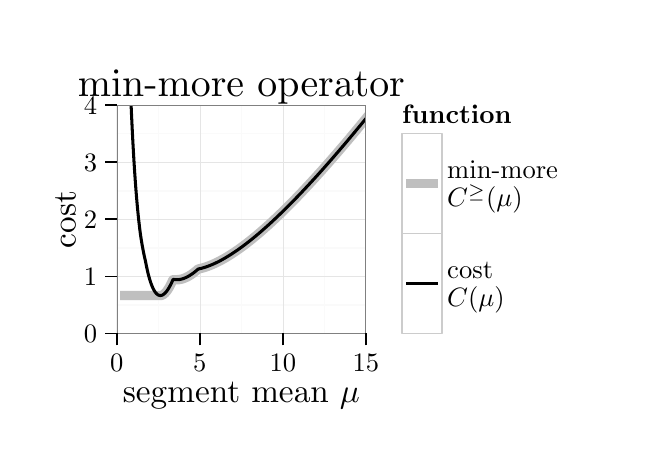
\begin{tikzpicture}[x=1pt,y=1pt]
\definecolor[named]{fillColor}{rgb}{1.00,1.00,1.00}
\path[use as bounding box,fill=fillColor,fill opacity=0.00] (0,0) rectangle (216.81,144.54);
\begin{scope}
\path[clip] (  0.00,  0.00) rectangle (216.81,144.54);
\definecolor[named]{drawColor}{rgb}{1.00,1.00,1.00}
\definecolor[named]{fillColor}{rgb}{1.00,1.00,1.00}

\path[draw=drawColor,line width= 0.6pt,line join=round,line cap=round,fill=fillColor] (  0.00,  0.00) rectangle (216.81,144.54);
\end{scope}
\begin{scope}
\path[clip] ( 32.22, 34.03) rectangle (122.22,116.55);
\definecolor[named]{fillColor}{rgb}{1.00,1.00,1.00}

\path[fill=fillColor] ( 32.22, 34.03) rectangle (122.22,116.55);
\definecolor[named]{drawColor}{rgb}{0.98,0.98,0.98}

\path[draw=drawColor,line width= 0.6pt,line join=round] ( 32.22, 44.35) --
	(122.22, 44.35);

\path[draw=drawColor,line width= 0.6pt,line join=round] ( 32.22, 64.98) --
	(122.22, 64.98);

\path[draw=drawColor,line width= 0.6pt,line join=round] ( 32.22, 85.61) --
	(122.22, 85.61);

\path[draw=drawColor,line width= 0.6pt,line join=round] ( 32.22,106.24) --
	(122.22,106.24);

\path[draw=drawColor,line width= 0.6pt,line join=round] ( 47.22, 34.03) --
	( 47.22,116.55);

\path[draw=drawColor,line width= 0.6pt,line join=round] ( 77.22, 34.03) --
	( 77.22,116.55);

\path[draw=drawColor,line width= 0.6pt,line join=round] (107.22, 34.03) --
	(107.22,116.55);
\definecolor[named]{drawColor}{rgb}{0.90,0.90,0.90}

\path[draw=drawColor,line width= 0.2pt,line join=round] ( 32.22, 34.03) --
	(122.22, 34.03);

\path[draw=drawColor,line width= 0.2pt,line join=round] ( 32.22, 54.66) --
	(122.22, 54.66);

\path[draw=drawColor,line width= 0.2pt,line join=round] ( 32.22, 75.29) --
	(122.22, 75.29);

\path[draw=drawColor,line width= 0.2pt,line join=round] ( 32.22, 95.92) --
	(122.22, 95.92);

\path[draw=drawColor,line width= 0.2pt,line join=round] ( 32.22,116.55) --
	(122.22,116.55);

\path[draw=drawColor,line width= 0.2pt,line join=round] ( 32.22, 34.03) --
	( 32.22,116.55);

\path[draw=drawColor,line width= 0.2pt,line join=round] ( 62.22, 34.03) --
	( 62.22,116.55);

\path[draw=drawColor,line width= 0.2pt,line join=round] ( 92.22, 34.03) --
	( 92.22,116.55);

\path[draw=drawColor,line width= 0.2pt,line join=round] (122.22, 34.03) --
	(122.22,116.55);
\definecolor[named]{drawColor}{rgb}{0.75,0.75,0.75}

\path[draw=drawColor,line width= 3.4pt,line join=round] ( 33.40, 47.76) --
	( 33.55, 47.76) --
	( 33.70, 47.76) --
	( 33.84, 47.76) --
	( 33.99, 47.76) --
	( 34.14, 47.76) --
	( 34.28, 47.76) --
	( 34.43, 47.76) --
	( 34.58, 47.76) --
	( 34.73, 47.76) --
	( 34.87, 47.76) --
	( 35.02, 47.76) --
	( 35.17, 47.76) --
	( 35.31, 47.76) --
	( 35.46, 47.76) --
	( 35.61, 47.76) --
	( 35.75, 47.76) --
	( 35.90, 47.76) --
	( 36.05, 47.76) --
	( 36.19, 47.76) --
	( 36.34, 47.76) --
	( 36.49, 47.76) --
	( 36.63, 47.76) --
	( 36.78, 47.76) --
	( 36.93, 47.76) --
	( 37.08, 47.76) --
	( 37.22, 47.76) --
	( 37.37, 47.76) --
	( 37.52, 47.76) --
	( 37.66, 47.76) --
	( 37.81, 47.76) --
	( 37.96, 47.76) --
	( 38.10, 47.76) --
	( 38.25, 47.76) --
	( 38.40, 47.76) --
	( 38.54, 47.76) --
	( 38.69, 47.76) --
	( 38.84, 47.76) --
	( 38.98, 47.76) --
	( 39.13, 47.76) --
	( 39.28, 47.76) --
	( 39.43, 47.76) --
	( 39.57, 47.76) --
	( 39.72, 47.76) --
	( 39.87, 47.76) --
	( 40.01, 47.76) --
	( 40.16, 47.76) --
	( 40.31, 47.76) --
	( 40.45, 47.76) --
	( 40.60, 47.76) --
	( 40.75, 47.76) --
	( 40.89, 47.76) --
	( 41.04, 47.76) --
	( 41.19, 47.76) --
	( 41.34, 47.76) --
	( 41.48, 47.76) --
	( 41.63, 47.76) --
	( 41.78, 47.76) --
	( 41.92, 47.76) --
	( 42.07, 47.76) --
	( 42.22, 47.76) --
	( 42.36, 47.76) --
	( 42.51, 47.76) --
	( 42.66, 47.76) --
	( 42.80, 47.76) --
	( 42.95, 47.76) --
	( 43.10, 47.76) --
	( 43.24, 47.76) --
	( 43.39, 47.76) --
	( 43.54, 47.76) --
	( 43.69, 47.76) --
	( 43.83, 47.76) --
	( 43.98, 47.76) --
	( 44.13, 47.76) --
	( 44.27, 47.76) --
	( 44.42, 47.76) --
	( 44.57, 47.76) --
	( 44.71, 47.76) --
	( 44.86, 47.76) --
	( 45.01, 47.76) --
	( 45.15, 47.76) --
	( 45.30, 47.76) --
	( 45.45, 47.76) --
	( 45.59, 47.76) --
	( 45.74, 47.76) --
	( 45.89, 47.76) --
	( 46.04, 47.76) --
	( 46.18, 47.76) --
	( 46.33, 47.76) --
	( 46.48, 47.76) --
	( 46.62, 47.76) --
	( 46.77, 47.76) --
	( 46.92, 47.76) --
	( 47.06, 47.76) --
	( 47.21, 47.76) --
	( 47.36, 47.76) --
	( 47.50, 47.76) --
	( 47.65, 47.76) --
	( 47.80, 47.76) --
	( 47.94, 47.76) --
	( 47.94, 47.76) --
	( 47.99, 47.76) --
	( 48.04, 47.76) --
	( 48.08, 47.76) --
	( 48.13, 47.77) --
	( 48.17, 47.77) --
	( 48.22, 47.78) --
	( 48.27, 47.79) --
	( 48.31, 47.80) --
	( 48.36, 47.81) --
	( 48.40, 47.82) --
	( 48.45, 47.84) --
	( 48.50, 47.85) --
	( 48.54, 47.87) --
	( 48.59, 47.89) --
	( 48.63, 47.91) --
	( 48.68, 47.93) --
	( 48.73, 47.95) --
	( 48.77, 47.97) --
	( 48.82, 48.00) --
	( 48.86, 48.02) --
	( 48.91, 48.05) --
	( 48.95, 48.08) --
	( 49.00, 48.11) --
	( 49.05, 48.14) --
	( 49.09, 48.17) --
	( 49.14, 48.20) --
	( 49.18, 48.24) --
	( 49.23, 48.27) --
	( 49.28, 48.31) --
	( 49.32, 48.35) --
	( 49.37, 48.38) --
	( 49.41, 48.42) --
	( 49.46, 48.47) --
	( 49.51, 48.51) --
	( 49.55, 48.55) --
	( 49.60, 48.60) --
	( 49.64, 48.64) --
	( 49.69, 48.69) --
	( 49.74, 48.74) --
	( 49.78, 48.78) --
	( 49.83, 48.83) --
	( 49.87, 48.89) --
	( 49.92, 48.94) --
	( 49.97, 48.99) --
	( 50.01, 49.05) --
	( 50.06, 49.10) --
	( 50.10, 49.16) --
	( 50.15, 49.22) --
	( 50.19, 49.27) --
	( 50.24, 49.33) --
	( 50.29, 49.40) --
	( 50.33, 49.46) --
	( 50.38, 49.52) --
	( 50.42, 49.58) --
	( 50.47, 49.65) --
	( 50.52, 49.72) --
	( 50.56, 49.78) --
	( 50.61, 49.85) --
	( 50.65, 49.92) --
	( 50.70, 49.99) --
	( 50.75, 50.06) --
	( 50.79, 50.13) --
	( 50.84, 50.21) --
	( 50.88, 50.28) --
	( 50.93, 50.36) --
	( 50.98, 50.43) --
	( 51.02, 50.51) --
	( 51.07, 50.59) --
	( 51.11, 50.67) --
	( 51.16, 50.75) --
	( 51.21, 50.83) --
	( 51.25, 50.91) --
	( 51.30, 50.99) --
	( 51.34, 51.07) --
	( 51.39, 51.16) --
	( 51.43, 51.25) --
	( 51.48, 51.33) --
	( 51.53, 51.42) --
	( 51.57, 51.51) --
	( 51.62, 51.60) --
	( 51.66, 51.69) --
	( 51.71, 51.78) --
	( 51.76, 51.87) --
	( 51.80, 51.96) --
	( 51.85, 52.06) --
	( 51.89, 52.15) --
	( 51.94, 52.25) --
	( 51.99, 52.34) --
	( 52.03, 52.44) --
	( 52.08, 52.54) --
	( 52.12, 52.64) --
	( 52.17, 52.74) --
	( 52.22, 52.84) --
	( 52.26, 52.94) --
	( 52.31, 53.04) --
	( 52.35, 53.15) --
	( 52.40, 53.25) --
	( 52.45, 53.35) --
	( 52.49, 53.46) --
	( 52.49, 53.46) --
	( 52.50, 53.46) --
	( 52.52, 53.46) --
	( 52.53, 53.46) --
	( 52.55, 53.46) --
	( 52.56, 53.46) --
	( 52.57, 53.46) --
	( 52.59, 53.46) --
	( 52.60, 53.46) --
	( 52.62, 53.46) --
	( 52.63, 53.46) --
	( 52.64, 53.46) --
	( 52.66, 53.46) --
	( 52.67, 53.46) --
	( 52.68, 53.46) --
	( 52.70, 53.46) --
	( 52.71, 53.46) --
	( 52.73, 53.46) --
	( 52.74, 53.46) --
	( 52.75, 53.46) --
	( 52.77, 53.46) --
	( 52.78, 53.46) --
	( 52.80, 53.46) --
	( 52.81, 53.46) --
	( 52.82, 53.46) --
	( 52.84, 53.46) --
	( 52.85, 53.46) --
	( 52.86, 53.46) --
	( 52.88, 53.46) --
	( 52.89, 53.46) --
	( 52.91, 53.46) --
	( 52.92, 53.46) --
	( 52.93, 53.46) --
	( 52.95, 53.46) --
	( 52.96, 53.46) --
	( 52.97, 53.46) --
	( 52.99, 53.46) --
	( 53.00, 53.46) --
	( 53.02, 53.46) --
	( 53.03, 53.46) --
	( 53.04, 53.46) --
	( 53.06, 53.46) --
	( 53.07, 53.46) --
	( 53.09, 53.46) --
	( 53.10, 53.46) --
	( 53.11, 53.46) --
	( 53.13, 53.46) --
	( 53.14, 53.46) --
	( 53.15, 53.46) --
	( 53.17, 53.46) --
	( 53.18, 53.46) --
	( 53.20, 53.46) --
	( 53.21, 53.46) --
	( 53.22, 53.46) --
	( 53.24, 53.46) --
	( 53.25, 53.46) --
	( 53.26, 53.46) --
	( 53.28, 53.46) --
	( 53.29, 53.46) --
	( 53.31, 53.46) --
	( 53.32, 53.46) --
	( 53.33, 53.46) --
	( 53.35, 53.46) --
	( 53.36, 53.46) --
	( 53.38, 53.46) --
	( 53.39, 53.46) --
	( 53.40, 53.46) --
	( 53.42, 53.46) --
	( 53.43, 53.46) --
	( 53.44, 53.46) --
	( 53.46, 53.46) --
	( 53.47, 53.46) --
	( 53.49, 53.46) --
	( 53.50, 53.46) --
	( 53.51, 53.46) --
	( 53.53, 53.46) --
	( 53.54, 53.46) --
	( 53.56, 53.46) --
	( 53.57, 53.46) --
	( 53.58, 53.46) --
	( 53.60, 53.46) --
	( 53.61, 53.46) --
	( 53.62, 53.46) --
	( 53.64, 53.46) --
	( 53.65, 53.46) --
	( 53.67, 53.46) --
	( 53.68, 53.46) --
	( 53.69, 53.46) --
	( 53.71, 53.46) --
	( 53.72, 53.46) --
	( 53.73, 53.46) --
	( 53.75, 53.46) --
	( 53.76, 53.46) --
	( 53.78, 53.46) --
	( 53.79, 53.46) --
	( 53.80, 53.46) --
	( 53.82, 53.46) --
	( 53.83, 53.46) --
	( 53.85, 53.46) --
	( 53.86, 53.46) --
	( 53.86, 53.46) --
	( 53.94, 53.46) --
	( 54.02, 53.46) --
	( 54.09, 53.47) --
	( 54.17, 53.47) --
	( 54.25, 53.47) --
	( 54.33, 53.48) --
	( 54.41, 53.48) --
	( 54.48, 53.49) --
	( 54.56, 53.50) --
	( 54.64, 53.51) --
	( 54.72, 53.52) --
	( 54.80, 53.53) --
	( 54.87, 53.54) --
	( 54.95, 53.55) --
	( 55.03, 53.57) --
	( 55.11, 53.58) --
	( 55.19, 53.60) --
	( 55.26, 53.61) --
	( 55.34, 53.63) --
	( 55.42, 53.65) --
	( 55.50, 53.66) --
	( 55.58, 53.68) --
	( 55.65, 53.70) --
	( 55.73, 53.72) --
	( 55.81, 53.75) --
	( 55.89, 53.77) --
	( 55.97, 53.79) --
	( 56.04, 53.82) --
	( 56.12, 53.84) --
	( 56.20, 53.87) --
	( 56.28, 53.89) --
	( 56.36, 53.92) --
	( 56.43, 53.95) --
	( 56.51, 53.98) --
	( 56.59, 54.01) --
	( 56.67, 54.04) --
	( 56.75, 54.07) --
	( 56.82, 54.10) --
	( 56.90, 54.13) --
	( 56.98, 54.17) --
	( 57.06, 54.20) --
	( 57.14, 54.24) --
	( 57.21, 54.27) --
	( 57.29, 54.31) --
	( 57.37, 54.35) --
	( 57.45, 54.38) --
	( 57.53, 54.42) --
	( 57.60, 54.46) --
	( 57.68, 54.50) --
	( 57.76, 54.54) --
	( 57.84, 54.58) --
	( 57.92, 54.62) --
	( 57.99, 54.67) --
	( 58.07, 54.71) --
	( 58.15, 54.75) --
	( 58.23, 54.80) --
	( 58.31, 54.84) --
	( 58.38, 54.89) --
	( 58.46, 54.94) --
	( 58.54, 54.98) --
	( 58.62, 55.03) --
	( 58.70, 55.08) --
	( 58.77, 55.13) --
	( 58.85, 55.18) --
	( 58.93, 55.23) --
	( 59.01, 55.28) --
	( 59.09, 55.33) --
	( 59.16, 55.39) --
	( 59.24, 55.44) --
	( 59.32, 55.49) --
	( 59.40, 55.55) --
	( 59.48, 55.60) --
	( 59.55, 55.66) --
	( 59.63, 55.72) --
	( 59.71, 55.77) --
	( 59.79, 55.83) --
	( 59.87, 55.89) --
	( 59.94, 55.95) --
	( 60.02, 56.00) --
	( 60.10, 56.06) --
	( 60.18, 56.13) --
	( 60.26, 56.19) --
	( 60.33, 56.25) --
	( 60.41, 56.31) --
	( 60.49, 56.37) --
	( 60.57, 56.44) --
	( 60.65, 56.50) --
	( 60.72, 56.56) --
	( 60.80, 56.63) --
	( 60.88, 56.69) --
	( 60.96, 56.76) --
	( 61.04, 56.83) --
	( 61.11, 56.89) --
	( 61.19, 56.96) --
	( 61.27, 57.03) --
	( 61.35, 57.10) --
	( 61.43, 57.17) --
	( 61.50, 57.24) --
	( 61.58, 57.31) --
	( 61.58, 57.31) --
	( 62.58, 57.54) --
	( 63.58, 57.81) --
	( 64.59, 58.14) --
	( 65.59, 58.50) --
	( 66.59, 58.91) --
	( 67.59, 59.35) --
	( 68.59, 59.83) --
	( 69.60, 60.34) --
	( 70.60, 60.89) --
	( 71.60, 61.46) --
	( 72.60, 62.07) --
	( 73.60, 62.70) --
	( 74.60, 63.36) --
	( 75.61, 64.04) --
	( 76.61, 64.75) --
	( 77.61, 65.47) --
	( 78.61, 66.23) --
	( 79.61, 67.00) --
	( 80.62, 67.79) --
	( 81.62, 68.60) --
	( 82.62, 69.43) --
	( 83.62, 70.27) --
	( 84.62, 71.14) --
	( 85.62, 72.02) --
	( 86.63, 72.91) --
	( 87.63, 73.82) --
	( 88.63, 74.75) --
	( 89.63, 75.69) --
	( 90.63, 76.64) --
	( 91.63, 77.60) --
	( 92.64, 78.58) --
	( 93.64, 79.57) --
	( 94.64, 80.57) --
	( 95.64, 81.59) --
	( 96.64, 82.61) --
	( 97.65, 83.65) --
	( 98.65, 84.69) --
	( 99.65, 85.75) --
	(100.65, 86.82) --
	(101.65, 87.89) --
	(102.65, 88.98) --
	(103.66, 90.07) --
	(104.66, 91.17) --
	(105.66, 92.28) --
	(106.66, 93.40) --
	(107.66, 94.53) --
	(108.66, 95.66) --
	(109.67, 96.81) --
	(110.67, 97.96) --
	(111.67, 99.12) --
	(112.67,100.28) --
	(113.67,101.45) --
	(114.68,102.63) --
	(115.68,103.81) --
	(116.68,105.01) --
	(117.68,106.20) --
	(118.68,107.41) --
	(119.68,108.62) --
	(120.69,109.83) --
	(121.69,111.05) --
	(122.69,112.28) --
	(123.69,113.51) --
	(124.69,114.75) --
	(125.69,115.99) --
	(126.70,117.24) --
	(127.70,118.49) --
	(128.70,119.75) --
	(129.70,121.01) --
	(130.70,122.28) --
	(131.71,123.55) --
	(132.71,124.83) --
	(133.71,126.11) --
	(134.71,127.39) --
	(135.71,128.68) --
	(136.71,129.98) --
	(137.72,131.28) --
	(138.72,132.58) --
	(139.72,133.88) --
	(140.72,135.19) --
	(141.72,136.51) --
	(142.73,137.82) --
	(143.73,139.14) --
	(144.73,140.47) --
	(145.73,141.80) --
	(146.73,143.13) --
	(147.73,144.46) --
	(147.79,144.54);
\definecolor[named]{drawColor}{rgb}{0.00,0.00,0.00}

\path[draw=drawColor,line width= 1.1pt,line join=round] ( 36.37,144.54) --
	( 36.37,144.21) --
	( 36.45,141.63) --
	( 36.53,139.12) --
	( 36.61,136.68) --
	( 36.69,134.31) --
	( 36.77,132.01) --
	( 36.85,129.77) --
	( 36.93,127.59) --
	( 37.01,125.48) --
	( 37.09,123.42) --
	( 37.17,121.41) --
	( 37.25,119.46) --
	( 37.33,117.56) --
	( 37.41,115.72) --
	( 37.49,113.92) --
	( 37.57,112.17) --
	( 37.65,110.46) --
	( 37.73,108.80) --
	( 37.81,107.19) --
	( 37.89,105.61) --
	( 37.97,104.08) --
	( 38.05,102.59) --
	( 38.13,101.14) --
	( 38.21, 99.72) --
	( 38.29, 98.34) --
	( 38.37, 97.00) --
	( 38.45, 95.69) --
	( 38.53, 94.42) --
	( 38.61, 93.18) --
	( 38.69, 91.97) --
	( 38.77, 90.79) --
	( 38.85, 89.65) --
	( 38.93, 88.53) --
	( 39.01, 87.45) --
	( 39.09, 86.39) --
	( 39.17, 85.36) --
	( 39.25, 84.36) --
	( 39.33, 83.39) --
	( 39.41, 82.44) --
	( 39.49, 81.52) --
	( 39.57, 80.62) --
	( 39.65, 79.74) --
	( 39.73, 78.90) --
	( 39.81, 78.07) --
	( 39.89, 77.27) --
	( 39.97, 76.49) --
	( 40.05, 75.73) --
	( 40.13, 74.99) --
	( 40.21, 74.28) --
	( 40.29, 73.58) --
	( 40.37, 72.91) --
	( 40.44, 72.25) --
	( 40.52, 71.62) --
	( 40.60, 71.00) --
	( 40.68, 70.41) --
	( 40.76, 69.83) --
	( 40.84, 69.27) --
	( 40.92, 68.73) --
	( 41.00, 68.20) --
	( 41.08, 67.69) --
	( 41.16, 67.20) --
	( 41.24, 66.73) --
	( 41.32, 66.27) --
	( 41.40, 65.83) --
	( 41.48, 65.40) --
	( 41.56, 64.99) --
	( 41.56, 64.99) --
	( 41.57, 64.93) --
	( 41.58, 64.88) --
	( 41.59, 64.82) --
	( 41.60, 64.76) --
	( 41.61, 64.71) --
	( 41.62, 64.65) --
	( 41.63, 64.59) --
	( 41.64, 64.54) --
	( 41.65, 64.48) --
	( 41.66, 64.43) --
	( 41.67, 64.37) --
	( 41.68, 64.32) --
	( 41.69, 64.26) --
	( 41.70, 64.21) --
	( 41.71, 64.15) --
	( 41.72, 64.10) --
	( 41.73, 64.04) --
	( 41.74, 63.99) --
	( 41.75, 63.94) --
	( 41.76, 63.88) --
	( 41.77, 63.83) --
	( 41.78, 63.78) --
	( 41.79, 63.72) --
	( 41.80, 63.67) --
	( 41.81, 63.62) --
	( 41.82, 63.57) --
	( 41.83, 63.52) --
	( 41.84, 63.46) --
	( 41.85, 63.41) --
	( 41.86, 63.36) --
	( 41.87, 63.31) --
	( 41.88, 63.26) --
	( 41.89, 63.21) --
	( 41.90, 63.16) --
	( 41.91, 63.11) --
	( 41.92, 63.06) --
	( 41.93, 63.01) --
	( 41.94, 62.96) --
	( 41.95, 62.91) --
	( 41.96, 62.86) --
	( 41.97, 62.81) --
	( 41.98, 62.76) --
	( 41.99, 62.71) --
	( 42.00, 62.67) --
	( 42.01, 62.62) --
	( 42.02, 62.57) --
	( 42.03, 62.52) --
	( 42.04, 62.48) --
	( 42.05, 62.43) --
	( 42.06, 62.38) --
	( 42.07, 62.33) --
	( 42.08, 62.29) --
	( 42.09, 62.24) --
	( 42.10, 62.19) --
	( 42.11, 62.15) --
	( 42.12, 62.10) --
	( 42.13, 62.06) --
	( 42.14, 62.01) --
	( 42.15, 61.97) --
	( 42.16, 61.92) --
	( 42.17, 61.88) --
	( 42.18, 61.83) --
	( 42.19, 61.79) --
	( 42.20, 61.74) --
	( 42.21, 61.70) --
	( 42.22, 61.65) --
	( 42.22, 61.61) --
	( 42.23, 61.57) --
	( 42.24, 61.52) --
	( 42.25, 61.48) --
	( 42.26, 61.44) --
	( 42.27, 61.39) --
	( 42.28, 61.35) --
	( 42.29, 61.31) --
	( 42.30, 61.27) --
	( 42.31, 61.23) --
	( 42.32, 61.18) --
	( 42.33, 61.14) --
	( 42.34, 61.10) --
	( 42.35, 61.06) --
	( 42.36, 61.02) --
	( 42.37, 60.98) --
	( 42.38, 60.94) --
	( 42.39, 60.90) --
	( 42.40, 60.86) --
	( 42.41, 60.82) --
	( 42.42, 60.78) --
	( 42.43, 60.74) --
	( 42.44, 60.70) --
	( 42.45, 60.66) --
	( 42.46, 60.62) --
	( 42.47, 60.58) --
	( 42.48, 60.54) --
	( 42.49, 60.50) --
	( 42.50, 60.46) --
	( 42.51, 60.43) --
	( 42.52, 60.39) --
	( 42.53, 60.35) --
	( 42.54, 60.31) --
	( 42.54, 60.31) --
	( 42.64, 59.77) --
	( 42.74, 59.25) --
	( 42.84, 58.74) --
	( 42.95, 58.25) --
	( 43.05, 57.77) --
	( 43.15, 57.31) --
	( 43.25, 56.85) --
	( 43.35, 56.42) --
	( 43.45, 55.99) --
	( 43.55, 55.58) --
	( 43.65, 55.18) --
	( 43.75, 54.80) --
	( 43.86, 54.43) --
	( 43.96, 54.07) --
	( 44.06, 53.72) --
	( 44.16, 53.38) --
	( 44.26, 53.06) --
	( 44.36, 52.74) --
	( 44.46, 52.44) --
	( 44.56, 52.15) --
	( 44.66, 51.87) --
	( 44.77, 51.60) --
	( 44.87, 51.34) --
	( 44.97, 51.09) --
	( 45.07, 50.85) --
	( 45.17, 50.62) --
	( 45.27, 50.41) --
	( 45.37, 50.20) --
	( 45.47, 50.00) --
	( 45.57, 49.81) --
	( 45.68, 49.63) --
	( 45.78, 49.46) --
	( 45.88, 49.29) --
	( 45.98, 49.14) --
	( 46.08, 49.00) --
	( 46.18, 48.86) --
	( 46.28, 48.73) --
	( 46.38, 48.61) --
	( 46.48, 48.50) --
	( 46.59, 48.40) --
	( 46.69, 48.30) --
	( 46.79, 48.22) --
	( 46.89, 48.14) --
	( 46.99, 48.07) --
	( 47.09, 48.00) --
	( 47.19, 47.95) --
	( 47.29, 47.90) --
	( 47.40, 47.86) --
	( 47.50, 47.82) --
	( 47.60, 47.80) --
	( 47.70, 47.78) --
	( 47.80, 47.76) --
	( 47.90, 47.76) --
	( 48.00, 47.76) --
	( 48.10, 47.77) --
	( 48.20, 47.78) --
	( 48.31, 47.80) --
	( 48.41, 47.83) --
	( 48.51, 47.86) --
	( 48.61, 47.90) --
	( 48.71, 47.94) --
	( 48.81, 47.99) --
	( 48.91, 48.05) --
	( 49.01, 48.12) --
	( 49.11, 48.18) --
	( 49.22, 48.26) --
	( 49.32, 48.34) --
	( 49.42, 48.43) --
	( 49.52, 48.52) --
	( 49.62, 48.62) --
	( 49.72, 48.72) --
	( 49.82, 48.83) --
	( 49.92, 48.94) --
	( 50.02, 49.06) --
	( 50.13, 49.19) --
	( 50.23, 49.32) --
	( 50.33, 49.45) --
	( 50.43, 49.59) --
	( 50.53, 49.73) --
	( 50.63, 49.88) --
	( 50.73, 50.04) --
	( 50.83, 50.20) --
	( 50.93, 50.36) --
	( 51.04, 50.53) --
	( 51.14, 50.71) --
	( 51.24, 50.88) --
	( 51.34, 51.07) --
	( 51.44, 51.25) --
	( 51.54, 51.45) --
	( 51.64, 51.64) --
	( 51.74, 51.84) --
	( 51.84, 52.05) --
	( 51.95, 52.26) --
	( 52.05, 52.47) --
	( 52.15, 52.69) --
	( 52.25, 52.91) --
	( 52.35, 53.14) --
	( 52.45, 53.37) --
	( 52.55, 53.60) --
	( 52.55, 53.60) --
	( 52.64, 53.58) --
	( 52.73, 53.57) --
	( 52.83, 53.55) --
	( 52.92, 53.53) --
	( 53.01, 53.52) --
	( 53.10, 53.51) --
	( 53.19, 53.50) --
	( 53.28, 53.49) --
	( 53.37, 53.48) --
	( 53.46, 53.47) --
	( 53.56, 53.47) --
	( 53.65, 53.46) --
	( 53.74, 53.46) --
	( 53.83, 53.46) --
	( 53.92, 53.46) --
	( 54.01, 53.46) --
	( 54.10, 53.47) --
	( 54.19, 53.47) --
	( 54.28, 53.48) --
	( 54.38, 53.48) --
	( 54.47, 53.49) --
	( 54.56, 53.50) --
	( 54.65, 53.51) --
	( 54.74, 53.52) --
	( 54.83, 53.53) --
	( 54.92, 53.55) --
	( 55.01, 53.56) --
	( 55.11, 53.58) --
	( 55.20, 53.60) --
	( 55.29, 53.62) --
	( 55.38, 53.64) --
	( 55.47, 53.66) --
	( 55.56, 53.68) --
	( 55.65, 53.70) --
	( 55.74, 53.73) --
	( 55.84, 53.75) --
	( 55.93, 53.78) --
	( 56.02, 53.81) --
	( 56.11, 53.84) --
	( 56.20, 53.87) --
	( 56.29, 53.90) --
	( 56.38, 53.93) --
	( 56.47, 53.96) --
	( 56.56, 54.00) --
	( 56.66, 54.03) --
	( 56.75, 54.07) --
	( 56.84, 54.11) --
	( 56.93, 54.15) --
	( 57.02, 54.19) --
	( 57.11, 54.23) --
	( 57.20, 54.27) --
	( 57.29, 54.31) --
	( 57.39, 54.35) --
	( 57.48, 54.40) --
	( 57.57, 54.44) --
	( 57.66, 54.49) --
	( 57.75, 54.54) --
	( 57.84, 54.59) --
	( 57.93, 54.63) --
	( 58.02, 54.68) --
	( 58.12, 54.74) --
	( 58.21, 54.79) --
	( 58.30, 54.84) --
	( 58.39, 54.89) --
	( 58.48, 54.95) --
	( 58.57, 55.00) --
	( 58.66, 55.06) --
	( 58.75, 55.12) --
	( 58.85, 55.18) --
	( 58.94, 55.24) --
	( 59.03, 55.30) --
	( 59.12, 55.36) --
	( 59.21, 55.42) --
	( 59.30, 55.48) --
	( 59.39, 55.54) --
	( 59.48, 55.61) --
	( 59.57, 55.67) --
	( 59.67, 55.74) --
	( 59.76, 55.81) --
	( 59.85, 55.87) --
	( 59.94, 55.94) --
	( 60.03, 56.01) --
	( 60.12, 56.08) --
	( 60.21, 56.15) --
	( 60.30, 56.22) --
	( 60.40, 56.30) --
	( 60.49, 56.37) --
	( 60.58, 56.44) --
	( 60.67, 56.52) --
	( 60.76, 56.59) --
	( 60.85, 56.67) --
	( 60.94, 56.75) --
	( 61.03, 56.83) --
	( 61.13, 56.90) --
	( 61.22, 56.98) --
	( 61.31, 57.06) --
	( 61.40, 57.14) --
	( 61.49, 57.22) --
	( 61.58, 57.31) --
	( 61.58, 57.31) --
	( 62.58, 57.54) --
	( 63.58, 57.81) --
	( 64.59, 58.14) --
	( 65.59, 58.50) --
	( 66.59, 58.91) --
	( 67.59, 59.35) --
	( 68.59, 59.83) --
	( 69.60, 60.34) --
	( 70.60, 60.89) --
	( 71.60, 61.46) --
	( 72.60, 62.07) --
	( 73.60, 62.70) --
	( 74.60, 63.36) --
	( 75.61, 64.04) --
	( 76.61, 64.75) --
	( 77.61, 65.47) --
	( 78.61, 66.23) --
	( 79.61, 67.00) --
	( 80.62, 67.79) --
	( 81.62, 68.60) --
	( 82.62, 69.43) --
	( 83.62, 70.27) --
	( 84.62, 71.14) --
	( 85.62, 72.02) --
	( 86.63, 72.91) --
	( 87.63, 73.82) --
	( 88.63, 74.75) --
	( 89.63, 75.69) --
	( 90.63, 76.64) --
	( 91.63, 77.60) --
	( 92.64, 78.58) --
	( 93.64, 79.57) --
	( 94.64, 80.57) --
	( 95.64, 81.59) --
	( 96.64, 82.61) --
	( 97.65, 83.65) --
	( 98.65, 84.69) --
	( 99.65, 85.75) --
	(100.65, 86.82) --
	(101.65, 87.89) --
	(102.65, 88.98) --
	(103.66, 90.07) --
	(104.66, 91.17) --
	(105.66, 92.28) --
	(106.66, 93.40) --
	(107.66, 94.53) --
	(108.66, 95.66) --
	(109.67, 96.81) --
	(110.67, 97.96) --
	(111.67, 99.12) --
	(112.67,100.28) --
	(113.67,101.45) --
	(114.68,102.63) --
	(115.68,103.81) --
	(116.68,105.01) --
	(117.68,106.20) --
	(118.68,107.41) --
	(119.68,108.62) --
	(120.69,109.83) --
	(121.69,111.05) --
	(122.69,112.28) --
	(123.69,113.51) --
	(124.69,114.75) --
	(125.69,115.99) --
	(126.70,117.24) --
	(127.70,118.49) --
	(128.70,119.75) --
	(129.70,121.01) --
	(130.70,122.28) --
	(131.71,123.55) --
	(132.71,124.83) --
	(133.71,126.11) --
	(134.71,127.39) --
	(135.71,128.68) --
	(136.71,129.98) --
	(137.72,131.28) --
	(138.72,132.58) --
	(139.72,133.88) --
	(140.72,135.19) --
	(141.72,136.51) --
	(142.73,137.82) --
	(143.73,139.14) --
	(144.73,140.47) --
	(145.73,141.80) --
	(146.73,143.13) --
	(147.73,144.46) --
	(147.79,144.54);
\definecolor[named]{drawColor}{rgb}{0.50,0.50,0.50}

\path[draw=drawColor,line width= 0.6pt,line join=round,line cap=round] ( 32.22, 34.03) rectangle (122.22,116.55);
\end{scope}
\begin{scope}
\path[clip] (  0.00,  0.00) rectangle (216.81,144.54);
\definecolor[named]{drawColor}{rgb}{0.00,0.00,0.00}

\node[text=drawColor,anchor=base east,inner sep=0pt, outer sep=0pt, scale=  0.96] at ( 25.11, 30.73) {0};

\node[text=drawColor,anchor=base east,inner sep=0pt, outer sep=0pt, scale=  0.96] at ( 25.11, 51.36) {1};

\node[text=drawColor,anchor=base east,inner sep=0pt, outer sep=0pt, scale=  0.96] at ( 25.11, 71.99) {2};

\node[text=drawColor,anchor=base east,inner sep=0pt, outer sep=0pt, scale=  0.96] at ( 25.11, 92.62) {3};

\node[text=drawColor,anchor=base east,inner sep=0pt, outer sep=0pt, scale=  0.96] at ( 25.11,113.25) {4};
\end{scope}
\begin{scope}
\path[clip] (  0.00,  0.00) rectangle (216.81,144.54);
\definecolor[named]{drawColor}{rgb}{0.00,0.00,0.00}

\path[draw=drawColor,line width= 0.6pt,line join=round] ( 27.95, 34.03) --
	( 32.22, 34.03);

\path[draw=drawColor,line width= 0.6pt,line join=round] ( 27.95, 54.66) --
	( 32.22, 54.66);

\path[draw=drawColor,line width= 0.6pt,line join=round] ( 27.95, 75.29) --
	( 32.22, 75.29);

\path[draw=drawColor,line width= 0.6pt,line join=round] ( 27.95, 95.92) --
	( 32.22, 95.92);

\path[draw=drawColor,line width= 0.6pt,line join=round] ( 27.95,116.55) --
	( 32.22,116.55);
\end{scope}
\begin{scope}
\path[clip] (  0.00,  0.00) rectangle (216.81,144.54);
\definecolor[named]{drawColor}{rgb}{0.00,0.00,0.00}

\path[draw=drawColor,line width= 0.6pt,line join=round] ( 32.22, 29.77) --
	( 32.22, 34.03);

\path[draw=drawColor,line width= 0.6pt,line join=round] ( 62.22, 29.77) --
	( 62.22, 34.03);

\path[draw=drawColor,line width= 0.6pt,line join=round] ( 92.22, 29.77) --
	( 92.22, 34.03);

\path[draw=drawColor,line width= 0.6pt,line join=round] (122.22, 29.77) --
	(122.22, 34.03);
\end{scope}
\begin{scope}
\path[clip] (  0.00,  0.00) rectangle (216.81,144.54);
\definecolor[named]{drawColor}{rgb}{0.00,0.00,0.00}

\node[text=drawColor,anchor=base,inner sep=0pt, outer sep=0pt, scale=  0.96] at ( 32.22, 20.31) {0};

\node[text=drawColor,anchor=base,inner sep=0pt, outer sep=0pt, scale=  0.96] at ( 62.22, 20.31) {5};

\node[text=drawColor,anchor=base,inner sep=0pt, outer sep=0pt, scale=  0.96] at ( 92.22, 20.31) {10};

\node[text=drawColor,anchor=base,inner sep=0pt, outer sep=0pt, scale=  0.96] at (122.22, 20.31) {15};
\end{scope}
\begin{scope}
\path[clip] (  0.00,  0.00) rectangle (216.81,144.54);
\definecolor[named]{drawColor}{rgb}{0.00,0.00,0.00}

\node[text=drawColor,anchor=base,inner sep=0pt, outer sep=0pt, scale=  1.20] at ( 77.22,  9.03) {segment mean $\mu$};
\end{scope}
\begin{scope}
\path[clip] (  0.00,  0.00) rectangle (216.81,144.54);
\definecolor[named]{drawColor}{rgb}{0.00,0.00,0.00}

\node[text=drawColor,rotate= 90.00,anchor=base,inner sep=0pt, outer sep=0pt, scale=  1.20] at ( 17.30, 75.29) {cost};
\end{scope}
\begin{scope}
\path[clip] (  0.00,  0.00) rectangle (216.81,144.54);
\definecolor[named]{fillColor}{rgb}{1.00,1.00,1.00}

\path[fill=fillColor] (131.08, 29.77) rectangle (195.90,120.82);
\end{scope}
\begin{scope}
\path[clip] (  0.00,  0.00) rectangle (216.81,144.54);
\definecolor[named]{drawColor}{rgb}{0.00,0.00,0.00}

\node[text=drawColor,anchor=base west,inner sep=0pt, outer sep=0pt, scale=  0.96] at (135.35,109.92) {\bfseries function};
\end{scope}
\begin{scope}
\path[clip] (  0.00,  0.00) rectangle (216.81,144.54);
\definecolor[named]{drawColor}{rgb}{0.80,0.80,0.80}
\definecolor[named]{fillColor}{rgb}{1.00,1.00,1.00}

\path[draw=drawColor,line width= 0.6pt,line join=round,line cap=round,fill=fillColor] (135.35, 70.18) rectangle (149.81,106.31);
\end{scope}
\begin{scope}
\path[clip] (  0.00,  0.00) rectangle (216.81,144.54);
\definecolor[named]{drawColor}{rgb}{0.75,0.75,0.75}

\path[draw=drawColor,line width= 3.4pt,line join=round] (136.80, 88.24) -- (148.36, 88.24);
\end{scope}
\begin{scope}
\path[clip] (  0.00,  0.00) rectangle (216.81,144.54);
\definecolor[named]{drawColor}{rgb}{0.80,0.80,0.80}
\definecolor[named]{fillColor}{rgb}{1.00,1.00,1.00}

\path[draw=drawColor,line width= 0.6pt,line join=round,line cap=round,fill=fillColor] (135.35, 34.04) rectangle (149.81, 70.18);
\end{scope}
\begin{scope}
\path[clip] (  0.00,  0.00) rectangle (216.81,144.54);
\definecolor[named]{drawColor}{rgb}{0.00,0.00,0.00}

\path[draw=drawColor,line width= 1.1pt,line join=round] (136.80, 52.11) -- (148.36, 52.11);
\end{scope}
\begin{scope}
\path[clip] (  0.00,  0.00) rectangle (216.81,144.54);
\definecolor[named]{drawColor}{rgb}{0.00,0.00,0.00}

\node[text=drawColor,anchor=base west,inner sep=0pt, outer sep=0pt, scale=  0.96] at (151.61, 90.12) {min-more};

\node[text=drawColor,anchor=base west,inner sep=0pt, outer sep=0pt, scale=  0.96] at (151.61, 79.75) {$C^{\geq}(\mu)$};
\end{scope}
\begin{scope}
\path[clip] (  0.00,  0.00) rectangle (216.81,144.54);
\definecolor[named]{drawColor}{rgb}{0.00,0.00,0.00}

\node[text=drawColor,anchor=base west,inner sep=0pt, outer sep=0pt, scale=  0.96] at (151.61, 53.99) {cost};

\node[text=drawColor,anchor=base west,inner sep=0pt, outer sep=0pt, scale=  0.96] at (151.61, 43.62) {$C(\mu)$};
\end{scope}
\begin{scope}
\path[clip] (  0.00,  0.00) rectangle (216.81,144.54);
\definecolor[named]{drawColor}{rgb}{0.00,0.00,0.00}

\node[text=drawColor,anchor=base,inner sep=0pt, outer sep=0pt, scale=  1.44] at ( 77.22,119.57) {min-more operator};
\end{scope}
\end{tikzpicture}

    \end{center}
  }
  \parbox{3in}{
    \begin{center}
      % Created by tikzDevice version 0.9 on 2016-05-12 20:28:50
% !TEX encoding = UTF-8 Unicode
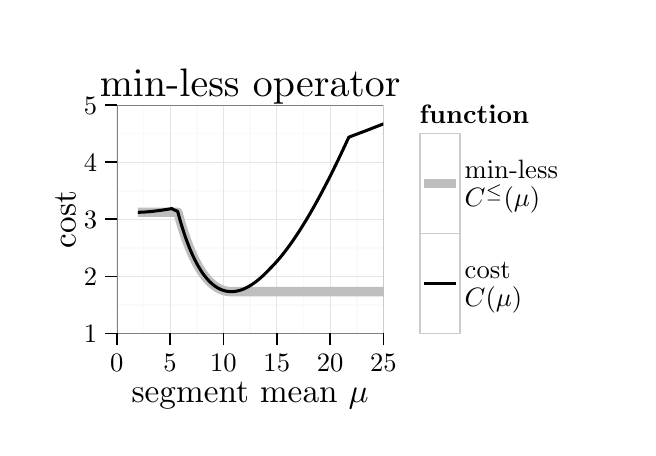
\begin{tikzpicture}[x=1pt,y=1pt]
\definecolor{fillColor}{RGB}{255,255,255}
\path[use as bounding box,fill=fillColor,fill opacity=0.00] (0,0) rectangle (216.81,144.54);
\begin{scope}
\path[clip] (  0.00,  0.00) rectangle (216.81,144.54);
\definecolor{drawColor}{RGB}{255,255,255}
\definecolor{fillColor}{RGB}{255,255,255}

\path[draw=drawColor,line width= 0.6pt,line join=round,line cap=round,fill=fillColor] (  0.00, -0.00) rectangle (216.81,144.54);
\end{scope}
\begin{scope}
\path[clip] ( 32.22, 34.03) rectangle (128.53,116.55);
\definecolor{fillColor}{RGB}{255,255,255}

\path[fill=fillColor] ( 32.22, 34.03) rectangle (128.53,116.55);
\definecolor{drawColor}{gray}{0.98}

\path[draw=drawColor,line width= 0.6pt,line join=round] ( 32.22, 44.35) --
	(128.53, 44.35);

\path[draw=drawColor,line width= 0.6pt,line join=round] ( 32.22, 64.98) --
	(128.53, 64.98);

\path[draw=drawColor,line width= 0.6pt,line join=round] ( 32.22, 85.61) --
	(128.53, 85.61);

\path[draw=drawColor,line width= 0.6pt,line join=round] ( 32.22,106.24) --
	(128.53,106.24);

\path[draw=drawColor,line width= 0.6pt,line join=round] ( 41.85, 34.03) --
	( 41.85,116.55);

\path[draw=drawColor,line width= 0.6pt,line join=round] ( 61.12, 34.03) --
	( 61.12,116.55);

\path[draw=drawColor,line width= 0.6pt,line join=round] ( 80.38, 34.03) --
	( 80.38,116.55);

\path[draw=drawColor,line width= 0.6pt,line join=round] ( 99.64, 34.03) --
	( 99.64,116.55);

\path[draw=drawColor,line width= 0.6pt,line join=round] (118.90, 34.03) --
	(118.90,116.55);
\definecolor{drawColor}{gray}{0.90}

\path[draw=drawColor,line width= 0.2pt,line join=round] ( 32.22, 34.03) --
	(128.53, 34.03);

\path[draw=drawColor,line width= 0.2pt,line join=round] ( 32.22, 54.66) --
	(128.53, 54.66);

\path[draw=drawColor,line width= 0.2pt,line join=round] ( 32.22, 75.29) --
	(128.53, 75.29);

\path[draw=drawColor,line width= 0.2pt,line join=round] ( 32.22, 95.92) --
	(128.53, 95.92);

\path[draw=drawColor,line width= 0.2pt,line join=round] ( 32.22,116.55) --
	(128.53,116.55);

\path[draw=drawColor,line width= 0.2pt,line join=round] ( 32.22, 34.03) --
	( 32.22,116.55);

\path[draw=drawColor,line width= 0.2pt,line join=round] ( 51.48, 34.03) --
	( 51.48,116.55);

\path[draw=drawColor,line width= 0.2pt,line join=round] ( 70.75, 34.03) --
	( 70.75,116.55);

\path[draw=drawColor,line width= 0.2pt,line join=round] ( 90.01, 34.03) --
	( 90.01,116.55);

\path[draw=drawColor,line width= 0.2pt,line join=round] (109.27, 34.03) --
	(109.27,116.55);

\path[draw=drawColor,line width= 0.2pt,line join=round] (128.53, 34.03) --
	(128.53,116.55);
\definecolor{drawColor}{RGB}{190,190,190}

\path[draw=drawColor,line width= 3.4pt,line join=round] ( 39.81, 77.83) --
	( 39.96, 77.83) --
	( 40.10, 77.83) --
	( 40.25, 77.83) --
	( 40.40, 77.83) --
	( 40.54, 77.83) --
	( 40.69, 77.83) --
	( 40.83, 77.83) --
	( 40.98, 77.83) --
	( 41.13, 77.83) --
	( 41.27, 77.83) --
	( 41.42, 77.83) --
	( 41.56, 77.83) --
	( 41.71, 77.83) --
	( 41.86, 77.83) --
	( 42.00, 77.83) --
	( 42.15, 77.83) --
	( 42.30, 77.83) --
	( 42.44, 77.83) --
	( 42.59, 77.83) --
	( 42.73, 77.83) --
	( 42.88, 77.83) --
	( 43.03, 77.83) --
	( 43.17, 77.83) --
	( 43.32, 77.83) --
	( 43.46, 77.83) --
	( 43.61, 77.83) --
	( 43.76, 77.83) --
	( 43.90, 77.83) --
	( 44.05, 77.83) --
	( 44.20, 77.83) --
	( 44.34, 77.83) --
	( 44.49, 77.83) --
	( 44.63, 77.83) --
	( 44.78, 77.83) --
	( 44.93, 77.83) --
	( 45.07, 77.83) --
	( 45.22, 77.83) --
	( 45.37, 77.83) --
	( 45.51, 77.83) --
	( 45.66, 77.83) --
	( 45.80, 77.83) --
	( 45.95, 77.83) --
	( 46.10, 77.83) --
	( 46.24, 77.83) --
	( 46.39, 77.83) --
	( 46.53, 77.83) --
	( 46.68, 77.83) --
	( 46.83, 77.83) --
	( 46.97, 77.83) --
	( 47.12, 77.83) --
	( 47.27, 77.83) --
	( 47.41, 77.83) --
	( 47.56, 77.83) --
	( 47.70, 77.83) --
	( 47.85, 77.83) --
	( 48.00, 77.83) --
	( 48.14, 77.83) --
	( 48.29, 77.83) --
	( 48.43, 77.83) --
	( 48.58, 77.83) --
	( 48.73, 77.83) --
	( 48.87, 77.83) --
	( 49.02, 77.83) --
	( 49.17, 77.83) --
	( 49.31, 77.83) --
	( 49.46, 77.83) --
	( 49.60, 77.83) --
	( 49.75, 77.83) --
	( 49.90, 77.83) --
	( 50.04, 77.83) --
	( 50.19, 77.83) --
	( 50.33, 77.83) --
	( 50.48, 77.83) --
	( 50.63, 77.83) --
	( 50.77, 77.83) --
	( 50.92, 77.83) --
	( 51.07, 77.83) --
	( 51.21, 77.83) --
	( 51.36, 77.83) --
	( 51.50, 77.83) --
	( 51.65, 77.83) --
	( 51.80, 77.83) --
	( 51.94, 77.83) --
	( 52.09, 77.83) --
	( 52.23, 77.83) --
	( 52.38, 77.83) --
	( 52.53, 77.83) --
	( 52.67, 77.83) --
	( 52.82, 77.83) --
	( 52.97, 77.83) --
	( 53.11, 77.83) --
	( 53.26, 77.83) --
	( 53.40, 77.83) --
	( 53.55, 77.83) --
	( 53.70, 77.83) --
	( 53.84, 77.83) --
	( 53.99, 77.83) --
	( 54.13, 77.83) --
	( 54.28, 77.83) --
	( 54.28, 77.83) --
	( 54.48, 77.11) --
	( 54.67, 76.40) --
	( 54.87, 75.70) --
	( 55.06, 75.02) --
	( 55.25, 74.35) --
	( 55.45, 73.69) --
	( 55.64, 73.05) --
	( 55.84, 72.41) --
	( 56.03, 71.79) --
	( 56.23, 71.18) --
	( 56.42, 70.58) --
	( 56.62, 70.00) --
	( 56.81, 69.42) --
	( 57.01, 68.86) --
	( 57.20, 68.31) --
	( 57.40, 67.77) --
	( 57.59, 67.24) --
	( 57.79, 66.72) --
	( 57.98, 66.20) --
	( 58.18, 65.70) --
	( 58.37, 65.21) --
	( 58.57, 64.73) --
	( 58.76, 64.26) --
	( 58.96, 63.80) --
	( 59.15, 63.35) --
	( 59.35, 62.91) --
	( 59.54, 62.47) --
	( 59.74, 62.05) --
	( 59.93, 61.64) --
	( 60.13, 61.23) --
	( 60.32, 60.83) --
	( 60.52, 60.44) --
	( 60.71, 60.06) --
	( 60.91, 59.69) --
	( 61.10, 59.32) --
	( 61.30, 58.97) --
	( 61.49, 58.62) --
	( 61.69, 58.28) --
	( 61.88, 57.94) --
	( 62.08, 57.62) --
	( 62.27, 57.30) --
	( 62.47, 56.99) --
	( 62.66, 56.69) --
	( 62.86, 56.39) --
	( 63.05, 56.10) --
	( 63.24, 55.82) --
	( 63.44, 55.55) --
	( 63.63, 55.28) --
	( 63.83, 55.02) --
	( 64.02, 54.77) --
	( 64.22, 54.52) --
	( 64.41, 54.28) --
	( 64.61, 54.04) --
	( 64.80, 53.81) --
	( 65.00, 53.59) --
	( 65.19, 53.38) --
	( 65.39, 53.17) --
	( 65.58, 52.97) --
	( 65.78, 52.77) --
	( 65.97, 52.58) --
	( 66.17, 52.39) --
	( 66.36, 52.21) --
	( 66.56, 52.04) --
	( 66.75, 51.87) --
	( 66.95, 51.71) --
	( 67.14, 51.55) --
	( 67.34, 51.40) --
	( 67.53, 51.26) --
	( 67.73, 51.12) --
	( 67.92, 50.98) --
	( 68.12, 50.85) --
	( 68.31, 50.73) --
	( 68.51, 50.61) --
	( 68.70, 50.50) --
	( 68.90, 50.39) --
	( 69.09, 50.28) --
	( 69.29, 50.18) --
	( 69.48, 50.09) --
	( 69.68, 50.00) --
	( 69.87, 49.92) --
	( 70.07, 49.84) --
	( 70.26, 49.76) --
	( 70.46, 49.69) --
	( 70.65, 49.62) --
	( 70.85, 49.56) --
	( 71.04, 49.51) --
	( 71.23, 49.45) --
	( 71.43, 49.41) --
	( 71.62, 49.36) --
	( 71.82, 49.32) --
	( 72.01, 49.29) --
	( 72.21, 49.26) --
	( 72.40, 49.23) --
	( 72.60, 49.21) --
	( 72.79, 49.19) --
	( 72.99, 49.18) --
	( 73.18, 49.17) --
	( 73.38, 49.16) --
	( 73.57, 49.16) --
	( 73.57, 49.16) --
	( 81.49, 49.16) --
	( 89.41, 49.16) --
	( 97.33, 49.16) --
	(105.25, 49.16) --
	(113.17, 49.16) --
	(121.09, 49.16) --
	(129.01, 49.16) --
	(136.93, 49.16) --
	(144.85, 49.16) --
	(152.77, 49.16) --
	(160.69, 49.16) --
	(168.60, 49.16) --
	(176.52, 49.16) --
	(184.44, 49.16) --
	(192.36, 49.16) --
	(200.28, 49.16) --
	(208.20, 49.16) --
	(216.12, 49.16) --
	(216.81, 49.16);
\definecolor{drawColor}{RGB}{0,0,0}

\path[draw=drawColor,line width= 1.1pt,line join=round] ( 39.81, 77.83) --
	( 39.94, 77.83) --
	( 40.06, 77.83) --
	( 40.18, 77.83) --
	( 40.31, 77.84) --
	( 40.43, 77.84) --
	( 40.55, 77.84) --
	( 40.68, 77.84) --
	( 40.80, 77.85) --
	( 40.93, 77.85) --
	( 41.05, 77.86) --
	( 41.17, 77.86) --
	( 41.30, 77.87) --
	( 41.42, 77.87) --
	( 41.55, 77.88) --
	( 41.67, 77.88) --
	( 41.79, 77.89) --
	( 41.92, 77.90) --
	( 42.04, 77.90) --
	( 42.17, 77.91) --
	( 42.29, 77.92) --
	( 42.41, 77.93) --
	( 42.54, 77.94) --
	( 42.66, 77.95) --
	( 42.79, 77.96) --
	( 42.91, 77.96) --
	( 43.03, 77.97) --
	( 43.16, 77.98) --
	( 43.28, 77.99) --
	( 43.41, 78.01) --
	( 43.53, 78.02) --
	( 43.65, 78.03) --
	( 43.78, 78.04) --
	( 43.90, 78.05) --
	( 44.03, 78.06) --
	( 44.15, 78.07) --
	( 44.27, 78.09) --
	( 44.40, 78.10) --
	( 44.52, 78.11) --
	( 44.65, 78.12) --
	( 44.77, 78.14) --
	( 44.89, 78.15) --
	( 45.02, 78.16) --
	( 45.14, 78.18) --
	( 45.26, 78.19) --
	( 45.39, 78.20) --
	( 45.51, 78.22) --
	( 45.64, 78.23) --
	( 45.76, 78.25) --
	( 45.88, 78.26) --
	( 46.01, 78.28) --
	( 46.13, 78.29) --
	( 46.26, 78.31) --
	( 46.38, 78.32) --
	( 46.50, 78.34) --
	( 46.63, 78.35) --
	( 46.75, 78.37) --
	( 46.88, 78.39) --
	( 47.00, 78.40) --
	( 47.12, 78.42) --
	( 47.25, 78.43) --
	( 47.37, 78.45) --
	( 47.50, 78.47) --
	( 47.62, 78.48) --
	( 47.74, 78.50) --
	( 47.87, 78.52) --
	( 47.99, 78.54) --
	( 48.12, 78.55) --
	( 48.24, 78.57) --
	( 48.36, 78.59) --
	( 48.49, 78.60) --
	( 48.61, 78.62) --
	( 48.74, 78.64) --
	( 48.86, 78.66) --
	( 48.98, 78.68) --
	( 49.11, 78.69) --
	( 49.23, 78.71) --
	( 49.36, 78.73) --
	( 49.48, 78.75) --
	( 49.60, 78.77) --
	( 49.73, 78.79) --
	( 49.85, 78.81) --
	( 49.98, 78.83) --
	( 50.10, 78.84) --
	( 50.22, 78.86) --
	( 50.35, 78.88) --
	( 50.47, 78.90) --
	( 50.59, 78.92) --
	( 50.72, 78.94) --
	( 50.84, 78.96) --
	( 50.97, 78.98) --
	( 51.09, 79.00) --
	( 51.21, 79.02) --
	( 51.34, 79.04) --
	( 51.46, 79.06) --
	( 51.59, 79.08) --
	( 51.71, 79.10) --
	( 51.83, 79.12) --
	( 51.96, 79.14) --
	( 52.08, 79.16) --
	( 52.08, 79.16) --
	( 52.10, 79.15) --
	( 52.12, 79.14) --
	( 52.15, 79.13) --
	( 52.17, 79.12) --
	( 52.19, 79.10) --
	( 52.21, 79.09) --
	( 52.23, 79.08) --
	( 52.25, 79.07) --
	( 52.27, 79.06) --
	( 52.30, 79.05) --
	( 52.32, 79.04) --
	( 52.34, 79.02) --
	( 52.36, 79.01) --
	( 52.38, 79.00) --
	( 52.40, 78.99) --
	( 52.42, 78.98) --
	( 52.44, 78.97) --
	( 52.47, 78.96) --
	( 52.49, 78.95) --
	( 52.51, 78.93) --
	( 52.53, 78.92) --
	( 52.55, 78.91) --
	( 52.57, 78.90) --
	( 52.59, 78.89) --
	( 52.61, 78.88) --
	( 52.64, 78.87) --
	( 52.66, 78.86) --
	( 52.68, 78.85) --
	( 52.70, 78.84) --
	( 52.72, 78.83) --
	( 52.74, 78.82) --
	( 52.76, 78.81) --
	( 52.78, 78.80) --
	( 52.81, 78.78) --
	( 52.83, 78.77) --
	( 52.85, 78.76) --
	( 52.87, 78.75) --
	( 52.89, 78.74) --
	( 52.91, 78.73) --
	( 52.93, 78.72) --
	( 52.96, 78.71) --
	( 52.98, 78.70) --
	( 53.00, 78.69) --
	( 53.02, 78.68) --
	( 53.04, 78.67) --
	( 53.06, 78.66) --
	( 53.08, 78.65) --
	( 53.10, 78.64) --
	( 53.13, 78.63) --
	( 53.15, 78.62) --
	( 53.17, 78.61) --
	( 53.19, 78.60) --
	( 53.21, 78.59) --
	( 53.23, 78.58) --
	( 53.25, 78.57) --
	( 53.27, 78.56) --
	( 53.30, 78.55) --
	( 53.32, 78.54) --
	( 53.34, 78.53) --
	( 53.36, 78.52) --
	( 53.38, 78.51) --
	( 53.40, 78.50) --
	( 53.42, 78.49) --
	( 53.44, 78.48) --
	( 53.47, 78.48) --
	( 53.49, 78.47) --
	( 53.51, 78.46) --
	( 53.53, 78.45) --
	( 53.55, 78.44) --
	( 53.57, 78.43) --
	( 53.59, 78.42) --
	( 53.62, 78.41) --
	( 53.64, 78.40) --
	( 53.66, 78.39) --
	( 53.68, 78.38) --
	( 53.70, 78.37) --
	( 53.72, 78.36) --
	( 53.74, 78.36) --
	( 53.76, 78.35) --
	( 53.79, 78.34) --
	( 53.81, 78.33) --
	( 53.83, 78.32) --
	( 53.85, 78.31) --
	( 53.87, 78.30) --
	( 53.89, 78.29) --
	( 53.91, 78.28) --
	( 53.93, 78.27) --
	( 53.96, 78.27) --
	( 53.98, 78.26) --
	( 54.00, 78.25) --
	( 54.02, 78.24) --
	( 54.04, 78.23) --
	( 54.06, 78.22) --
	( 54.08, 78.21) --
	( 54.10, 78.21) --
	( 54.13, 78.20) --
	( 54.15, 78.19) --
	( 54.17, 78.18) --
	( 54.19, 78.17) --
	( 54.19, 78.17) --
	( 54.53, 76.92) --
	( 54.87, 75.70) --
	( 55.20, 74.52) --
	( 55.54, 73.38) --
	( 55.88, 72.28) --
	( 56.22, 71.22) --
	( 56.56, 70.19) --
	( 56.89, 69.19) --
	( 57.23, 68.23) --
	( 57.57, 67.30) --
	( 57.91, 66.40) --
	( 58.24, 65.54) --
	( 58.58, 64.70) --
	( 58.92, 63.89) --
	( 59.26, 63.11) --
	( 59.60, 62.36) --
	( 59.93, 61.63) --
	( 60.27, 60.93) --
	( 60.61, 60.26) --
	( 60.95, 59.61) --
	( 61.29, 58.98) --
	( 61.62, 58.38) --
	( 61.96, 57.81) --
	( 62.30, 57.25) --
	( 62.64, 56.72) --
	( 62.98, 56.21) --
	( 63.31, 55.72) --
	( 63.65, 55.26) --
	( 63.99, 54.81) --
	( 64.33, 54.38) --
	( 64.67, 53.98) --
	( 65.00, 53.59) --
	( 65.34, 53.22) --
	( 65.68, 52.87) --
	( 66.02, 52.54) --
	( 66.35, 52.22) --
	( 66.69, 51.92) --
	( 67.03, 51.64) --
	( 67.37, 51.38) --
	( 67.71, 51.13) --
	( 68.04, 50.90) --
	( 68.38, 50.68) --
	( 68.72, 50.48) --
	( 69.06, 50.30) --
	( 69.40, 50.13) --
	( 69.73, 49.97) --
	( 70.07, 49.83) --
	( 70.41, 49.71) --
	( 70.75, 49.59) --
	( 71.09, 49.49) --
	( 71.42, 49.41) --
	( 71.76, 49.34) --
	( 72.10, 49.28) --
	( 72.44, 49.23) --
	( 72.78, 49.19) --
	( 73.11, 49.17) --
	( 73.45, 49.16) --
	( 73.79, 49.16) --
	( 74.13, 49.18) --
	( 74.46, 49.20) --
	( 74.80, 49.24) --
	( 75.14, 49.28) --
	( 75.48, 49.34) --
	( 75.82, 49.41) --
	( 76.15, 49.49) --
	( 76.49, 49.58) --
	( 76.83, 49.68) --
	( 77.17, 49.79) --
	( 77.51, 49.91) --
	( 77.84, 50.04) --
	( 78.18, 50.18) --
	( 78.52, 50.33) --
	( 78.86, 50.49) --
	( 79.20, 50.66) --
	( 79.53, 50.84) --
	( 79.87, 51.03) --
	( 80.21, 51.22) --
	( 80.55, 51.43) --
	( 80.89, 51.64) --
	( 81.22, 51.86) --
	( 81.56, 52.09) --
	( 81.90, 52.33) --
	( 82.24, 52.58) --
	( 82.57, 52.83) --
	( 82.91, 53.10) --
	( 83.25, 53.37) --
	( 83.59, 53.64) --
	( 83.93, 53.93) --
	( 84.26, 54.22) --
	( 84.60, 54.53) --
	( 84.94, 54.83) --
	( 85.28, 55.15) --
	( 85.62, 55.47) --
	( 85.95, 55.80) --
	( 86.29, 56.14) --
	( 86.63, 56.48) --
	( 86.97, 56.83) --
	( 87.31, 57.19) --
	( 87.64, 57.56) --
	( 87.64, 57.56) --
	( 87.93, 57.84) --
	( 88.22, 58.13) --
	( 88.50, 58.43) --
	( 88.79, 58.73) --
	( 89.08, 59.03) --
	( 89.36, 59.34) --
	( 89.65, 59.66) --
	( 89.94, 59.98) --
	( 90.22, 60.30) --
	( 90.51, 60.63) --
	( 90.80, 60.96) --
	( 91.09, 61.30) --
	( 91.37, 61.65) --
	( 91.66, 62.00) --
	( 91.95, 62.35) --
	( 92.23, 62.71) --
	( 92.52, 63.07) --
	( 92.81, 63.44) --
	( 93.09, 63.81) --
	( 93.38, 64.18) --
	( 93.67, 64.56) --
	( 93.95, 64.95) --
	( 94.24, 65.34) --
	( 94.53, 65.73) --
	( 94.81, 66.13) --
	( 95.10, 66.53) --
	( 95.39, 66.93) --
	( 95.67, 67.34) --
	( 95.96, 67.76) --
	( 96.25, 68.17) --
	( 96.53, 68.59) --
	( 96.82, 69.02) --
	( 97.11, 69.45) --
	( 97.39, 69.88) --
	( 97.68, 70.32) --
	( 97.97, 70.76) --
	( 98.25, 71.20) --
	( 98.54, 71.65) --
	( 98.83, 72.10) --
	( 99.11, 72.56) --
	( 99.40, 73.02) --
	( 99.69, 73.48) --
	( 99.98, 73.95) --
	(100.26, 74.42) --
	(100.55, 74.89) --
	(100.84, 75.37) --
	(101.12, 75.85) --
	(101.41, 76.33) --
	(101.70, 76.82) --
	(101.98, 77.31) --
	(102.27, 77.80) --
	(102.56, 78.30) --
	(102.84, 78.80) --
	(103.13, 79.31) --
	(103.42, 79.81) --
	(103.70, 80.32) --
	(103.99, 80.84) --
	(104.28, 81.35) --
	(104.56, 81.87) --
	(104.85, 82.39) --
	(105.14, 82.92) --
	(105.42, 83.45) --
	(105.71, 83.98) --
	(106.00, 84.52) --
	(106.28, 85.05) --
	(106.57, 85.60) --
	(106.86, 86.14) --
	(107.14, 86.69) --
	(107.43, 87.24) --
	(107.72, 87.79) --
	(108.01, 88.34) --
	(108.29, 88.90) --
	(108.58, 89.46) --
	(108.87, 90.03) --
	(109.15, 90.59) --
	(109.44, 91.16) --
	(109.73, 91.73) --
	(110.01, 92.31) --
	(110.30, 92.89) --
	(110.59, 93.47) --
	(110.87, 94.05) --
	(111.16, 94.64) --
	(111.45, 95.22) --
	(111.73, 95.81) --
	(112.02, 96.41) --
	(112.31, 97.00) --
	(112.59, 97.60) --
	(112.88, 98.20) --
	(113.17, 98.81) --
	(113.45, 99.41) --
	(113.74,100.02) --
	(114.03,100.63) --
	(114.31,101.24) --
	(114.60,101.86) --
	(114.89,102.48) --
	(115.17,103.10) --
	(115.46,103.72) --
	(115.75,104.34) --
	(116.04,104.97) --
	(116.04,104.97) --
	(123.53,107.81) --
	(131.02,110.74) --
	(138.51,113.74) --
	(146.00,116.82) --
	(153.49,119.96) --
	(160.98,123.14) --
	(168.47,126.38) --
	(175.96,129.66) --
	(183.45,132.97) --
	(190.94,136.32) --
	(198.43,139.69) --
	(205.92,143.10) --
	(209.06,144.54);
\definecolor{drawColor}{gray}{0.50}

\path[draw=drawColor,line width= 0.6pt,line join=round,line cap=round] ( 32.22, 34.03) rectangle (128.53,116.55);
\end{scope}
\begin{scope}
\path[clip] (  0.00,  0.00) rectangle (216.81,144.54);
\definecolor{drawColor}{RGB}{0,0,0}

\node[text=drawColor,anchor=base east,inner sep=0pt, outer sep=0pt, scale=  0.96] at ( 25.11, 30.73) {1};

\node[text=drawColor,anchor=base east,inner sep=0pt, outer sep=0pt, scale=  0.96] at ( 25.11, 51.36) {2};

\node[text=drawColor,anchor=base east,inner sep=0pt, outer sep=0pt, scale=  0.96] at ( 25.11, 71.99) {3};

\node[text=drawColor,anchor=base east,inner sep=0pt, outer sep=0pt, scale=  0.96] at ( 25.11, 92.62) {4};

\node[text=drawColor,anchor=base east,inner sep=0pt, outer sep=0pt, scale=  0.96] at ( 25.11,113.25) {5};
\end{scope}
\begin{scope}
\path[clip] (  0.00,  0.00) rectangle (216.81,144.54);
\definecolor{drawColor}{RGB}{0,0,0}

\path[draw=drawColor,line width= 0.6pt,line join=round] ( 27.95, 34.03) --
	( 32.22, 34.03);

\path[draw=drawColor,line width= 0.6pt,line join=round] ( 27.95, 54.66) --
	( 32.22, 54.66);

\path[draw=drawColor,line width= 0.6pt,line join=round] ( 27.95, 75.29) --
	( 32.22, 75.29);

\path[draw=drawColor,line width= 0.6pt,line join=round] ( 27.95, 95.92) --
	( 32.22, 95.92);

\path[draw=drawColor,line width= 0.6pt,line join=round] ( 27.95,116.55) --
	( 32.22,116.55);
\end{scope}
\begin{scope}
\path[clip] (  0.00,  0.00) rectangle (216.81,144.54);
\definecolor{drawColor}{RGB}{0,0,0}

\path[draw=drawColor,line width= 0.6pt,line join=round] ( 32.22, 29.77) --
	( 32.22, 34.03);

\path[draw=drawColor,line width= 0.6pt,line join=round] ( 51.48, 29.77) --
	( 51.48, 34.03);

\path[draw=drawColor,line width= 0.6pt,line join=round] ( 70.75, 29.77) --
	( 70.75, 34.03);

\path[draw=drawColor,line width= 0.6pt,line join=round] ( 90.01, 29.77) --
	( 90.01, 34.03);

\path[draw=drawColor,line width= 0.6pt,line join=round] (109.27, 29.77) --
	(109.27, 34.03);

\path[draw=drawColor,line width= 0.6pt,line join=round] (128.53, 29.77) --
	(128.53, 34.03);
\end{scope}
\begin{scope}
\path[clip] (  0.00,  0.00) rectangle (216.81,144.54);
\definecolor{drawColor}{RGB}{0,0,0}

\node[text=drawColor,anchor=base,inner sep=0pt, outer sep=0pt, scale=  0.96] at ( 32.22, 20.31) {0};

\node[text=drawColor,anchor=base,inner sep=0pt, outer sep=0pt, scale=  0.96] at ( 51.48, 20.31) {5};

\node[text=drawColor,anchor=base,inner sep=0pt, outer sep=0pt, scale=  0.96] at ( 70.75, 20.31) {10};

\node[text=drawColor,anchor=base,inner sep=0pt, outer sep=0pt, scale=  0.96] at ( 90.01, 20.31) {15};

\node[text=drawColor,anchor=base,inner sep=0pt, outer sep=0pt, scale=  0.96] at (109.27, 20.31) {20};

\node[text=drawColor,anchor=base,inner sep=0pt, outer sep=0pt, scale=  0.96] at (128.53, 20.31) {25};
\end{scope}
\begin{scope}
\path[clip] (  0.00,  0.00) rectangle (216.81,144.54);
\definecolor{drawColor}{RGB}{0,0,0}

\node[text=drawColor,anchor=base,inner sep=0pt, outer sep=0pt, scale=  1.20] at ( 80.38,  9.03) {segment mean $\mu$};
\end{scope}
\begin{scope}
\path[clip] (  0.00,  0.00) rectangle (216.81,144.54);
\definecolor{drawColor}{RGB}{0,0,0}

\node[text=drawColor,rotate= 90.00,anchor=base,inner sep=0pt, outer sep=0pt, scale=  1.20] at ( 17.30, 75.29) {cost};
\end{scope}
\begin{scope}
\path[clip] (  0.00,  0.00) rectangle (216.81,144.54);
\definecolor{fillColor}{RGB}{255,255,255}

\path[fill=fillColor] (137.40, 29.77) rectangle (195.90,120.82);
\end{scope}
\begin{scope}
\path[clip] (  0.00,  0.00) rectangle (216.81,144.54);
\definecolor{drawColor}{RGB}{0,0,0}

\node[text=drawColor,anchor=base west,inner sep=0pt, outer sep=0pt, scale=  0.96] at (141.67,109.92) {\bfseries function};
\end{scope}
\begin{scope}
\path[clip] (  0.00,  0.00) rectangle (216.81,144.54);
\definecolor{drawColor}{gray}{0.80}
\definecolor{fillColor}{RGB}{255,255,255}

\path[draw=drawColor,line width= 0.6pt,line join=round,line cap=round,fill=fillColor] (141.67, 70.18) rectangle (156.12,106.31);
\end{scope}
\begin{scope}
\path[clip] (  0.00,  0.00) rectangle (216.81,144.54);
\definecolor{drawColor}{RGB}{190,190,190}

\path[draw=drawColor,line width= 3.4pt,line join=round] (143.12, 88.24) -- (154.68, 88.24);
\end{scope}
\begin{scope}
\path[clip] (  0.00,  0.00) rectangle (216.81,144.54);
\definecolor{drawColor}{gray}{0.80}
\definecolor{fillColor}{RGB}{255,255,255}

\path[draw=drawColor,line width= 0.6pt,line join=round,line cap=round,fill=fillColor] (141.67, 34.04) rectangle (156.12, 70.18);
\end{scope}
\begin{scope}
\path[clip] (  0.00,  0.00) rectangle (216.81,144.54);
\definecolor{drawColor}{RGB}{0,0,0}

\path[draw=drawColor,line width= 1.1pt,line join=round] (143.12, 52.11) -- (154.68, 52.11);
\end{scope}
\begin{scope}
\path[clip] (  0.00,  0.00) rectangle (216.81,144.54);
\definecolor{drawColor}{RGB}{0,0,0}

\node[text=drawColor,anchor=base west,inner sep=0pt, outer sep=0pt, scale=  0.96] at (157.93, 90.12) {min-less};

\node[text=drawColor,anchor=base west,inner sep=0pt, outer sep=0pt, scale=  0.96] at (157.93, 79.75) {$C^{\leq}(\mu)$};
\end{scope}
\begin{scope}
\path[clip] (  0.00,  0.00) rectangle (216.81,144.54);
\definecolor{drawColor}{RGB}{0,0,0}

\node[text=drawColor,anchor=base west,inner sep=0pt, outer sep=0pt, scale=  0.96] at (157.93, 53.99) {cost};

\node[text=drawColor,anchor=base west,inner sep=0pt, outer sep=0pt, scale=  0.96] at (157.93, 43.62) {$C(\mu)$};
\end{scope}
\begin{scope}
\path[clip] (  0.00,  0.00) rectangle (216.81,144.54);
\definecolor{drawColor}{RGB}{0,0,0}

\node[text=drawColor,anchor=base,inner sep=0pt, outer sep=0pt, scale=  1.44] at ( 80.38,119.57) {min-less operator};
\end{scope}
\end{tikzpicture}

    \end{center}
  }
  \caption{\label{fig:min-operators} \textbf{Left:} The min-more
    operator is $C^{\geq}(\mu)=\min_{x\geq \mu}C(x)$. \textbf{Right:}
    The min-less operator is $C^{\leq}(\mu)=\min_{x\leq
      \mu}C(x)$.}
\end{figure}

The next step is to compute the minimum cost in 2 segments up to data
point 3, for which there is a choice of two change-points.
\begin{equation*}
  \FCC_{2,3}(\mu) = \min
  \begin{cases}
    \FCC_{2,2}(\mu)+\gamma_3(\mu), \\
    \FCC_{1,2}^{\leq}(\mu)+\gamma_3(\mu)
  \end{cases}
\end{equation*}
We have already computed an exact representation of the $C_{2,2}$
term, which is the cost a change after the first data point. Now we
need to compare it with the $C_{1,2}^{\leq}$ term, which is the cost
of a change after the second data point. This is a crucial step in
which the \texttt{MinEnvelope} sub-routine computes an exact
representation of the minimum of these two functions
(Figure~\ref{fig:min-envelope}).

\begin{figure}[!t]
  \begin{center}
    % Created by tikzDevice version 0.10.1 on 2017-02-20 09:55:27
% !TEX encoding = UTF-8 Unicode
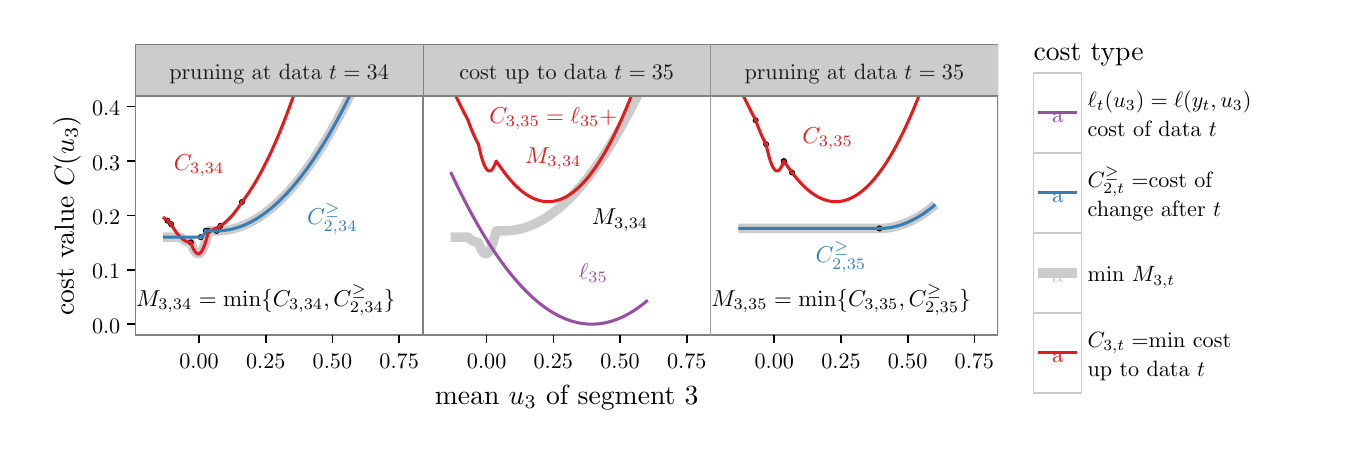
\begin{tikzpicture}[x=1pt,y=1pt]
\definecolor{fillColor}{RGB}{255,255,255}
\path[use as bounding box,fill=fillColor,fill opacity=0.00] (0,0) rectangle (469.75,144.54);
\begin{scope}
\path[clip] (  0.00,  0.00) rectangle (469.75,144.54);
\definecolor{drawColor}{RGB}{255,255,255}
\definecolor{fillColor}{RGB}{255,255,255}

\path[draw=drawColor,line width= 0.6pt,line join=round,line cap=round,fill=fillColor] (  0.00, -0.00) rectangle (469.76,144.54);
\end{scope}
\begin{scope}
\path[clip] ( 38.87,119.93) rectangle (142.81,138.54);
\definecolor{drawColor}{gray}{0.50}
\definecolor{fillColor}{gray}{0.80}

\path[draw=drawColor,line width= 0.2pt,line join=round,line cap=round,fill=fillColor] ( 38.87,119.93) rectangle (142.81,138.54);
\definecolor{drawColor}{gray}{0.10}

\node[text=drawColor,anchor=base,inner sep=0pt, outer sep=0pt, scale=  0.80] at ( 90.84,125.93) {pruning at data $t=34$};
\end{scope}
\begin{scope}
\path[clip] (142.81,119.93) rectangle (246.74,138.54);
\definecolor{drawColor}{gray}{0.50}
\definecolor{fillColor}{gray}{0.80}

\path[draw=drawColor,line width= 0.2pt,line join=round,line cap=round,fill=fillColor] (142.81,119.93) rectangle (246.74,138.54);
\definecolor{drawColor}{gray}{0.10}

\node[text=drawColor,anchor=base,inner sep=0pt, outer sep=0pt, scale=  0.80] at (194.77,125.93) {cost up to data $t=35$};
\end{scope}
\begin{scope}
\path[clip] (246.74,119.93) rectangle (350.67,138.54);
\definecolor{drawColor}{gray}{0.50}
\definecolor{fillColor}{gray}{0.80}

\path[draw=drawColor,line width= 0.2pt,line join=round,line cap=round,fill=fillColor] (246.74,119.93) rectangle (350.67,138.54);
\definecolor{drawColor}{gray}{0.10}

\node[text=drawColor,anchor=base,inner sep=0pt, outer sep=0pt, scale=  0.80] at (298.71,125.93) {pruning at data $t=35$};
\end{scope}
\begin{scope}
\path[clip] ( 38.87, 33.48) rectangle (142.81,119.93);
\definecolor{fillColor}{RGB}{255,255,255}

\path[fill=fillColor] ( 38.87, 33.48) rectangle (142.81,119.93);
\definecolor{drawColor}{gray}{0.80}

\path[draw=drawColor,line width= 3.4pt,line join=round] ( 48.91, 68.84) --
	( 48.98, 68.84) --
	( 49.04, 68.84) --
	( 49.10, 68.84) --
	( 49.17, 68.84) --
	( 49.23, 68.84) --
	( 49.29, 68.84) --
	( 49.36, 68.84) --
	( 49.42, 68.84) --
	( 49.48, 68.84) --
	( 49.55, 68.84) --
	( 49.61, 68.84) --
	( 49.67, 68.84) --
	( 49.74, 68.84) --
	( 49.80, 68.84) --
	( 49.86, 68.84) --
	( 49.93, 68.84) --
	( 49.99, 68.84) --
	( 50.06, 68.84) --
	( 50.12, 68.84) --
	( 50.18, 68.84) --
	( 50.25, 68.84) --
	( 50.31, 68.84) --
	( 50.37, 68.84) --
	( 50.44, 68.84) --
	( 50.50, 68.84) --
	( 50.56, 68.84) --
	( 50.63, 68.84) --
	( 50.69, 68.84) --
	( 50.75, 68.84) --
	( 50.82, 68.84) --
	( 50.88, 68.84) --
	( 50.94, 68.84) --
	( 51.01, 68.84) --
	( 51.07, 68.84) --
	( 51.14, 68.84) --
	( 51.20, 68.84) --
	( 51.26, 68.84) --
	( 51.33, 68.84) --
	( 51.39, 68.84) --
	( 51.45, 68.84) --
	( 51.52, 68.84) --
	( 51.58, 68.84) --
	( 51.64, 68.84) --
	( 51.71, 68.84) --
	( 51.77, 68.84) --
	( 51.83, 68.84) --
	( 51.90, 68.84) --
	( 51.96, 68.84) --
	( 52.02, 68.84) --
	( 52.09, 68.84) --
	( 52.15, 68.84) --
	( 52.22, 68.84) --
	( 52.28, 68.84) --
	( 52.34, 68.84) --
	( 52.41, 68.84) --
	( 52.47, 68.84) --
	( 52.53, 68.84) --
	( 52.60, 68.84) --
	( 52.66, 68.84) --
	( 52.72, 68.84) --
	( 52.79, 68.84) --
	( 52.85, 68.84) --
	( 52.91, 68.84) --
	( 52.98, 68.84) --
	( 53.04, 68.84) --
	( 53.10, 68.84) --
	( 53.17, 68.84) --
	( 53.23, 68.84) --
	( 53.30, 68.84) --
	( 53.36, 68.84) --
	( 53.42, 68.84) --
	( 53.49, 68.84) --
	( 53.55, 68.84) --
	( 53.61, 68.84) --
	( 53.68, 68.84) --
	( 53.74, 68.84) --
	( 53.80, 68.84) --
	( 53.87, 68.84) --
	( 53.93, 68.84) --
	( 53.99, 68.84) --
	( 54.06, 68.84) --
	( 54.12, 68.84) --
	( 54.18, 68.84) --
	( 54.25, 68.84) --
	( 54.31, 68.84) --
	( 54.38, 68.84) --
	( 54.44, 68.84) --
	( 54.50, 68.84) --
	( 54.57, 68.84) --
	( 54.63, 68.84) --
	( 54.69, 68.84) --
	( 54.76, 68.84) --
	( 54.82, 68.84) --
	( 54.88, 68.84) --
	( 54.95, 68.84) --
	( 55.01, 68.84) --
	( 55.07, 68.84) --
	( 55.14, 68.84) --
	( 55.20, 68.84) --
	( 55.20, 68.84) --
	( 55.24, 68.80) --
	( 55.28, 68.76) --
	( 55.32, 68.73) --
	( 55.35, 68.69) --
	( 55.39, 68.66) --
	( 55.43, 68.62) --
	( 55.47, 68.59) --
	( 55.51, 68.55) --
	( 55.54, 68.52) --
	( 55.58, 68.48) --
	( 55.62, 68.45) --
	( 55.66, 68.42) --
	( 55.69, 68.39) --
	( 55.73, 68.35) --
	( 55.77, 68.32) --
	( 55.81, 68.29) --
	( 55.85, 68.26) --
	( 55.88, 68.23) --
	( 55.92, 68.20) --
	( 55.96, 68.17) --
	( 56.00, 68.14) --
	( 56.04, 68.11) --
	( 56.07, 68.08) --
	( 56.11, 68.05) --
	( 56.15, 68.02) --
	( 56.19, 68.00) --
	( 56.23, 67.97) --
	( 56.26, 67.94) --
	( 56.30, 67.92) --
	( 56.34, 67.89) --
	( 56.38, 67.86) --
	( 56.42, 67.84) --
	( 56.45, 67.81) --
	( 56.49, 67.79) --
	( 56.53, 67.76) --
	( 56.57, 67.74) --
	( 56.61, 67.72) --
	( 56.64, 67.69) --
	( 56.68, 67.67) --
	( 56.72, 67.65) --
	( 56.76, 67.62) --
	( 56.80, 67.60) --
	( 56.83, 67.58) --
	( 56.87, 67.56) --
	( 56.91, 67.54) --
	( 56.95, 67.52) --
	( 56.99, 67.50) --
	( 57.02, 67.48) --
	( 57.06, 67.46) --
	( 57.10, 67.44) --
	( 57.14, 67.42) --
	( 57.17, 67.40) --
	( 57.21, 67.39) --
	( 57.25, 67.37) --
	( 57.29, 67.35) --
	( 57.33, 67.33) --
	( 57.36, 67.32) --
	( 57.40, 67.30) --
	( 57.44, 67.29) --
	( 57.48, 67.27) --
	( 57.52, 67.26) --
	( 57.55, 67.24) --
	( 57.59, 67.23) --
	( 57.63, 67.21) --
	( 57.67, 67.20) --
	( 57.71, 67.19) --
	( 57.74, 67.17) --
	( 57.78, 67.16) --
	( 57.82, 67.15) --
	( 57.86, 67.14) --
	( 57.90, 67.13) --
	( 57.93, 67.11) --
	( 57.97, 67.10) --
	( 58.01, 67.09) --
	( 58.05, 67.08) --
	( 58.09, 67.07) --
	( 58.12, 67.07) --
	( 58.16, 67.06) --
	( 58.20, 67.05) --
	( 58.24, 67.04) --
	( 58.28, 67.03) --
	( 58.31, 67.03) --
	( 58.35, 67.02) --
	( 58.39, 67.01) --
	( 58.43, 67.01) --
	( 58.47, 67.00) --
	( 58.50, 66.99) --
	( 58.54, 66.99) --
	( 58.58, 66.98) --
	( 58.62, 66.98) --
	( 58.65, 66.98) --
	( 58.69, 66.97) --
	( 58.73, 66.97) --
	( 58.77, 66.97) --
	( 58.81, 66.96) --
	( 58.84, 66.96) --
	( 58.88, 66.96) --
	( 58.92, 66.96) --
	( 58.96, 66.96) --
	( 58.96, 66.96) --
	( 59.02, 66.76) --
	( 59.09, 66.56) --
	( 59.15, 66.38) --
	( 59.22, 66.19) --
	( 59.28, 66.01) --
	( 59.34, 65.84) --
	( 59.41, 65.67) --
	( 59.47, 65.50) --
	( 59.54, 65.34) --
	( 59.60, 65.19) --
	( 59.67, 65.04) --
	( 59.73, 64.89) --
	( 59.80, 64.75) --
	( 59.86, 64.62) --
	( 59.92, 64.49) --
	( 59.99, 64.36) --
	( 60.05, 64.24) --
	( 60.12, 64.13) --
	( 60.18, 64.02) --
	( 60.25, 63.91) --
	( 60.31, 63.81) --
	( 60.38, 63.72) --
	( 60.44, 63.62) --
	( 60.50, 63.54) --
	( 60.57, 63.46) --
	( 60.63, 63.38) --
	( 60.70, 63.31) --
	( 60.76, 63.24) --
	( 60.83, 63.18) --
	( 60.89, 63.12) --
	( 60.95, 63.07) --
	( 61.02, 63.03) --
	( 61.08, 62.98) --
	( 61.15, 62.95) --
	( 61.21, 62.92) --
	( 61.28, 62.89) --
	( 61.34, 62.87) --
	( 61.41, 62.85) --
	( 61.47, 62.84) --
	( 61.53, 62.83) --
	( 61.60, 62.83) --
	( 61.66, 62.83) --
	( 61.73, 62.84) --
	( 61.79, 62.85) --
	( 61.86, 62.86) --
	( 61.92, 62.89) --
	( 61.98, 62.91) --
	( 62.05, 62.95) --
	( 62.11, 62.98) --
	( 62.18, 63.02) --
	( 62.24, 63.07) --
	( 62.31, 63.12) --
	( 62.37, 63.18) --
	( 62.44, 63.24) --
	( 62.50, 63.30) --
	( 62.56, 63.38) --
	( 62.63, 63.45) --
	( 62.69, 63.53) --
	( 62.76, 63.62) --
	( 62.82, 63.71) --
	( 62.89, 63.80) --
	( 62.95, 63.90) --
	( 63.01, 64.01) --
	( 63.08, 64.12) --
	( 63.14, 64.24) --
	( 63.21, 64.36) --
	( 63.27, 64.48) --
	( 63.34, 64.61) --
	( 63.40, 64.75) --
	( 63.47, 64.88) --
	( 63.53, 65.03) --
	( 63.59, 65.18) --
	( 63.66, 65.33) --
	( 63.72, 65.49) --
	( 63.79, 65.66) --
	( 63.85, 65.83) --
	( 63.92, 66.00) --
	( 63.98, 66.18) --
	( 64.05, 66.36) --
	( 64.11, 66.55) --
	( 64.17, 66.75) --
	( 64.24, 66.94) --
	( 64.30, 67.15) --
	( 64.37, 67.36) --
	( 64.43, 67.57) --
	( 64.50, 67.79) --
	( 64.56, 68.01) --
	( 64.62, 68.24) --
	( 64.69, 68.47) --
	( 64.75, 68.71) --
	( 64.82, 68.95) --
	( 64.88, 69.20) --
	( 64.95, 69.45) --
	( 65.01, 69.71) --
	( 65.08, 69.97) --
	( 65.14, 70.24) --
	( 65.20, 70.51) --
	( 65.27, 70.79) --
	( 65.33, 71.07) --
	( 65.33, 71.07) --
	( 65.33, 71.07) --
	( 65.34, 71.07) --
	( 65.34, 71.07) --
	( 65.34, 71.07) --
	( 65.34, 71.07) --
	( 65.35, 71.07) --
	( 65.35, 71.07) --
	( 65.35, 71.07) --
	( 65.35, 71.08) --
	( 65.35, 71.08) --
	( 65.36, 71.08) --
	( 65.36, 71.08) --
	( 65.36, 71.08) --
	( 65.36, 71.08) --
	( 65.36, 71.08) --
	( 65.37, 71.08) --
	( 65.37, 71.08) --
	( 65.37, 71.08) --
	( 65.37, 71.08) --
	( 65.37, 71.08) --
	( 65.38, 71.08) --
	( 65.38, 71.08) --
	( 65.38, 71.08) --
	( 65.38, 71.08) --
	( 65.38, 71.08) --
	( 65.39, 71.08) --
	( 65.39, 71.08) --
	( 65.39, 71.08) --
	( 65.39, 71.09) --
	( 65.39, 71.09) --
	( 65.40, 71.09) --
	( 65.40, 71.09) --
	( 65.40, 71.09) --
	( 65.40, 71.09) --
	( 65.40, 71.09) --
	( 65.41, 71.09) --
	( 65.41, 71.09) --
	( 65.41, 71.09) --
	( 65.41, 71.09) --
	( 65.41, 71.09) --
	( 65.42, 71.09) --
	( 65.42, 71.09) --
	( 65.42, 71.09) --
	( 65.42, 71.09) --
	( 65.42, 71.09) --
	( 65.43, 71.09) --
	( 65.43, 71.09) --
	( 65.43, 71.10) --
	( 65.43, 71.10) --
	( 65.43, 71.10) --
	( 65.44, 71.10) --
	( 65.44, 71.10) --
	( 65.44, 71.10) --
	( 65.44, 71.10) --
	( 65.44, 71.10) --
	( 65.45, 71.10) --
	( 65.45, 71.10) --
	( 65.45, 71.10) --
	( 65.45, 71.10) --
	( 65.46, 71.10) --
	( 65.46, 71.10) --
	( 65.46, 71.10) --
	( 65.46, 71.10) --
	( 65.46, 71.10) --
	( 65.47, 71.10) --
	( 65.47, 71.10) --
	( 65.47, 71.11) --
	( 65.47, 71.11) --
	( 65.47, 71.11) --
	( 65.48, 71.11) --
	( 65.48, 71.11) --
	( 65.48, 71.11) --
	( 65.48, 71.11) --
	( 65.48, 71.11) --
	( 65.49, 71.11) --
	( 65.49, 71.11) --
	( 65.49, 71.11) --
	( 65.49, 71.11) --
	( 65.49, 71.11) --
	( 65.50, 71.11) --
	( 65.50, 71.11) --
	( 65.50, 71.11) --
	( 65.50, 71.11) --
	( 65.50, 71.11) --
	( 65.51, 71.11) --
	( 65.51, 71.12) --
	( 65.51, 71.12) --
	( 65.51, 71.12) --
	( 65.51, 71.12) --
	( 65.52, 71.12) --
	( 65.52, 71.12) --
	( 65.52, 71.12) --
	( 65.52, 71.12) --
	( 65.52, 71.12) --
	( 65.53, 71.12) --
	( 65.53, 71.12) --
	( 65.53, 71.12) --
	( 65.53, 71.12) --
	( 65.53, 71.12) --
	( 65.53, 71.12) --
	( 65.56, 71.12) --
	( 65.59, 71.12) --
	( 65.62, 71.12) --
	( 65.65, 71.12) --
	( 65.68, 71.12) --
	( 65.70, 71.12) --
	( 65.73, 71.12) --
	( 65.76, 71.12) --
	( 65.79, 71.12) --
	( 65.82, 71.12) --
	( 65.84, 71.12) --
	( 65.87, 71.12) --
	( 65.90, 71.12) --
	( 65.93, 71.12) --
	( 65.96, 71.12) --
	( 65.98, 71.12) --
	( 66.01, 71.12) --
	( 66.04, 71.12) --
	( 66.07, 71.12) --
	( 66.10, 71.12) --
	( 66.13, 71.12) --
	( 66.15, 71.12) --
	( 66.18, 71.12) --
	( 66.21, 71.12) --
	( 66.24, 71.12) --
	( 66.27, 71.12) --
	( 66.29, 71.12) --
	( 66.32, 71.12) --
	( 66.35, 71.12) --
	( 66.38, 71.12) --
	( 66.41, 71.12) --
	( 66.43, 71.12) --
	( 66.46, 71.12) --
	( 66.49, 71.12) --
	( 66.52, 71.12) --
	( 66.55, 71.12) --
	( 66.58, 71.12) --
	( 66.60, 71.12) --
	( 66.63, 71.12) --
	( 66.66, 71.12) --
	( 66.69, 71.12) --
	( 66.72, 71.12) --
	( 66.74, 71.12) --
	( 66.77, 71.12) --
	( 66.80, 71.12) --
	( 66.83, 71.12) --
	( 66.86, 71.12) --
	( 66.89, 71.12) --
	( 66.91, 71.12) --
	( 66.94, 71.12) --
	( 66.97, 71.12) --
	( 67.00, 71.12) --
	( 67.03, 71.12) --
	( 67.05, 71.12) --
	( 67.08, 71.12) --
	( 67.11, 71.12) --
	( 67.14, 71.12) --
	( 67.17, 71.12) --
	( 67.19, 71.12) --
	( 67.22, 71.12) --
	( 67.25, 71.12) --
	( 67.28, 71.12) --
	( 67.31, 71.12) --
	( 67.34, 71.12) --
	( 67.36, 71.12) --
	( 67.39, 71.12) --
	( 67.42, 71.12) --
	( 67.45, 71.12) --
	( 67.48, 71.12) --
	( 67.50, 71.12) --
	( 67.53, 71.12) --
	( 67.56, 71.12) --
	( 67.59, 71.12) --
	( 67.62, 71.12) --
	( 67.64, 71.12) --
	( 67.67, 71.12) --
	( 67.70, 71.12) --
	( 67.73, 71.12) --
	( 67.76, 71.12) --
	( 67.79, 71.12) --
	( 67.81, 71.12) --
	( 67.84, 71.12) --
	( 67.87, 71.12) --
	( 67.90, 71.12) --
	( 67.93, 71.12) --
	( 67.95, 71.12) --
	( 67.98, 71.12) --
	( 68.01, 71.12) --
	( 68.04, 71.12) --
	( 68.07, 71.12) --
	( 68.10, 71.12) --
	( 68.12, 71.12) --
	( 68.15, 71.12) --
	( 68.18, 71.12) --
	( 68.21, 71.12) --
	( 68.24, 71.12) --
	( 68.26, 71.12) --
	( 68.29, 71.12) --
	( 68.32, 71.12) --
	( 68.32, 71.12) --
	( 68.84, 71.13) --
	( 69.37, 71.15) --
	( 69.89, 71.17) --
	( 70.41, 71.22) --
	( 70.94, 71.27) --
	( 71.46, 71.33) --
	( 71.98, 71.41) --
	( 72.51, 71.49) --
	( 73.03, 71.59) --
	( 73.55, 71.70) --
	( 74.08, 71.82) --
	( 74.60, 71.96) --
	( 75.12, 72.10) --
	( 75.65, 72.26) --
	( 76.17, 72.43) --
	( 76.69, 72.60) --
	( 77.22, 72.80) --
	( 77.74, 73.00) --
	( 78.26, 73.21) --
	( 78.79, 73.44) --
	( 79.31, 73.68) --
	( 79.83, 73.92) --
	( 80.36, 74.19) --
	( 80.88, 74.46) --
	( 81.40, 74.74) --
	( 81.93, 75.04) --
	( 82.45, 75.34) --
	( 82.97, 75.66) --
	( 83.50, 75.99) --
	( 84.02, 76.33) --
	( 84.54, 76.69) --
	( 85.07, 77.05) --
	( 85.59, 77.43) --
	( 86.11, 77.82) --
	( 86.64, 78.22) --
	( 87.16, 78.63) --
	( 87.68, 79.05) --
	( 88.21, 79.48) --
	( 88.73, 79.93) --
	( 89.26, 80.39) --
	( 89.78, 80.86) --
	( 90.30, 81.34) --
	( 90.83, 81.83) --
	( 91.35, 82.33) --
	( 91.87, 82.85) --
	( 92.40, 83.37) --
	( 92.92, 83.91) --
	( 93.44, 84.46) --
	( 93.97, 85.02) --
	( 94.49, 85.60) --
	( 95.01, 86.18) --
	( 95.54, 86.78) --
	( 96.06, 87.39) --
	( 96.58, 88.01) --
	( 97.11, 88.64) --
	( 97.63, 89.28) --
	( 98.15, 89.93) --
	( 98.68, 90.60) --
	( 99.20, 91.28) --
	( 99.72, 91.97) --
	(100.25, 92.67) --
	(100.77, 93.38) --
	(101.29, 94.10) --
	(101.82, 94.84) --
	(102.34, 95.58) --
	(102.86, 96.34) --
	(103.39, 97.11) --
	(103.91, 97.89) --
	(104.43, 98.69) --
	(104.96, 99.49) --
	(105.48,100.31) --
	(106.00,101.14) --
	(106.53,101.98) --
	(107.05,102.83) --
	(107.57,103.69) --
	(108.10,104.56) --
	(108.62,105.45) --
	(109.14,106.35) --
	(109.67,107.26) --
	(110.19,108.18) --
	(110.71,109.11) --
	(111.24,110.05) --
	(111.76,111.01) --
	(112.28,111.98) --
	(112.81,112.95) --
	(113.33,113.94) --
	(113.85,114.95) --
	(114.38,115.96) --
	(114.90,116.98) --
	(115.42,118.02) --
	(115.95,119.07) --
	(116.47,120.13) --
	(116.99,121.20) --
	(117.52,122.28) --
	(118.04,123.38) --
	(118.56,124.48) --
	(119.09,125.60) --
	(119.61,126.73) --
	(120.13,127.87);
\definecolor{drawColor}{RGB}{0,0,0}

\path[draw=drawColor,line width= 0.4pt,line join=round,line cap=round] ( 62.52, 68.84) circle (  0.89);

\path[draw=drawColor,line width= 0.4pt,line join=round,line cap=round] ( 64.36, 71.12) circle (  0.89);

\path[draw=drawColor,line width= 0.4pt,line join=round,line cap=round] ( 68.32, 71.12) circle (  0.89);

\path[draw=drawColor,line width= 0.4pt,line join=round,line cap=round] ( 50.49, 74.82) circle (  0.89);

\path[draw=drawColor,line width= 0.4pt,line join=round,line cap=round] ( 51.85, 73.53) circle (  0.89);

\path[draw=drawColor,line width= 0.4pt,line join=round,line cap=round] ( 58.96, 66.96) circle (  0.89);

\path[draw=drawColor,line width= 0.4pt,line join=round,line cap=round] ( 65.33, 71.07) circle (  0.89);

\path[draw=drawColor,line width= 0.4pt,line join=round,line cap=round] ( 69.64, 72.92) circle (  0.89);

\path[draw=drawColor,line width= 0.4pt,line join=round,line cap=round] ( 77.42, 81.54) circle (  0.89);
\definecolor{drawColor}{RGB}{228,26,28}

\path[draw=drawColor,line width= 1.1pt,line join=round] ( 48.91, 76.07) --
	( 48.93, 76.05) --
	( 48.94, 76.04) --
	( 48.96, 76.03) --
	( 48.98, 76.01) --
	( 48.99, 76.00) --
	( 49.01, 75.99) --
	( 49.02, 75.97) --
	( 49.04, 75.96) --
	( 49.05, 75.95) --
	( 49.07, 75.94) --
	( 49.09, 75.92) --
	( 49.10, 75.91) --
	( 49.12, 75.90) --
	( 49.13, 75.88) --
	( 49.15, 75.87) --
	( 49.17, 75.86) --
	( 49.18, 75.84) --
	( 49.20, 75.83) --
	( 49.21, 75.82) --
	( 49.23, 75.81) --
	( 49.25, 75.79) --
	( 49.26, 75.78) --
	( 49.28, 75.77) --
	( 49.29, 75.75) --
	( 49.31, 75.74) --
	( 49.33, 75.73) --
	( 49.34, 75.72) --
	( 49.36, 75.70) --
	( 49.37, 75.69) --
	( 49.39, 75.68) --
	( 49.41, 75.67) --
	( 49.42, 75.65) --
	( 49.44, 75.64) --
	( 49.45, 75.63) --
	( 49.47, 75.61) --
	( 49.48, 75.60) --
	( 49.50, 75.59) --
	( 49.52, 75.58) --
	( 49.53, 75.56) --
	( 49.55, 75.55) --
	( 49.56, 75.54) --
	( 49.58, 75.53) --
	( 49.60, 75.51) --
	( 49.61, 75.50) --
	( 49.63, 75.49) --
	( 49.64, 75.48) --
	( 49.66, 75.46) --
	( 49.68, 75.45) --
	( 49.69, 75.44) --
	( 49.71, 75.43) --
	( 49.72, 75.41) --
	( 49.74, 75.40) --
	( 49.76, 75.39) --
	( 49.77, 75.38) --
	( 49.79, 75.36) --
	( 49.80, 75.35) --
	( 49.82, 75.34) --
	( 49.84, 75.33) --
	( 49.85, 75.31) --
	( 49.87, 75.30) --
	( 49.88, 75.29) --
	( 49.90, 75.28) --
	( 49.92, 75.26) --
	( 49.93, 75.25) --
	( 49.95, 75.24) --
	( 49.96, 75.23) --
	( 49.98, 75.21) --
	( 49.99, 75.20) --
	( 50.01, 75.19) --
	( 50.03, 75.18) --
	( 50.04, 75.16) --
	( 50.06, 75.15) --
	( 50.07, 75.14) --
	( 50.09, 75.13) --
	( 50.11, 75.12) --
	( 50.12, 75.10) --
	( 50.14, 75.09) --
	( 50.15, 75.08) --
	( 50.17, 75.07) --
	( 50.19, 75.05) --
	( 50.20, 75.04) --
	( 50.22, 75.03) --
	( 50.23, 75.02) --
	( 50.25, 75.01) --
	( 50.27, 74.99) --
	( 50.28, 74.98) --
	( 50.30, 74.97) --
	( 50.31, 74.96) --
	( 50.33, 74.94) --
	( 50.35, 74.93) --
	( 50.36, 74.92) --
	( 50.38, 74.91) --
	( 50.39, 74.90) --
	( 50.41, 74.88) --
	( 50.42, 74.87) --
	( 50.44, 74.86) --
	( 50.46, 74.85) --
	( 50.47, 74.84) --
	( 50.49, 74.82) --
	( 50.49, 74.82) --
	( 50.50, 74.81) --
	( 50.52, 74.80) --
	( 50.53, 74.78) --
	( 50.54, 74.77) --
	( 50.56, 74.75) --
	( 50.57, 74.74) --
	( 50.58, 74.73) --
	( 50.60, 74.71) --
	( 50.61, 74.70) --
	( 50.63, 74.69) --
	( 50.64, 74.67) --
	( 50.65, 74.66) --
	( 50.67, 74.65) --
	( 50.68, 74.63) --
	( 50.69, 74.62) --
	( 50.71, 74.60) --
	( 50.72, 74.59) --
	( 50.74, 74.58) --
	( 50.75, 74.56) --
	( 50.76, 74.55) --
	( 50.78, 74.54) --
	( 50.79, 74.52) --
	( 50.81, 74.51) --
	( 50.82, 74.50) --
	( 50.83, 74.48) --
	( 50.85, 74.47) --
	( 50.86, 74.46) --
	( 50.87, 74.44) --
	( 50.89, 74.43) --
	( 50.90, 74.42) --
	( 50.92, 74.40) --
	( 50.93, 74.39) --
	( 50.94, 74.38) --
	( 50.96, 74.36) --
	( 50.97, 74.35) --
	( 50.98, 74.34) --
	( 51.00, 74.32) --
	( 51.01, 74.31) --
	( 51.03, 74.30) --
	( 51.04, 74.28) --
	( 51.05, 74.27) --
	( 51.07, 74.26) --
	( 51.08, 74.24) --
	( 51.09, 74.23) --
	( 51.11, 74.22) --
	( 51.12, 74.20) --
	( 51.14, 74.19) --
	( 51.15, 74.18) --
	( 51.16, 74.16) --
	( 51.18, 74.15) --
	( 51.19, 74.14) --
	( 51.20, 74.13) --
	( 51.22, 74.11) --
	( 51.23, 74.10) --
	( 51.25, 74.09) --
	( 51.26, 74.07) --
	( 51.27, 74.06) --
	( 51.29, 74.05) --
	( 51.30, 74.03) --
	( 51.31, 74.02) --
	( 51.33, 74.01) --
	( 51.34, 74.00) --
	( 51.36, 73.98) --
	( 51.37, 73.97) --
	( 51.38, 73.96) --
	( 51.40, 73.94) --
	( 51.41, 73.93) --
	( 51.42, 73.92) --
	( 51.44, 73.91) --
	( 51.45, 73.89) --
	( 51.47, 73.88) --
	( 51.48, 73.87) --
	( 51.49, 73.86) --
	( 51.51, 73.84) --
	( 51.52, 73.83) --
	( 51.54, 73.82) --
	( 51.55, 73.80) --
	( 51.56, 73.79) --
	( 51.58, 73.78) --
	( 51.59, 73.77) --
	( 51.60, 73.75) --
	( 51.62, 73.74) --
	( 51.63, 73.73) --
	( 51.65, 73.72) --
	( 51.66, 73.70) --
	( 51.67, 73.69) --
	( 51.69, 73.68) --
	( 51.70, 73.67) --
	( 51.71, 73.65) --
	( 51.73, 73.64) --
	( 51.74, 73.63) --
	( 51.76, 73.62) --
	( 51.77, 73.60) --
	( 51.78, 73.59) --
	( 51.80, 73.58) --
	( 51.81, 73.57) --
	( 51.82, 73.56) --
	( 51.84, 73.54) --
	( 51.85, 73.53) --
	( 51.85, 73.53) --
	( 51.92, 73.40) --
	( 52.00, 73.27) --
	( 52.07, 73.14) --
	( 52.14, 73.02) --
	( 52.21, 72.89) --
	( 52.28, 72.77) --
	( 52.35, 72.64) --
	( 52.43, 72.52) --
	( 52.50, 72.40) --
	( 52.57, 72.29) --
	( 52.64, 72.17) --
	( 52.71, 72.05) --
	( 52.78, 71.94) --
	( 52.86, 71.82) --
	( 52.93, 71.71) --
	( 53.00, 71.60) --
	( 53.07, 71.49) --
	( 53.14, 71.38) --
	( 53.22, 71.28) --
	( 53.29, 71.17) --
	( 53.36, 71.07) --
	( 53.43, 70.96) --
	( 53.50, 70.86) --
	( 53.57, 70.76) --
	( 53.65, 70.66) --
	( 53.72, 70.56) --
	( 53.79, 70.47) --
	( 53.86, 70.37) --
	( 53.93, 70.28) --
	( 54.01, 70.19) --
	( 54.08, 70.09) --
	( 54.15, 70.00) --
	( 54.22, 69.92) --
	( 54.29, 69.83) --
	( 54.36, 69.74) --
	( 54.44, 69.66) --
	( 54.51, 69.57) --
	( 54.58, 69.49) --
	( 54.65, 69.41) --
	( 54.72, 69.33) --
	( 54.79, 69.25) --
	( 54.87, 69.18) --
	( 54.94, 69.10) --
	( 55.01, 69.03) --
	( 55.08, 68.95) --
	( 55.15, 68.88) --
	( 55.23, 68.81) --
	( 55.30, 68.74) --
	( 55.37, 68.68) --
	( 55.44, 68.61) --
	( 55.51, 68.54) --
	( 55.58, 68.48) --
	( 55.66, 68.42) --
	( 55.73, 68.36) --
	( 55.80, 68.30) --
	( 55.87, 68.24) --
	( 55.94, 68.18) --
	( 56.02, 68.13) --
	( 56.09, 68.07) --
	( 56.16, 68.02) --
	( 56.23, 67.97) --
	( 56.30, 67.91) --
	( 56.37, 67.87) --
	( 56.45, 67.82) --
	( 56.52, 67.77) --
	( 56.59, 67.73) --
	( 56.66, 67.68) --
	( 56.73, 67.64) --
	( 56.80, 67.60) --
	( 56.88, 67.56) --
	( 56.95, 67.52) --
	( 57.02, 67.48) --
	( 57.09, 67.44) --
	( 57.16, 67.41) --
	( 57.24, 67.37) --
	( 57.31, 67.34) --
	( 57.38, 67.31) --
	( 57.45, 67.28) --
	( 57.52, 67.25) --
	( 57.59, 67.23) --
	( 57.67, 67.20) --
	( 57.74, 67.18) --
	( 57.81, 67.15) --
	( 57.88, 67.13) --
	( 57.95, 67.11) --
	( 58.03, 67.09) --
	( 58.10, 67.07) --
	( 58.17, 67.06) --
	( 58.24, 67.04) --
	( 58.31, 67.03) --
	( 58.38, 67.01) --
	( 58.46, 67.00) --
	( 58.53, 66.99) --
	( 58.60, 66.98) --
	( 58.67, 66.97) --
	( 58.74, 66.97) --
	( 58.81, 66.96) --
	( 58.89, 66.96) --
	( 58.96, 66.96) --
	( 58.96, 66.96) --
	( 59.02, 66.76) --
	( 59.09, 66.56) --
	( 59.15, 66.38) --
	( 59.22, 66.19) --
	( 59.28, 66.01) --
	( 59.34, 65.84) --
	( 59.41, 65.67) --
	( 59.47, 65.50) --
	( 59.54, 65.34) --
	( 59.60, 65.19) --
	( 59.67, 65.04) --
	( 59.73, 64.89) --
	( 59.80, 64.75) --
	( 59.86, 64.62) --
	( 59.92, 64.49) --
	( 59.99, 64.36) --
	( 60.05, 64.24) --
	( 60.12, 64.13) --
	( 60.18, 64.02) --
	( 60.25, 63.91) --
	( 60.31, 63.81) --
	( 60.38, 63.72) --
	( 60.44, 63.62) --
	( 60.50, 63.54) --
	( 60.57, 63.46) --
	( 60.63, 63.38) --
	( 60.70, 63.31) --
	( 60.76, 63.24) --
	( 60.83, 63.18) --
	( 60.89, 63.12) --
	( 60.95, 63.07) --
	( 61.02, 63.03) --
	( 61.08, 62.98) --
	( 61.15, 62.95) --
	( 61.21, 62.92) --
	( 61.28, 62.89) --
	( 61.34, 62.87) --
	( 61.41, 62.85) --
	( 61.47, 62.84) --
	( 61.53, 62.83) --
	( 61.60, 62.83) --
	( 61.66, 62.83) --
	( 61.73, 62.84) --
	( 61.79, 62.85) --
	( 61.86, 62.86) --
	( 61.92, 62.89) --
	( 61.98, 62.91) --
	( 62.05, 62.95) --
	( 62.11, 62.98) --
	( 62.18, 63.02) --
	( 62.24, 63.07) --
	( 62.31, 63.12) --
	( 62.37, 63.18) --
	( 62.44, 63.24) --
	( 62.50, 63.30) --
	( 62.56, 63.38) --
	( 62.63, 63.45) --
	( 62.69, 63.53) --
	( 62.76, 63.62) --
	( 62.82, 63.71) --
	( 62.89, 63.80) --
	( 62.95, 63.90) --
	( 63.01, 64.01) --
	( 63.08, 64.12) --
	( 63.14, 64.24) --
	( 63.21, 64.36) --
	( 63.27, 64.48) --
	( 63.34, 64.61) --
	( 63.40, 64.75) --
	( 63.47, 64.88) --
	( 63.53, 65.03) --
	( 63.59, 65.18) --
	( 63.66, 65.33) --
	( 63.72, 65.49) --
	( 63.79, 65.66) --
	( 63.85, 65.83) --
	( 63.92, 66.00) --
	( 63.98, 66.18) --
	( 64.05, 66.36) --
	( 64.11, 66.55) --
	( 64.17, 66.75) --
	( 64.24, 66.94) --
	( 64.30, 67.15) --
	( 64.37, 67.36) --
	( 64.43, 67.57) --
	( 64.50, 67.79) --
	( 64.56, 68.01) --
	( 64.62, 68.24) --
	( 64.69, 68.47) --
	( 64.75, 68.71) --
	( 64.82, 68.95) --
	( 64.88, 69.20) --
	( 64.95, 69.45) --
	( 65.01, 69.71) --
	( 65.08, 69.97) --
	( 65.14, 70.24) --
	( 65.20, 70.51) --
	( 65.27, 70.79) --
	( 65.33, 71.07) --
	( 65.33, 71.07) --
	( 65.38, 71.08) --
	( 65.42, 71.09) --
	( 65.46, 71.10) --
	( 65.51, 71.12) --
	( 65.55, 71.13) --
	( 65.59, 71.14) --
	( 65.64, 71.15) --
	( 65.68, 71.16) --
	( 65.72, 71.17) --
	( 65.77, 71.19) --
	( 65.81, 71.20) --
	( 65.85, 71.21) --
	( 65.90, 71.22) --
	( 65.94, 71.24) --
	( 65.99, 71.25) --
	( 66.03, 71.26) --
	( 66.07, 71.28) --
	( 66.12, 71.29) --
	( 66.16, 71.30) --
	( 66.20, 71.32) --
	( 66.25, 71.33) --
	( 66.29, 71.35) --
	( 66.33, 71.36) --
	( 66.38, 71.38) --
	( 66.42, 71.39) --
	( 66.46, 71.41) --
	( 66.51, 71.42) --
	( 66.55, 71.44) --
	( 66.59, 71.45) --
	( 66.64, 71.47) --
	( 66.68, 71.48) --
	( 66.72, 71.50) --
	( 66.77, 71.51) --
	( 66.81, 71.53) --
	( 66.85, 71.55) --
	( 66.90, 71.56) --
	( 66.94, 71.58) --
	( 66.99, 71.60) --
	( 67.03, 71.61) --
	( 67.07, 71.63) --
	( 67.12, 71.65) --
	( 67.16, 71.67) --
	( 67.20, 71.68) --
	( 67.25, 71.70) --
	( 67.29, 71.72) --
	( 67.33, 71.74) --
	( 67.38, 71.76) --
	( 67.42, 71.77) --
	( 67.46, 71.79) --
	( 67.51, 71.81) --
	( 67.55, 71.83) --
	( 67.59, 71.85) --
	( 67.64, 71.87) --
	( 67.68, 71.89) --
	( 67.72, 71.91) --
	( 67.77, 71.93) --
	( 67.81, 71.95) --
	( 67.85, 71.97) --
	( 67.90, 71.99) --
	( 67.94, 72.01) --
	( 67.99, 72.03) --
	( 68.03, 72.05) --
	( 68.07, 72.07) --
	( 68.12, 72.09) --
	( 68.16, 72.11) --
	( 68.20, 72.13) --
	( 68.25, 72.15) --
	( 68.29, 72.18) --
	( 68.33, 72.20) --
	( 68.38, 72.22) --
	( 68.42, 72.24) --
	( 68.46, 72.26) --
	( 68.51, 72.29) --
	( 68.55, 72.31) --
	( 68.59, 72.33) --
	( 68.64, 72.35) --
	( 68.68, 72.38) --
	( 68.72, 72.40) --
	( 68.77, 72.42) --
	( 68.81, 72.45) --
	( 68.85, 72.47) --
	( 68.90, 72.49) --
	( 68.94, 72.52) --
	( 68.99, 72.54) --
	( 69.03, 72.57) --
	( 69.07, 72.59) --
	( 69.12, 72.62) --
	( 69.16, 72.64) --
	( 69.20, 72.67) --
	( 69.25, 72.69) --
	( 69.29, 72.72) --
	( 69.33, 72.74) --
	( 69.38, 72.77) --
	( 69.42, 72.79) --
	( 69.46, 72.82) --
	( 69.51, 72.85) --
	( 69.55, 72.87) --
	( 69.59, 72.90) --
	( 69.64, 72.92) --
	( 69.64, 72.92) --
	( 69.72, 72.97) --
	( 69.79, 73.02) --
	( 69.87, 73.07) --
	( 69.95, 73.12) --
	( 70.03, 73.18) --
	( 70.11, 73.23) --
	( 70.19, 73.28) --
	( 70.27, 73.34) --
	( 70.35, 73.39) --
	( 70.42, 73.45) --
	( 70.50, 73.50) --
	( 70.58, 73.56) --
	( 70.66, 73.62) --
	( 70.74, 73.68) --
	( 70.82, 73.74) --
	( 70.90, 73.80) --
	( 70.97, 73.86) --
	( 71.05, 73.92) --
	( 71.13, 73.98) --
	( 71.21, 74.05) --
	( 71.29, 74.11) --
	( 71.37, 74.17) --
	( 71.45, 74.24) --
	( 71.52, 74.31) --
	( 71.60, 74.37) --
	( 71.68, 74.44) --
	( 71.76, 74.51) --
	( 71.84, 74.58) --
	( 71.92, 74.65) --
	( 72.00, 74.72) --
	( 72.08, 74.80) --
	( 72.15, 74.87) --
	( 72.23, 74.94) --
	( 72.31, 75.02) --
	( 72.39, 75.09) --
	( 72.47, 75.17) --
	( 72.55, 75.24) --
	( 72.63, 75.32) --
	( 72.70, 75.40) --
	( 72.78, 75.48) --
	( 72.86, 75.56) --
	( 72.94, 75.64) --
	( 73.02, 75.72) --
	( 73.10, 75.80) --
	( 73.18, 75.89) --
	( 73.26, 75.97) --
	( 73.33, 76.06) --
	( 73.41, 76.14) --
	( 73.49, 76.23) --
	( 73.57, 76.31) --
	( 73.65, 76.40) --
	( 73.73, 76.49) --
	( 73.81, 76.58) --
	( 73.88, 76.67) --
	( 73.96, 76.76) --
	( 74.04, 76.85) --
	( 74.12, 76.95) --
	( 74.20, 77.04) --
	( 74.28, 77.13) --
	( 74.36, 77.23) --
	( 74.43, 77.32) --
	( 74.51, 77.42) --
	( 74.59, 77.52) --
	( 74.67, 77.62) --
	( 74.75, 77.71) --
	( 74.83, 77.81) --
	( 74.91, 77.91) --
	( 74.99, 78.02) --
	( 75.06, 78.12) --
	( 75.14, 78.22) --
	( 75.22, 78.32) --
	( 75.30, 78.43) --
	( 75.38, 78.53) --
	( 75.46, 78.64) --
	( 75.54, 78.75) --
	( 75.61, 78.85) --
	( 75.69, 78.96) --
	( 75.77, 79.07) --
	( 75.85, 79.18) --
	( 75.93, 79.29) --
	( 76.01, 79.40) --
	( 76.09, 79.51) --
	( 76.17, 79.63) --
	( 76.24, 79.74) --
	( 76.32, 79.85) --
	( 76.40, 79.97) --
	( 76.48, 80.09) --
	( 76.56, 80.20) --
	( 76.64, 80.32) --
	( 76.72, 80.44) --
	( 76.79, 80.56) --
	( 76.87, 80.68) --
	( 76.95, 80.80) --
	( 77.03, 80.92) --
	( 77.11, 81.04) --
	( 77.19, 81.17) --
	( 77.27, 81.29) --
	( 77.34, 81.41) --
	( 77.42, 81.54) --
	( 77.42, 81.54) --
	( 77.85, 82.10) --
	( 78.29, 82.67) --
	( 78.72, 83.26) --
	( 79.15, 83.86) --
	( 79.58, 84.48) --
	( 80.01, 85.11) --
	( 80.44, 85.76) --
	( 80.87, 86.43) --
	( 81.31, 87.11) --
	( 81.74, 87.81) --
	( 82.17, 88.52) --
	( 82.60, 89.25) --
	( 83.03, 90.00) --
	( 83.46, 90.76) --
	( 83.89, 91.54) --
	( 84.33, 92.33) --
	( 84.76, 93.14) --
	( 85.19, 93.96) --
	( 85.62, 94.80) --
	( 86.05, 95.65) --
	( 86.48, 96.53) --
	( 86.91, 97.41) --
	( 87.35, 98.31) --
	( 87.78, 99.23) --
	( 88.21,100.17) --
	( 88.64,101.12) --
	( 89.07,102.08) --
	( 89.50,103.06) --
	( 89.93,104.06) --
	( 90.37,105.07) --
	( 90.80,106.10) --
	( 91.23,107.14) --
	( 91.66,108.20) --
	( 92.09,109.28) --
	( 92.52,110.37) --
	( 92.95,111.48) --
	( 93.39,112.60) --
	( 93.82,113.74) --
	( 94.25,114.89) --
	( 94.68,116.06) --
	( 95.11,117.25) --
	( 95.54,118.45) --
	( 95.97,119.67) --
	( 96.41,120.90) --
	( 96.84,122.15) --
	( 97.27,123.41) --
	( 97.70,124.69) --
	( 98.13,125.99) --
	( 98.56,127.30) --
	( 98.99,128.63) --
	( 99.43,129.97) --
	( 99.86,131.33) --
	(100.29,132.70) --
	(100.72,134.09) --
	(101.15,135.50) --
	(101.58,136.92) --
	(102.01,138.36) --
	(102.45,139.81) --
	(102.88,141.28) --
	(103.31,142.77) --
	(103.74,144.27) --
	(103.82,144.54);
\definecolor{drawColor}{RGB}{55,126,184}

\path[draw=drawColor,line width= 1.1pt,line join=round] ( 48.91, 68.84) --
	( 49.05, 68.84) --
	( 49.19, 68.84) --
	( 49.32, 68.84) --
	( 49.46, 68.84) --
	( 49.60, 68.84) --
	( 49.74, 68.84) --
	( 49.87, 68.84) --
	( 50.01, 68.84) --
	( 50.15, 68.84) --
	( 50.29, 68.84) --
	( 50.42, 68.84) --
	( 50.56, 68.84) --
	( 50.70, 68.84) --
	( 50.84, 68.84) --
	( 50.97, 68.84) --
	( 51.11, 68.84) --
	( 51.25, 68.84) --
	( 51.39, 68.84) --
	( 51.52, 68.84) --
	( 51.66, 68.84) --
	( 51.80, 68.84) --
	( 51.94, 68.84) --
	( 52.07, 68.84) --
	( 52.21, 68.84) --
	( 52.35, 68.84) --
	( 52.49, 68.84) --
	( 52.62, 68.84) --
	( 52.76, 68.84) --
	( 52.90, 68.84) --
	( 53.04, 68.84) --
	( 53.17, 68.84) --
	( 53.31, 68.84) --
	( 53.45, 68.84) --
	( 53.59, 68.84) --
	( 53.72, 68.84) --
	( 53.86, 68.84) --
	( 54.00, 68.84) --
	( 54.14, 68.84) --
	( 54.27, 68.84) --
	( 54.41, 68.84) --
	( 54.55, 68.84) --
	( 54.69, 68.84) --
	( 54.82, 68.84) --
	( 54.96, 68.84) --
	( 55.10, 68.84) --
	( 55.24, 68.84) --
	( 55.37, 68.84) --
	( 55.51, 68.84) --
	( 55.65, 68.84) --
	( 55.79, 68.84) --
	( 55.92, 68.84) --
	( 56.06, 68.84) --
	( 56.20, 68.84) --
	( 56.34, 68.84) --
	( 56.47, 68.84) --
	( 56.61, 68.84) --
	( 56.75, 68.84) --
	( 56.89, 68.84) --
	( 57.02, 68.84) --
	( 57.16, 68.84) --
	( 57.30, 68.84) --
	( 57.44, 68.84) --
	( 57.57, 68.84) --
	( 57.71, 68.84) --
	( 57.85, 68.84) --
	( 57.99, 68.84) --
	( 58.12, 68.84) --
	( 58.26, 68.84) --
	( 58.40, 68.84) --
	( 58.54, 68.84) --
	( 58.67, 68.84) --
	( 58.81, 68.84) --
	( 58.95, 68.84) --
	( 59.09, 68.84) --
	( 59.22, 68.84) --
	( 59.36, 68.84) --
	( 59.50, 68.84) --
	( 59.63, 68.84) --
	( 59.77, 68.84) --
	( 59.91, 68.84) --
	( 60.05, 68.84) --
	( 60.18, 68.84) --
	( 60.32, 68.84) --
	( 60.46, 68.84) --
	( 60.60, 68.84) --
	( 60.73, 68.84) --
	( 60.87, 68.84) --
	( 61.01, 68.84) --
	( 61.15, 68.84) --
	( 61.28, 68.84) --
	( 61.42, 68.84) --
	( 61.56, 68.84) --
	( 61.70, 68.84) --
	( 61.83, 68.84) --
	( 61.97, 68.84) --
	( 62.11, 68.84) --
	( 62.25, 68.84) --
	( 62.38, 68.84) --
	( 62.52, 68.84) --
	( 62.52, 68.84) --
	( 62.54, 68.84) --
	( 62.56, 68.84) --
	( 62.58, 68.84) --
	( 62.60, 68.84) --
	( 62.61, 68.84) --
	( 62.63, 68.84) --
	( 62.65, 68.85) --
	( 62.67, 68.85) --
	( 62.69, 68.86) --
	( 62.71, 68.86) --
	( 62.73, 68.86) --
	( 62.74, 68.87) --
	( 62.76, 68.88) --
	( 62.78, 68.88) --
	( 62.80, 68.89) --
	( 62.82, 68.90) --
	( 62.84, 68.90) --
	( 62.86, 68.91) --
	( 62.87, 68.92) --
	( 62.89, 68.93) --
	( 62.91, 68.94) --
	( 62.93, 68.95) --
	( 62.95, 68.96) --
	( 62.97, 68.97) --
	( 62.99, 68.98) --
	( 63.00, 68.99) --
	( 63.02, 69.01) --
	( 63.04, 69.02) --
	( 63.06, 69.03) --
	( 63.08, 69.05) --
	( 63.10, 69.06) --
	( 63.12, 69.08) --
	( 63.13, 69.09) --
	( 63.15, 69.11) --
	( 63.17, 69.12) --
	( 63.19, 69.14) --
	( 63.21, 69.16) --
	( 63.23, 69.17) --
	( 63.25, 69.19) --
	( 63.26, 69.21) --
	( 63.28, 69.23) --
	( 63.30, 69.25) --
	( 63.32, 69.27) --
	( 63.34, 69.29) --
	( 63.36, 69.31) --
	( 63.38, 69.33) --
	( 63.39, 69.35) --
	( 63.41, 69.37) --
	( 63.43, 69.40) --
	( 63.45, 69.42) --
	( 63.47, 69.44) --
	( 63.49, 69.47) --
	( 63.51, 69.49) --
	( 63.52, 69.52) --
	( 63.54, 69.54) --
	( 63.56, 69.57) --
	( 63.58, 69.59) --
	( 63.60, 69.62) --
	( 63.62, 69.65) --
	( 63.64, 69.68) --
	( 63.65, 69.70) --
	( 63.67, 69.73) --
	( 63.69, 69.76) --
	( 63.71, 69.79) --
	( 63.73, 69.82) --
	( 63.75, 69.85) --
	( 63.77, 69.88) --
	( 63.78, 69.91) --
	( 63.80, 69.95) --
	( 63.82, 69.98) --
	( 63.84, 70.01) --
	( 63.86, 70.05) --
	( 63.88, 70.08) --
	( 63.90, 70.11) --
	( 63.91, 70.15) --
	( 63.93, 70.18) --
	( 63.95, 70.22) --
	( 63.97, 70.26) --
	( 63.99, 70.29) --
	( 64.01, 70.33) --
	( 64.03, 70.37) --
	( 64.04, 70.40) --
	( 64.06, 70.44) --
	( 64.08, 70.48) --
	( 64.10, 70.52) --
	( 64.12, 70.56) --
	( 64.14, 70.60) --
	( 64.16, 70.64) --
	( 64.17, 70.68) --
	( 64.19, 70.73) --
	( 64.21, 70.77) --
	( 64.23, 70.81) --
	( 64.25, 70.85) --
	( 64.27, 70.90) --
	( 64.29, 70.94) --
	( 64.30, 70.99) --
	( 64.32, 71.03) --
	( 64.34, 71.08) --
	( 64.36, 71.12) --
	( 64.36, 71.12) --
	( 64.40, 71.12) --
	( 64.44, 71.12) --
	( 64.48, 71.12) --
	( 64.52, 71.12) --
	( 64.56, 71.12) --
	( 64.60, 71.12) --
	( 64.64, 71.12) --
	( 64.68, 71.12) --
	( 64.72, 71.12) --
	( 64.76, 71.12) --
	( 64.80, 71.12) --
	( 64.84, 71.12) --
	( 64.88, 71.12) --
	( 64.92, 71.12) --
	( 64.96, 71.12) --
	( 65.00, 71.12) --
	( 65.04, 71.12) --
	( 65.08, 71.12) --
	( 65.12, 71.12) --
	( 65.16, 71.12) --
	( 65.20, 71.12) --
	( 65.24, 71.12) --
	( 65.28, 71.12) --
	( 65.32, 71.12) --
	( 65.36, 71.12) --
	( 65.40, 71.12) --
	( 65.44, 71.12) --
	( 65.48, 71.12) --
	( 65.52, 71.12) --
	( 65.56, 71.12) --
	( 65.60, 71.12) --
	( 65.64, 71.12) --
	( 65.68, 71.12) --
	( 65.72, 71.12) --
	( 65.76, 71.12) --
	( 65.80, 71.12) --
	( 65.84, 71.12) --
	( 65.88, 71.12) --
	( 65.92, 71.12) --
	( 65.96, 71.12) --
	( 66.00, 71.12) --
	( 66.04, 71.12) --
	( 66.08, 71.12) --
	( 66.12, 71.12) --
	( 66.16, 71.12) --
	( 66.20, 71.12) --
	( 66.24, 71.12) --
	( 66.28, 71.12) --
	( 66.32, 71.12) --
	( 66.36, 71.12) --
	( 66.40, 71.12) --
	( 66.44, 71.12) --
	( 66.48, 71.12) --
	( 66.52, 71.12) --
	( 66.56, 71.12) --
	( 66.60, 71.12) --
	( 66.64, 71.12) --
	( 66.68, 71.12) --
	( 66.72, 71.12) --
	( 66.76, 71.12) --
	( 66.80, 71.12) --
	( 66.84, 71.12) --
	( 66.88, 71.12) --
	( 66.92, 71.12) --
	( 66.96, 71.12) --
	( 67.00, 71.12) --
	( 67.04, 71.12) --
	( 67.08, 71.12) --
	( 67.12, 71.12) --
	( 67.16, 71.12) --
	( 67.20, 71.12) --
	( 67.24, 71.12) --
	( 67.28, 71.12) --
	( 67.32, 71.12) --
	( 67.36, 71.12) --
	( 67.40, 71.12) --
	( 67.44, 71.12) --
	( 67.48, 71.12) --
	( 67.52, 71.12) --
	( 67.56, 71.12) --
	( 67.60, 71.12) --
	( 67.64, 71.12) --
	( 67.68, 71.12) --
	( 67.72, 71.12) --
	( 67.76, 71.12) --
	( 67.80, 71.12) --
	( 67.84, 71.12) --
	( 67.88, 71.12) --
	( 67.92, 71.12) --
	( 67.96, 71.12) --
	( 68.00, 71.12) --
	( 68.04, 71.12) --
	( 68.08, 71.12) --
	( 68.12, 71.12) --
	( 68.16, 71.12) --
	( 68.20, 71.12) --
	( 68.24, 71.12) --
	( 68.28, 71.12) --
	( 68.32, 71.12) --
	( 68.32, 71.12) --
	( 68.84, 71.13) --
	( 69.37, 71.15) --
	( 69.89, 71.17) --
	( 70.41, 71.22) --
	( 70.94, 71.27) --
	( 71.46, 71.33) --
	( 71.98, 71.41) --
	( 72.51, 71.49) --
	( 73.03, 71.59) --
	( 73.55, 71.70) --
	( 74.08, 71.82) --
	( 74.60, 71.96) --
	( 75.12, 72.10) --
	( 75.65, 72.26) --
	( 76.17, 72.43) --
	( 76.69, 72.60) --
	( 77.22, 72.80) --
	( 77.74, 73.00) --
	( 78.26, 73.21) --
	( 78.79, 73.44) --
	( 79.31, 73.68) --
	( 79.83, 73.92) --
	( 80.36, 74.19) --
	( 80.88, 74.46) --
	( 81.40, 74.74) --
	( 81.93, 75.04) --
	( 82.45, 75.34) --
	( 82.97, 75.66) --
	( 83.50, 75.99) --
	( 84.02, 76.33) --
	( 84.54, 76.69) --
	( 85.07, 77.05) --
	( 85.59, 77.43) --
	( 86.11, 77.82) --
	( 86.64, 78.22) --
	( 87.16, 78.63) --
	( 87.68, 79.05) --
	( 88.21, 79.48) --
	( 88.73, 79.93) --
	( 89.26, 80.39) --
	( 89.78, 80.86) --
	( 90.30, 81.34) --
	( 90.83, 81.83) --
	( 91.35, 82.33) --
	( 91.87, 82.85) --
	( 92.40, 83.37) --
	( 92.92, 83.91) --
	( 93.44, 84.46) --
	( 93.97, 85.02) --
	( 94.49, 85.60) --
	( 95.01, 86.18) --
	( 95.54, 86.78) --
	( 96.06, 87.39) --
	( 96.58, 88.01) --
	( 97.11, 88.64) --
	( 97.63, 89.28) --
	( 98.15, 89.93) --
	( 98.68, 90.60) --
	( 99.20, 91.28) --
	( 99.72, 91.97) --
	(100.25, 92.67) --
	(100.77, 93.38) --
	(101.29, 94.10) --
	(101.82, 94.84) --
	(102.34, 95.58) --
	(102.86, 96.34) --
	(103.39, 97.11) --
	(103.91, 97.89) --
	(104.43, 98.69) --
	(104.96, 99.49) --
	(105.48,100.31) --
	(106.00,101.14) --
	(106.53,101.98) --
	(107.05,102.83) --
	(107.57,103.69) --
	(108.10,104.56) --
	(108.62,105.45) --
	(109.14,106.35) --
	(109.67,107.26) --
	(110.19,108.18) --
	(110.71,109.11) --
	(111.24,110.05) --
	(111.76,111.01) --
	(112.28,111.98) --
	(112.81,112.95) --
	(113.33,113.94) --
	(113.85,114.95) --
	(114.38,115.96) --
	(114.90,116.98) --
	(115.42,118.02) --
	(115.95,119.07) --
	(116.47,120.13) --
	(116.99,121.20) --
	(117.52,122.28) --
	(118.04,123.38) --
	(118.56,124.48) --
	(119.09,125.60) --
	(119.61,126.73) --
	(120.13,127.87);

\node[text=drawColor,anchor=base,inner sep=0pt, outer sep=0pt, scale=  0.83] at (110.12, 73.27) {$C^{\geq}_{2,34}$};
\definecolor{drawColor}{RGB}{228,26,28}

\node[text=drawColor,anchor=base,inner sep=0pt, outer sep=0pt, scale=  0.83] at ( 61.92, 92.92) {$C_{3,34}$};
\definecolor{drawColor}{RGB}{0,0,0}

\node[text=drawColor,anchor=base,inner sep=0pt, outer sep=0pt, scale=  0.83] at ( 86.02, 43.80) {$M_{3,34}=\min\{C_{3,34},C^{\geq}_{2,34}\}$};
\definecolor{drawColor}{gray}{0.50}

\path[draw=drawColor,line width= 0.6pt,line join=round,line cap=round] ( 38.87, 33.48) rectangle (142.81,119.93);
\end{scope}
\begin{scope}
\path[clip] (142.81, 33.48) rectangle (246.74,119.93);
\definecolor{fillColor}{RGB}{255,255,255}

\path[fill=fillColor] (142.81, 33.48) rectangle (246.74,119.93);
\definecolor{drawColor}{gray}{0.80}

\path[draw=drawColor,line width= 3.4pt,line join=round] (152.85, 68.84) --
	(152.91, 68.84) --
	(152.97, 68.84) --
	(153.04, 68.84) --
	(153.10, 68.84) --
	(153.16, 68.84) --
	(153.23, 68.84) --
	(153.29, 68.84) --
	(153.35, 68.84) --
	(153.42, 68.84) --
	(153.48, 68.84) --
	(153.54, 68.84) --
	(153.61, 68.84) --
	(153.67, 68.84) --
	(153.73, 68.84) --
	(153.80, 68.84) --
	(153.86, 68.84) --
	(153.93, 68.84) --
	(153.99, 68.84) --
	(154.05, 68.84) --
	(154.12, 68.84) --
	(154.18, 68.84) --
	(154.24, 68.84) --
	(154.31, 68.84) --
	(154.37, 68.84) --
	(154.43, 68.84) --
	(154.50, 68.84) --
	(154.56, 68.84) --
	(154.62, 68.84) --
	(154.69, 68.84) --
	(154.75, 68.84) --
	(154.81, 68.84) --
	(154.88, 68.84) --
	(154.94, 68.84) --
	(155.01, 68.84) --
	(155.07, 68.84) --
	(155.13, 68.84) --
	(155.20, 68.84) --
	(155.26, 68.84) --
	(155.32, 68.84) --
	(155.39, 68.84) --
	(155.45, 68.84) --
	(155.51, 68.84) --
	(155.58, 68.84) --
	(155.64, 68.84) --
	(155.70, 68.84) --
	(155.77, 68.84) --
	(155.83, 68.84) --
	(155.89, 68.84) --
	(155.96, 68.84) --
	(156.02, 68.84) --
	(156.09, 68.84) --
	(156.15, 68.84) --
	(156.21, 68.84) --
	(156.28, 68.84) --
	(156.34, 68.84) --
	(156.40, 68.84) --
	(156.47, 68.84) --
	(156.53, 68.84) --
	(156.59, 68.84) --
	(156.66, 68.84) --
	(156.72, 68.84) --
	(156.78, 68.84) --
	(156.85, 68.84) --
	(156.91, 68.84) --
	(156.97, 68.84) --
	(157.04, 68.84) --
	(157.10, 68.84) --
	(157.17, 68.84) --
	(157.23, 68.84) --
	(157.29, 68.84) --
	(157.36, 68.84) --
	(157.42, 68.84) --
	(157.48, 68.84) --
	(157.55, 68.84) --
	(157.61, 68.84) --
	(157.67, 68.84) --
	(157.74, 68.84) --
	(157.80, 68.84) --
	(157.86, 68.84) --
	(157.93, 68.84) --
	(157.99, 68.84) --
	(158.05, 68.84) --
	(158.12, 68.84) --
	(158.18, 68.84) --
	(158.25, 68.84) --
	(158.31, 68.84) --
	(158.37, 68.84) --
	(158.44, 68.84) --
	(158.50, 68.84) --
	(158.56, 68.84) --
	(158.63, 68.84) --
	(158.69, 68.84) --
	(158.75, 68.84) --
	(158.82, 68.84) --
	(158.88, 68.84) --
	(158.94, 68.84) --
	(159.01, 68.84) --
	(159.07, 68.84) --
	(159.14, 68.84) --
	(159.14, 68.84) --
	(159.17, 68.80) --
	(159.21, 68.76) --
	(159.25, 68.73) --
	(159.29, 68.69) --
	(159.32, 68.66) --
	(159.36, 68.62) --
	(159.40, 68.59) --
	(159.44, 68.55) --
	(159.48, 68.52) --
	(159.51, 68.48) --
	(159.55, 68.45) --
	(159.59, 68.42) --
	(159.63, 68.39) --
	(159.67, 68.35) --
	(159.70, 68.32) --
	(159.74, 68.29) --
	(159.78, 68.26) --
	(159.82, 68.23) --
	(159.86, 68.20) --
	(159.89, 68.17) --
	(159.93, 68.14) --
	(159.97, 68.11) --
	(160.01, 68.08) --
	(160.05, 68.05) --
	(160.08, 68.02) --
	(160.12, 68.00) --
	(160.16, 67.97) --
	(160.20, 67.94) --
	(160.24, 67.92) --
	(160.27, 67.89) --
	(160.31, 67.86) --
	(160.35, 67.84) --
	(160.39, 67.81) --
	(160.43, 67.79) --
	(160.46, 67.76) --
	(160.50, 67.74) --
	(160.54, 67.72) --
	(160.58, 67.69) --
	(160.62, 67.67) --
	(160.65, 67.65) --
	(160.69, 67.62) --
	(160.73, 67.60) --
	(160.77, 67.58) --
	(160.80, 67.56) --
	(160.84, 67.54) --
	(160.88, 67.52) --
	(160.92, 67.50) --
	(160.96, 67.48) --
	(160.99, 67.46) --
	(161.03, 67.44) --
	(161.07, 67.42) --
	(161.11, 67.40) --
	(161.15, 67.39) --
	(161.18, 67.37) --
	(161.22, 67.35) --
	(161.26, 67.33) --
	(161.30, 67.32) --
	(161.34, 67.30) --
	(161.37, 67.29) --
	(161.41, 67.27) --
	(161.45, 67.26) --
	(161.49, 67.24) --
	(161.53, 67.23) --
	(161.56, 67.21) --
	(161.60, 67.20) --
	(161.64, 67.19) --
	(161.68, 67.17) --
	(161.72, 67.16) --
	(161.75, 67.15) --
	(161.79, 67.14) --
	(161.83, 67.13) --
	(161.87, 67.11) --
	(161.91, 67.10) --
	(161.94, 67.09) --
	(161.98, 67.08) --
	(162.02, 67.07) --
	(162.06, 67.07) --
	(162.10, 67.06) --
	(162.13, 67.05) --
	(162.17, 67.04) --
	(162.21, 67.03) --
	(162.25, 67.03) --
	(162.28, 67.02) --
	(162.32, 67.01) --
	(162.36, 67.01) --
	(162.40, 67.00) --
	(162.44, 66.99) --
	(162.47, 66.99) --
	(162.51, 66.98) --
	(162.55, 66.98) --
	(162.59, 66.98) --
	(162.63, 66.97) --
	(162.66, 66.97) --
	(162.70, 66.97) --
	(162.74, 66.96) --
	(162.78, 66.96) --
	(162.82, 66.96) --
	(162.85, 66.96) --
	(162.89, 66.96) --
	(162.89, 66.96) --
	(162.96, 66.76) --
	(163.02, 66.56) --
	(163.09, 66.38) --
	(163.15, 66.19) --
	(163.21, 66.01) --
	(163.28, 65.84) --
	(163.34, 65.67) --
	(163.41, 65.50) --
	(163.47, 65.34) --
	(163.54, 65.19) --
	(163.60, 65.04) --
	(163.66, 64.89) --
	(163.73, 64.75) --
	(163.79, 64.62) --
	(163.86, 64.49) --
	(163.92, 64.36) --
	(163.99, 64.24) --
	(164.05, 64.13) --
	(164.12, 64.02) --
	(164.18, 63.91) --
	(164.24, 63.81) --
	(164.31, 63.72) --
	(164.37, 63.62) --
	(164.44, 63.54) --
	(164.50, 63.46) --
	(164.57, 63.38) --
	(164.63, 63.31) --
	(164.70, 63.24) --
	(164.76, 63.18) --
	(164.82, 63.12) --
	(164.89, 63.07) --
	(164.95, 63.03) --
	(165.02, 62.98) --
	(165.08, 62.95) --
	(165.15, 62.92) --
	(165.21, 62.89) --
	(165.27, 62.87) --
	(165.34, 62.85) --
	(165.40, 62.84) --
	(165.47, 62.83) --
	(165.53, 62.83) --
	(165.60, 62.83) --
	(165.66, 62.84) --
	(165.73, 62.85) --
	(165.79, 62.86) --
	(165.85, 62.89) --
	(165.92, 62.91) --
	(165.98, 62.95) --
	(166.05, 62.98) --
	(166.11, 63.02) --
	(166.18, 63.07) --
	(166.24, 63.12) --
	(166.30, 63.18) --
	(166.37, 63.24) --
	(166.43, 63.30) --
	(166.50, 63.38) --
	(166.56, 63.45) --
	(166.63, 63.53) --
	(166.69, 63.62) --
	(166.76, 63.71) --
	(166.82, 63.80) --
	(166.88, 63.90) --
	(166.95, 64.01) --
	(167.01, 64.12) --
	(167.08, 64.24) --
	(167.14, 64.36) --
	(167.21, 64.48) --
	(167.27, 64.61) --
	(167.33, 64.75) --
	(167.40, 64.88) --
	(167.46, 65.03) --
	(167.53, 65.18) --
	(167.59, 65.33) --
	(167.66, 65.49) --
	(167.72, 65.66) --
	(167.79, 65.83) --
	(167.85, 66.00) --
	(167.91, 66.18) --
	(167.98, 66.36) --
	(168.04, 66.55) --
	(168.11, 66.75) --
	(168.17, 66.94) --
	(168.24, 67.15) --
	(168.30, 67.36) --
	(168.37, 67.57) --
	(168.43, 67.79) --
	(168.49, 68.01) --
	(168.56, 68.24) --
	(168.62, 68.47) --
	(168.69, 68.71) --
	(168.75, 68.95) --
	(168.82, 69.20) --
	(168.88, 69.45) --
	(168.94, 69.71) --
	(169.01, 69.97) --
	(169.07, 70.24) --
	(169.14, 70.51) --
	(169.20, 70.79) --
	(169.27, 71.07) --
	(169.27, 71.07) --
	(169.27, 71.07) --
	(169.27, 71.07) --
	(169.27, 71.07) --
	(169.27, 71.07) --
	(169.28, 71.07) --
	(169.28, 71.07) --
	(169.28, 71.07) --
	(169.28, 71.07) --
	(169.28, 71.08) --
	(169.29, 71.08) --
	(169.29, 71.08) --
	(169.29, 71.08) --
	(169.29, 71.08) --
	(169.30, 71.08) --
	(169.30, 71.08) --
	(169.30, 71.08) --
	(169.30, 71.08) --
	(169.30, 71.08) --
	(169.31, 71.08) --
	(169.31, 71.08) --
	(169.31, 71.08) --
	(169.31, 71.08) --
	(169.31, 71.08) --
	(169.32, 71.08) --
	(169.32, 71.08) --
	(169.32, 71.08) --
	(169.32, 71.08) --
	(169.32, 71.08) --
	(169.33, 71.09) --
	(169.33, 71.09) --
	(169.33, 71.09) --
	(169.33, 71.09) --
	(169.33, 71.09) --
	(169.34, 71.09) --
	(169.34, 71.09) --
	(169.34, 71.09) --
	(169.34, 71.09) --
	(169.34, 71.09) --
	(169.35, 71.09) --
	(169.35, 71.09) --
	(169.35, 71.09) --
	(169.35, 71.09) --
	(169.35, 71.09) --
	(169.36, 71.09) --
	(169.36, 71.09) --
	(169.36, 71.09) --
	(169.36, 71.09) --
	(169.36, 71.10) --
	(169.37, 71.10) --
	(169.37, 71.10) --
	(169.37, 71.10) --
	(169.37, 71.10) --
	(169.37, 71.10) --
	(169.38, 71.10) --
	(169.38, 71.10) --
	(169.38, 71.10) --
	(169.38, 71.10) --
	(169.38, 71.10) --
	(169.39, 71.10) --
	(169.39, 71.10) --
	(169.39, 71.10) --
	(169.39, 71.10) --
	(169.39, 71.10) --
	(169.40, 71.10) --
	(169.40, 71.10) --
	(169.40, 71.10) --
	(169.40, 71.11) --
	(169.40, 71.11) --
	(169.41, 71.11) --
	(169.41, 71.11) --
	(169.41, 71.11) --
	(169.41, 71.11) --
	(169.42, 71.11) --
	(169.42, 71.11) --
	(169.42, 71.11) --
	(169.42, 71.11) --
	(169.42, 71.11) --
	(169.43, 71.11) --
	(169.43, 71.11) --
	(169.43, 71.11) --
	(169.43, 71.11) --
	(169.43, 71.11) --
	(169.44, 71.11) --
	(169.44, 71.11) --
	(169.44, 71.11) --
	(169.44, 71.12) --
	(169.44, 71.12) --
	(169.45, 71.12) --
	(169.45, 71.12) --
	(169.45, 71.12) --
	(169.45, 71.12) --
	(169.45, 71.12) --
	(169.46, 71.12) --
	(169.46, 71.12) --
	(169.46, 71.12) --
	(169.46, 71.12) --
	(169.46, 71.12) --
	(169.47, 71.12) --
	(169.47, 71.12) --
	(169.47, 71.12) --
	(169.50, 71.12) --
	(169.52, 71.12) --
	(169.55, 71.12) --
	(169.58, 71.12) --
	(169.61, 71.12) --
	(169.64, 71.12) --
	(169.67, 71.12) --
	(169.69, 71.12) --
	(169.72, 71.12) --
	(169.75, 71.12) --
	(169.78, 71.12) --
	(169.81, 71.12) --
	(169.83, 71.12) --
	(169.86, 71.12) --
	(169.89, 71.12) --
	(169.92, 71.12) --
	(169.95, 71.12) --
	(169.97, 71.12) --
	(170.00, 71.12) --
	(170.03, 71.12) --
	(170.06, 71.12) --
	(170.09, 71.12) --
	(170.12, 71.12) --
	(170.14, 71.12) --
	(170.17, 71.12) --
	(170.20, 71.12) --
	(170.23, 71.12) --
	(170.26, 71.12) --
	(170.28, 71.12) --
	(170.31, 71.12) --
	(170.34, 71.12) --
	(170.37, 71.12) --
	(170.40, 71.12) --
	(170.42, 71.12) --
	(170.45, 71.12) --
	(170.48, 71.12) --
	(170.51, 71.12) --
	(170.54, 71.12) --
	(170.57, 71.12) --
	(170.59, 71.12) --
	(170.62, 71.12) --
	(170.65, 71.12) --
	(170.68, 71.12) --
	(170.71, 71.12) --
	(170.73, 71.12) --
	(170.76, 71.12) --
	(170.79, 71.12) --
	(170.82, 71.12) --
	(170.85, 71.12) --
	(170.87, 71.12) --
	(170.90, 71.12) --
	(170.93, 71.12) --
	(170.96, 71.12) --
	(170.99, 71.12) --
	(171.02, 71.12) --
	(171.04, 71.12) --
	(171.07, 71.12) --
	(171.10, 71.12) --
	(171.13, 71.12) --
	(171.16, 71.12) --
	(171.18, 71.12) --
	(171.21, 71.12) --
	(171.24, 71.12) --
	(171.27, 71.12) --
	(171.30, 71.12) --
	(171.33, 71.12) --
	(171.35, 71.12) --
	(171.38, 71.12) --
	(171.41, 71.12) --
	(171.44, 71.12) --
	(171.47, 71.12) --
	(171.49, 71.12) --
	(171.52, 71.12) --
	(171.55, 71.12) --
	(171.58, 71.12) --
	(171.61, 71.12) --
	(171.63, 71.12) --
	(171.66, 71.12) --
	(171.69, 71.12) --
	(171.72, 71.12) --
	(171.75, 71.12) --
	(171.78, 71.12) --
	(171.80, 71.12) --
	(171.83, 71.12) --
	(171.86, 71.12) --
	(171.89, 71.12) --
	(171.92, 71.12) --
	(171.94, 71.12) --
	(171.97, 71.12) --
	(172.00, 71.12) --
	(172.03, 71.12) --
	(172.06, 71.12) --
	(172.08, 71.12) --
	(172.11, 71.12) --
	(172.14, 71.12) --
	(172.17, 71.12) --
	(172.20, 71.12) --
	(172.23, 71.12) --
	(172.25, 71.12) --
	(172.25, 71.12) --
	(172.78, 71.13) --
	(173.30, 71.15) --
	(173.82, 71.17) --
	(174.35, 71.22) --
	(174.87, 71.27) --
	(175.39, 71.33) --
	(175.92, 71.41) --
	(176.44, 71.49) --
	(176.96, 71.59) --
	(177.49, 71.70) --
	(178.01, 71.82) --
	(178.53, 71.96) --
	(179.06, 72.10) --
	(179.58, 72.26) --
	(180.10, 72.43) --
	(180.63, 72.60) --
	(181.15, 72.80) --
	(181.67, 73.00) --
	(182.20, 73.21) --
	(182.72, 73.44) --
	(183.24, 73.68) --
	(183.77, 73.92) --
	(184.29, 74.19) --
	(184.81, 74.46) --
	(185.34, 74.74) --
	(185.86, 75.04) --
	(186.38, 75.34) --
	(186.91, 75.66) --
	(187.43, 75.99) --
	(187.95, 76.33) --
	(188.48, 76.69) --
	(189.00, 77.05) --
	(189.53, 77.43) --
	(190.05, 77.82) --
	(190.57, 78.22) --
	(191.10, 78.63) --
	(191.62, 79.05) --
	(192.14, 79.48) --
	(192.67, 79.93) --
	(193.19, 80.39) --
	(193.71, 80.86) --
	(194.24, 81.34) --
	(194.76, 81.83) --
	(195.28, 82.33) --
	(195.81, 82.85) --
	(196.33, 83.37) --
	(196.85, 83.91) --
	(197.38, 84.46) --
	(197.90, 85.02) --
	(198.42, 85.60) --
	(198.95, 86.18) --
	(199.47, 86.78) --
	(199.99, 87.39) --
	(200.52, 88.01) --
	(201.04, 88.64) --
	(201.56, 89.28) --
	(202.09, 89.93) --
	(202.61, 90.60) --
	(203.13, 91.28) --
	(203.66, 91.97) --
	(204.18, 92.67) --
	(204.70, 93.38) --
	(205.23, 94.10) --
	(205.75, 94.84) --
	(206.27, 95.58) --
	(206.80, 96.34) --
	(207.32, 97.11) --
	(207.84, 97.89) --
	(208.37, 98.69) --
	(208.89, 99.49) --
	(209.41,100.31) --
	(209.94,101.14) --
	(210.46,101.98) --
	(210.98,102.83) --
	(211.51,103.69) --
	(212.03,104.56) --
	(212.55,105.45) --
	(213.08,106.35) --
	(213.60,107.26) --
	(214.12,108.18) --
	(214.65,109.11) --
	(215.17,110.05) --
	(215.69,111.01) --
	(216.22,111.98) --
	(216.74,112.95) --
	(217.26,113.94) --
	(217.79,114.95) --
	(218.31,115.96) --
	(218.83,116.98) --
	(219.36,118.02) --
	(219.88,119.07) --
	(220.40,120.13) --
	(220.93,121.20) --
	(221.45,122.28) --
	(221.97,123.38) --
	(222.50,124.48) --
	(223.02,125.60) --
	(223.54,126.73) --
	(224.07,127.87);
\definecolor{drawColor}{RGB}{152,78,163}

\path[draw=drawColor,line width= 1.1pt,line join=round] (152.85, 92.37) --
	(153.56, 90.83) --
	(154.28, 89.31) --
	(155.00, 87.82) --
	(155.72, 86.34) --
	(156.44, 84.89) --
	(157.16, 83.46) --
	(157.88, 82.05) --
	(158.60, 80.66) --
	(159.32, 79.30) --
	(160.04, 77.96) --
	(160.76, 76.63) --
	(161.48, 75.34) --
	(162.20, 74.06) --
	(162.92, 72.80) --
	(163.64, 71.57) --
	(164.36, 70.36) --
	(165.08, 69.17) --
	(165.79, 68.00) --
	(166.51, 66.85) --
	(167.23, 65.73) --
	(167.95, 64.63) --
	(168.67, 63.55) --
	(169.39, 62.49) --
	(170.11, 61.45) --
	(170.83, 60.44) --
	(171.55, 59.44) --
	(172.27, 58.47) --
	(172.99, 57.52) --
	(173.71, 56.60) --
	(174.43, 55.69) --
	(175.15, 54.81) --
	(175.87, 53.95) --
	(176.59, 53.11) --
	(177.31, 52.29) --
	(178.02, 51.49) --
	(178.74, 50.72) --
	(179.46, 49.97) --
	(180.18, 49.23) --
	(180.90, 48.53) --
	(181.62, 47.84) --
	(182.34, 47.17) --
	(183.06, 46.53) --
	(183.78, 45.91) --
	(184.50, 45.31) --
	(185.22, 44.73) --
	(185.94, 44.18) --
	(186.66, 43.65) --
	(187.38, 43.13) --
	(188.10, 42.64) --
	(188.82, 42.18) --
	(189.54, 41.73) --
	(190.25, 41.31) --
	(190.97, 40.90) --
	(191.69, 40.52) --
	(192.41, 40.17) --
	(193.13, 39.83) --
	(193.85, 39.51) --
	(194.57, 39.22) --
	(195.29, 38.95) --
	(196.01, 38.70) --
	(196.73, 38.47) --
	(197.45, 38.27) --
	(198.17, 38.09) --
	(198.89, 37.92) --
	(199.61, 37.78) --
	(200.33, 37.67) --
	(201.05, 37.57) --
	(201.77, 37.50) --
	(202.49, 37.44) --
	(203.20, 37.41) --
	(203.92, 37.41) --
	(204.64, 37.42) --
	(205.36, 37.46) --
	(206.08, 37.51) --
	(206.80, 37.59) --
	(207.52, 37.69) --
	(208.24, 37.82) --
	(208.96, 37.96) --
	(209.68, 38.13) --
	(210.40, 38.32) --
	(211.12, 38.53) --
	(211.84, 38.76) --
	(212.56, 39.01) --
	(213.28, 39.29) --
	(214.00, 39.59) --
	(214.72, 39.91) --
	(215.43, 40.25) --
	(216.15, 40.61) --
	(216.87, 41.00) --
	(217.59, 41.40) --
	(218.31, 41.83) --
	(219.03, 42.28) --
	(219.75, 42.76) --
	(220.47, 43.25) --
	(221.19, 43.77) --
	(221.91, 44.31) --
	(222.63, 44.87) --
	(223.35, 45.45) --
	(224.07, 46.06);
\definecolor{drawColor}{RGB}{228,26,28}

\path[draw=drawColor,line width= 1.1pt,line join=round] (152.85,123.80) --
	(152.91,123.66) --
	(152.97,123.53) --
	(153.04,123.39) --
	(153.10,123.25) --
	(153.16,123.12) --
	(153.23,122.98) --
	(153.29,122.85) --
	(153.35,122.71) --
	(153.42,122.58) --
	(153.48,122.44) --
	(153.54,122.31) --
	(153.61,122.17) --
	(153.67,122.04) --
	(153.73,121.90) --
	(153.80,121.77) --
	(153.86,121.63) --
	(153.93,121.50) --
	(153.99,121.36) --
	(154.05,121.23) --
	(154.12,121.10) --
	(154.18,120.96) --
	(154.24,120.83) --
	(154.31,120.70) --
	(154.37,120.56) --
	(154.43,120.43) --
	(154.50,120.30) --
	(154.56,120.17) --
	(154.62,120.03) --
	(154.69,119.90) --
	(154.75,119.77) --
	(154.81,119.64) --
	(154.88,119.51) --
	(154.94,119.37) --
	(155.01,119.24) --
	(155.07,119.11) --
	(155.13,118.98) --
	(155.20,118.85) --
	(155.26,118.72) --
	(155.32,118.59) --
	(155.39,118.46) --
	(155.45,118.33) --
	(155.51,118.20) --
	(155.58,118.07) --
	(155.64,117.94) --
	(155.70,117.81) --
	(155.77,117.68) --
	(155.83,117.55) --
	(155.89,117.42) --
	(155.96,117.30) --
	(156.02,117.17) --
	(156.09,117.04) --
	(156.15,116.91) --
	(156.21,116.78) --
	(156.28,116.65) --
	(156.34,116.53) --
	(156.40,116.40) --
	(156.47,116.27) --
	(156.53,116.14) --
	(156.59,116.02) --
	(156.66,115.89) --
	(156.72,115.76) --
	(156.78,115.64) --
	(156.85,115.51) --
	(156.91,115.39) --
	(156.97,115.26) --
	(157.04,115.13) --
	(157.10,115.01) --
	(157.17,114.88) --
	(157.23,114.76) --
	(157.29,114.63) --
	(157.36,114.51) --
	(157.42,114.38) --
	(157.48,114.26) --
	(157.55,114.13) --
	(157.61,114.01) --
	(157.67,113.89) --
	(157.74,113.76) --
	(157.80,113.64) --
	(157.86,113.51) --
	(157.93,113.39) --
	(157.99,113.27) --
	(158.05,113.14) --
	(158.12,113.02) --
	(158.18,112.90) --
	(158.25,112.78) --
	(158.31,112.65) --
	(158.37,112.53) --
	(158.44,112.41) --
	(158.50,112.29) --
	(158.56,112.17) --
	(158.63,112.04) --
	(158.69,111.92) --
	(158.75,111.80) --
	(158.82,111.68) --
	(158.88,111.56) --
	(158.94,111.44) --
	(159.01,111.32) --
	(159.07,111.20) --
	(159.14,111.08) --
	(159.14,111.08) --
	(159.17,110.97) --
	(159.21,110.86) --
	(159.25,110.75) --
	(159.29,110.65) --
	(159.32,110.54) --
	(159.36,110.43) --
	(159.40,110.33) --
	(159.44,110.22) --
	(159.48,110.12) --
	(159.51,110.01) --
	(159.55,109.91) --
	(159.59,109.80) --
	(159.63,109.70) --
	(159.67,109.60) --
	(159.70,109.49) --
	(159.74,109.39) --
	(159.78,109.29) --
	(159.82,109.19) --
	(159.86,109.09) --
	(159.89,108.99) --
	(159.93,108.89) --
	(159.97,108.79) --
	(160.01,108.69) --
	(160.05,108.59) --
	(160.08,108.49) --
	(160.12,108.39) --
	(160.16,108.30) --
	(160.20,108.20) --
	(160.24,108.10) --
	(160.27,108.01) --
	(160.31,107.91) --
	(160.35,107.82) --
	(160.39,107.72) --
	(160.43,107.63) --
	(160.46,107.53) --
	(160.50,107.44) --
	(160.54,107.35) --
	(160.58,107.25) --
	(160.62,107.16) --
	(160.65,107.07) --
	(160.69,106.98) --
	(160.73,106.89) --
	(160.77,106.79) --
	(160.80,106.70) --
	(160.84,106.61) --
	(160.88,106.53) --
	(160.92,106.44) --
	(160.96,106.35) --
	(160.99,106.26) --
	(161.03,106.17) --
	(161.07,106.08) --
	(161.11,106.00) --
	(161.15,105.91) --
	(161.18,105.83) --
	(161.22,105.74) --
	(161.26,105.65) --
	(161.30,105.57) --
	(161.34,105.49) --
	(161.37,105.40) --
	(161.41,105.32) --
	(161.45,105.24) --
	(161.49,105.15) --
	(161.53,105.07) --
	(161.56,104.99) --
	(161.60,104.91) --
	(161.64,104.83) --
	(161.68,104.75) --
	(161.72,104.67) --
	(161.75,104.59) --
	(161.79,104.51) --
	(161.83,104.43) --
	(161.87,104.35) --
	(161.91,104.27) --
	(161.94,104.20) --
	(161.98,104.12) --
	(162.02,104.04) --
	(162.06,103.97) --
	(162.10,103.89) --
	(162.13,103.81) --
	(162.17,103.74) --
	(162.21,103.67) --
	(162.25,103.59) --
	(162.28,103.52) --
	(162.32,103.44) --
	(162.36,103.37) --
	(162.40,103.30) --
	(162.44,103.23) --
	(162.47,103.16) --
	(162.51,103.08) --
	(162.55,103.01) --
	(162.59,102.94) --
	(162.63,102.87) --
	(162.66,102.80) --
	(162.70,102.74) --
	(162.74,102.67) --
	(162.78,102.60) --
	(162.82,102.53) --
	(162.85,102.46) --
	(162.89,102.40) --
	(162.89,102.40) --
	(162.96,102.09) --
	(163.02,101.78) --
	(163.09,101.48) --
	(163.15,101.19) --
	(163.21,100.90) --
	(163.28,100.61) --
	(163.34,100.33) --
	(163.41,100.06) --
	(163.47, 99.79) --
	(163.54, 99.52) --
	(163.60, 99.26) --
	(163.66, 99.01) --
	(163.73, 98.76) --
	(163.79, 98.52) --
	(163.86, 98.28) --
	(163.92, 98.04) --
	(163.99, 97.81) --
	(164.05, 97.59) --
	(164.12, 97.37) --
	(164.18, 97.16) --
	(164.24, 96.95) --
	(164.31, 96.75) --
	(164.37, 96.55) --
	(164.44, 96.35) --
	(164.50, 96.17) --
	(164.57, 95.98) --
	(164.63, 95.80) --
	(164.70, 95.63) --
	(164.76, 95.46) --
	(164.82, 95.30) --
	(164.89, 95.14) --
	(164.95, 94.99) --
	(165.02, 94.84) --
	(165.08, 94.70) --
	(165.15, 94.56) --
	(165.21, 94.43) --
	(165.27, 94.30) --
	(165.34, 94.18) --
	(165.40, 94.06) --
	(165.47, 93.95) --
	(165.53, 93.84) --
	(165.60, 93.74) --
	(165.66, 93.64) --
	(165.73, 93.55) --
	(165.79, 93.47) --
	(165.85, 93.38) --
	(165.92, 93.31) --
	(165.98, 93.24) --
	(166.05, 93.17) --
	(166.11, 93.11) --
	(166.18, 93.05) --
	(166.24, 93.00) --
	(166.30, 92.96) --
	(166.37, 92.92) --
	(166.43, 92.88) --
	(166.50, 92.85) --
	(166.56, 92.82) --
	(166.63, 92.80) --
	(166.69, 92.79) --
	(166.76, 92.78) --
	(166.82, 92.77) --
	(166.88, 92.77) --
	(166.95, 92.78) --
	(167.01, 92.79) --
	(167.08, 92.80) --
	(167.14, 92.82) --
	(167.21, 92.85) --
	(167.27, 92.88) --
	(167.33, 92.91) --
	(167.40, 92.95) --
	(167.46, 93.00) --
	(167.53, 93.05) --
	(167.59, 93.10) --
	(167.66, 93.16) --
	(167.72, 93.23) --
	(167.79, 93.30) --
	(167.85, 93.38) --
	(167.91, 93.46) --
	(167.98, 93.54) --
	(168.04, 93.64) --
	(168.11, 93.73) --
	(168.17, 93.83) --
	(168.24, 93.94) --
	(168.30, 94.05) --
	(168.37, 94.17) --
	(168.43, 94.29) --
	(168.49, 94.42) --
	(168.56, 94.55) --
	(168.62, 94.69) --
	(168.69, 94.83) --
	(168.75, 94.97) --
	(168.82, 95.13) --
	(168.88, 95.28) --
	(168.94, 95.45) --
	(169.01, 95.61) --
	(169.07, 95.79) --
	(169.14, 95.96) --
	(169.20, 96.15) --
	(169.27, 96.34) --
	(169.27, 96.34) --
	(169.27, 96.33) --
	(169.27, 96.33) --
	(169.27, 96.33) --
	(169.27, 96.33) --
	(169.28, 96.32) --
	(169.28, 96.32) --
	(169.28, 96.32) --
	(169.28, 96.32) --
	(169.28, 96.31) --
	(169.29, 96.31) --
	(169.29, 96.31) --
	(169.29, 96.31) --
	(169.29, 96.30) --
	(169.30, 96.30) --
	(169.30, 96.30) --
	(169.30, 96.30) --
	(169.30, 96.29) --
	(169.30, 96.29) --
	(169.31, 96.29) --
	(169.31, 96.29) --
	(169.31, 96.28) --
	(169.31, 96.28) --
	(169.31, 96.28) --
	(169.32, 96.28) --
	(169.32, 96.27) --
	(169.32, 96.27) --
	(169.32, 96.27) --
	(169.32, 96.27) --
	(169.33, 96.26) --
	(169.33, 96.26) --
	(169.33, 96.26) --
	(169.33, 96.26) --
	(169.33, 96.25) --
	(169.34, 96.25) --
	(169.34, 96.25) --
	(169.34, 96.25) --
	(169.34, 96.24) --
	(169.34, 96.24) --
	(169.35, 96.24) --
	(169.35, 96.24) --
	(169.35, 96.23) --
	(169.35, 96.23) --
	(169.35, 96.23) --
	(169.36, 96.23) --
	(169.36, 96.22) --
	(169.36, 96.22) --
	(169.36, 96.22) --
	(169.36, 96.22) --
	(169.37, 96.21) --
	(169.37, 96.21) --
	(169.37, 96.21) --
	(169.37, 96.21) --
	(169.37, 96.21) --
	(169.38, 96.20) --
	(169.38, 96.20) --
	(169.38, 96.20) --
	(169.38, 96.20) --
	(169.38, 96.19) --
	(169.39, 96.19) --
	(169.39, 96.19) --
	(169.39, 96.19) --
	(169.39, 96.18) --
	(169.39, 96.18) --
	(169.40, 96.18) --
	(169.40, 96.18) --
	(169.40, 96.17) --
	(169.40, 96.17) --
	(169.40, 96.17) --
	(169.41, 96.17) --
	(169.41, 96.16) --
	(169.41, 96.16) --
	(169.41, 96.16) --
	(169.42, 96.16) --
	(169.42, 96.15) --
	(169.42, 96.15) --
	(169.42, 96.15) --
	(169.42, 96.15) --
	(169.43, 96.14) --
	(169.43, 96.14) --
	(169.43, 96.14) --
	(169.43, 96.14) --
	(169.43, 96.13) --
	(169.44, 96.13) --
	(169.44, 96.13) --
	(169.44, 96.13) --
	(169.44, 96.12) --
	(169.44, 96.12) --
	(169.45, 96.12) --
	(169.45, 96.12) --
	(169.45, 96.12) --
	(169.45, 96.11) --
	(169.45, 96.11) --
	(169.46, 96.11) --
	(169.46, 96.11) --
	(169.46, 96.10) --
	(169.46, 96.10) --
	(169.46, 96.10) --
	(169.47, 96.10) --
	(169.47, 96.09) --
	(169.47, 96.09) --
	(169.50, 96.05) --
	(169.52, 96.01) --
	(169.55, 95.97) --
	(169.58, 95.93) --
	(169.61, 95.89) --
	(169.64, 95.85) --
	(169.67, 95.81) --
	(169.69, 95.77) --
	(169.72, 95.73) --
	(169.75, 95.69) --
	(169.78, 95.65) --
	(169.81, 95.61) --
	(169.83, 95.56) --
	(169.86, 95.52) --
	(169.89, 95.48) --
	(169.92, 95.44) --
	(169.95, 95.40) --
	(169.97, 95.36) --
	(170.00, 95.32) --
	(170.03, 95.28) --
	(170.06, 95.24) --
	(170.09, 95.20) --
	(170.12, 95.16) --
	(170.14, 95.12) --
	(170.17, 95.08) --
	(170.20, 95.04) --
	(170.23, 95.00) --
	(170.26, 94.96) --
	(170.28, 94.92) --
	(170.31, 94.88) --
	(170.34, 94.84) --
	(170.37, 94.80) --
	(170.40, 94.76) --
	(170.42, 94.72) --
	(170.45, 94.68) --
	(170.48, 94.64) --
	(170.51, 94.60) --
	(170.54, 94.56) --
	(170.57, 94.52) --
	(170.59, 94.48) --
	(170.62, 94.45) --
	(170.65, 94.41) --
	(170.68, 94.37) --
	(170.71, 94.33) --
	(170.73, 94.29) --
	(170.76, 94.25) --
	(170.79, 94.21) --
	(170.82, 94.17) --
	(170.85, 94.13) --
	(170.87, 94.09) --
	(170.90, 94.05) --
	(170.93, 94.01) --
	(170.96, 93.97) --
	(170.99, 93.93) --
	(171.02, 93.90) --
	(171.04, 93.86) --
	(171.07, 93.82) --
	(171.10, 93.78) --
	(171.13, 93.74) --
	(171.16, 93.70) --
	(171.18, 93.66) --
	(171.21, 93.62) --
	(171.24, 93.58) --
	(171.27, 93.55) --
	(171.30, 93.51) --
	(171.33, 93.47) --
	(171.35, 93.43) --
	(171.38, 93.39) --
	(171.41, 93.35) --
	(171.44, 93.31) --
	(171.47, 93.27) --
	(171.49, 93.24) --
	(171.52, 93.20) --
	(171.55, 93.16) --
	(171.58, 93.12) --
	(171.61, 93.08) --
	(171.63, 93.04) --
	(171.66, 93.01) --
	(171.69, 92.97) --
	(171.72, 92.93) --
	(171.75, 92.89) --
	(171.78, 92.85) --
	(171.80, 92.82) --
	(171.83, 92.78) --
	(171.86, 92.74) --
	(171.89, 92.70) --
	(171.92, 92.66) --
	(171.94, 92.63) --
	(171.97, 92.59) --
	(172.00, 92.55) --
	(172.03, 92.51) --
	(172.06, 92.47) --
	(172.08, 92.44) --
	(172.11, 92.40) --
	(172.14, 92.36) --
	(172.17, 92.32) --
	(172.20, 92.28) --
	(172.23, 92.25) --
	(172.25, 92.21) --
	(172.25, 92.21) --
	(172.78, 91.52) --
	(173.30, 90.86) --
	(173.82, 90.22) --
	(174.35, 89.60) --
	(174.87, 89.01) --
	(175.39, 88.43) --
	(175.92, 87.89) --
	(176.44, 87.36) --
	(176.96, 86.86) --
	(177.49, 86.38) --
	(178.01, 85.92) --
	(178.53, 85.49) --
	(179.06, 85.08) --
	(179.58, 84.70) --
	(180.10, 84.33) --
	(180.63, 83.99) --
	(181.15, 83.68) --
	(181.67, 83.38) --
	(182.20, 83.11) --
	(182.72, 82.86) --
	(183.24, 82.64) --
	(183.77, 82.44) --
	(184.29, 82.26) --
	(184.81, 82.11) --
	(185.34, 81.98) --
	(185.86, 81.87) --
	(186.38, 81.78) --
	(186.91, 81.72) --
	(187.43, 81.68) --
	(187.95, 81.67) --
	(188.48, 81.67) --
	(189.00, 81.70) --
	(189.53, 81.76) --
	(190.05, 81.84) --
	(190.57, 81.94) --
	(191.10, 82.06) --
	(191.62, 82.21) --
	(192.14, 82.38) --
	(192.67, 82.57) --
	(193.19, 82.78) --
	(193.71, 83.02) --
	(194.24, 83.29) --
	(194.76, 83.57) --
	(195.28, 83.88) --
	(195.81, 84.21) --
	(196.33, 84.57) --
	(196.85, 84.94) --
	(197.38, 85.35) --
	(197.90, 85.77) --
	(198.42, 86.22) --
	(198.95, 86.69) --
	(199.47, 87.18) --
	(199.99, 87.70) --
	(200.52, 88.24) --
	(201.04, 88.80) --
	(201.56, 89.39) --
	(202.09, 90.00) --
	(202.61, 90.63) --
	(203.13, 91.29) --
	(203.66, 91.97) --
	(204.18, 92.67) --
	(204.70, 93.39) --
	(205.23, 94.14) --
	(205.75, 94.91) --
	(206.27, 95.71) --
	(206.80, 96.53) --
	(207.32, 97.37) --
	(207.84, 98.23) --
	(208.37, 99.12) --
	(208.89,100.03) --
	(209.41,100.97) --
	(209.94,101.92) --
	(210.46,102.90) --
	(210.98,103.91) --
	(211.51,104.93) --
	(212.03,105.98) --
	(212.55,107.06) --
	(213.08,108.15) --
	(213.60,109.27) --
	(214.12,110.41) --
	(214.65,111.58) --
	(215.17,112.77) --
	(215.69,113.98) --
	(216.22,115.21) --
	(216.74,116.47) --
	(217.26,117.75) --
	(217.79,119.06) --
	(218.31,120.39) --
	(218.83,121.74) --
	(219.36,123.11) --
	(219.88,124.51) --
	(220.40,125.93) --
	(220.93,127.37) --
	(221.45,128.84) --
	(221.97,130.33) --
	(222.50,131.84) --
	(223.02,133.38) --
	(223.54,134.94) --
	(224.07,136.52);

\node[text=drawColor,anchor=base,inner sep=0pt, outer sep=0pt, scale=  0.83] at (189.95,109.92) {$C_{3,35}=\ell_{35}+$};

\node[text=drawColor,anchor=base,inner sep=0pt, outer sep=0pt, scale=  0.83] at (189.95, 95.58) {$M_{3,34}$};
\definecolor{drawColor}{RGB}{152,78,163}

\node[text=drawColor,anchor=base,inner sep=0pt, outer sep=0pt, scale=  0.83] at (204.41, 53.62) {$\ell_{35}$};
\definecolor{drawColor}{RGB}{0,0,0}

\node[text=drawColor,anchor=base,inner sep=0pt, outer sep=0pt, scale=  0.83] at (214.06, 73.27) {$M_{3,34}$};
\definecolor{drawColor}{gray}{0.50}

\path[draw=drawColor,line width= 0.6pt,line join=round,line cap=round] (142.81, 33.48) rectangle (246.74,119.93);
\end{scope}
\begin{scope}
\path[clip] (246.74, 33.48) rectangle (350.67,119.93);
\definecolor{fillColor}{RGB}{255,255,255}

\path[fill=fillColor] (246.74, 33.48) rectangle (350.67,119.93);
\definecolor{drawColor}{gray}{0.80}

\path[draw=drawColor,line width= 3.4pt,line join=round] (256.78, 71.99) --
	(257.29, 71.99) --
	(257.81, 71.99) --
	(258.32, 71.99) --
	(258.84, 71.99) --
	(259.35, 71.99) --
	(259.87, 71.99) --
	(260.38, 71.99) --
	(260.90, 71.99) --
	(261.41, 71.99) --
	(261.93, 71.99) --
	(262.44, 71.99) --
	(262.96, 71.99) --
	(263.47, 71.99) --
	(263.99, 71.99) --
	(264.51, 71.99) --
	(265.02, 71.99) --
	(265.54, 71.99) --
	(266.05, 71.99) --
	(266.57, 71.99) --
	(267.08, 71.99) --
	(267.60, 71.99) --
	(268.11, 71.99) --
	(268.63, 71.99) --
	(269.14, 71.99) --
	(269.66, 71.99) --
	(270.17, 71.99) --
	(270.69, 71.99) --
	(271.20, 71.99) --
	(271.72, 71.99) --
	(272.23, 71.99) --
	(272.75, 71.99) --
	(273.26, 71.99) --
	(273.78, 71.99) --
	(274.29, 71.99) --
	(274.81, 71.99) --
	(275.32, 71.99) --
	(275.84, 71.99) --
	(276.35, 71.99) --
	(276.87, 71.99) --
	(277.38, 71.99) --
	(277.90, 71.99) --
	(278.41, 71.99) --
	(278.93, 71.99) --
	(279.44, 71.99) --
	(279.96, 71.99) --
	(280.47, 71.99) --
	(280.99, 71.99) --
	(281.50, 71.99) --
	(282.02, 71.99) --
	(282.53, 71.99) --
	(283.05, 71.99) --
	(283.56, 71.99) --
	(284.08, 71.99) --
	(284.59, 71.99) --
	(285.11, 71.99) --
	(285.62, 71.99) --
	(286.14, 71.99) --
	(286.65, 71.99) --
	(287.17, 71.99) --
	(287.68, 71.99) --
	(288.20, 71.99) --
	(288.71, 71.99) --
	(289.23, 71.99) --
	(289.74, 71.99) --
	(290.26, 71.99) --
	(290.77, 71.99) --
	(291.29, 71.99) --
	(291.80, 71.99) --
	(292.32, 71.99) --
	(292.84, 71.99) --
	(293.35, 71.99) --
	(293.87, 71.99) --
	(294.38, 71.99) --
	(294.90, 71.99) --
	(295.41, 71.99) --
	(295.93, 71.99) --
	(296.44, 71.99) --
	(296.96, 71.99) --
	(297.47, 71.99) --
	(297.99, 71.99) --
	(298.50, 71.99) --
	(299.02, 71.99) --
	(299.53, 71.99) --
	(300.05, 71.99) --
	(300.56, 71.99) --
	(301.08, 71.99) --
	(301.59, 71.99) --
	(302.11, 71.99) --
	(302.62, 71.99) --
	(303.14, 71.99) --
	(303.65, 71.99) --
	(304.17, 71.99) --
	(304.68, 71.99) --
	(305.20, 71.99) --
	(305.71, 71.99) --
	(306.23, 71.99) --
	(306.74, 71.99) --
	(307.26, 71.99) --
	(307.77, 71.99) --
	(307.77, 71.99) --
	(307.98, 71.99) --
	(308.18, 72.00) --
	(308.39, 72.00) --
	(308.59, 72.01) --
	(308.79, 72.01) --
	(309.00, 72.02) --
	(309.20, 72.04) --
	(309.41, 72.05) --
	(309.61, 72.06) --
	(309.82, 72.08) --
	(310.02, 72.10) --
	(310.22, 72.12) --
	(310.43, 72.14) --
	(310.63, 72.17) --
	(310.84, 72.19) --
	(311.04, 72.22) --
	(311.25, 72.25) --
	(311.45, 72.28) --
	(311.65, 72.31) --
	(311.86, 72.35) --
	(312.06, 72.38) --
	(312.27, 72.42) --
	(312.47, 72.46) --
	(312.68, 72.50) --
	(312.88, 72.54) --
	(313.09, 72.59) --
	(313.29, 72.64) --
	(313.49, 72.68) --
	(313.70, 72.74) --
	(313.90, 72.79) --
	(314.11, 72.84) --
	(314.31, 72.90) --
	(314.52, 72.95) --
	(314.72, 73.01) --
	(314.92, 73.07) --
	(315.13, 73.14) --
	(315.33, 73.20) --
	(315.54, 73.27) --
	(315.74, 73.34) --
	(315.95, 73.40) --
	(316.15, 73.48) --
	(316.35, 73.55) --
	(316.56, 73.62) --
	(316.76, 73.70) --
	(316.97, 73.78) --
	(317.17, 73.86) --
	(317.38, 73.94) --
	(317.58, 74.03) --
	(317.78, 74.11) --
	(317.99, 74.20) --
	(318.19, 74.29) --
	(318.40, 74.38) --
	(318.60, 74.47) --
	(318.81, 74.57) --
	(319.01, 74.66) --
	(319.22, 74.76) --
	(319.42, 74.86) --
	(319.62, 74.96) --
	(319.83, 75.06) --
	(320.03, 75.17) --
	(320.24, 75.28) --
	(320.44, 75.39) --
	(320.65, 75.50) --
	(320.85, 75.61) --
	(321.05, 75.72) --
	(321.26, 75.84) --
	(321.46, 75.95) --
	(321.67, 76.07) --
	(321.87, 76.19) --
	(322.08, 76.32) --
	(322.28, 76.44) --
	(322.48, 76.57) --
	(322.69, 76.70) --
	(322.89, 76.83) --
	(323.10, 76.96) --
	(323.30, 77.09) --
	(323.51, 77.23) --
	(323.71, 77.36) --
	(323.91, 77.50) --
	(324.12, 77.64) --
	(324.32, 77.78) --
	(324.53, 77.93) --
	(324.73, 78.07) --
	(324.94, 78.22) --
	(325.14, 78.37) --
	(325.34, 78.52) --
	(325.55, 78.67) --
	(325.75, 78.83) --
	(325.96, 78.98) --
	(326.16, 79.14) --
	(326.37, 79.30) --
	(326.57, 79.46) --
	(326.78, 79.63) --
	(326.98, 79.79) --
	(327.18, 79.96) --
	(327.39, 80.13) --
	(327.59, 80.30) --
	(327.80, 80.47) --
	(328.00, 80.64);
\definecolor{drawColor}{RGB}{0,0,0}

\path[draw=drawColor,line width= 0.4pt,line join=round,line cap=round] (307.77, 71.99) circle (  0.89);

\path[draw=drawColor,line width= 0.4pt,line join=round,line cap=round] (263.07,111.08) circle (  0.89);

\path[draw=drawColor,line width= 0.4pt,line join=round,line cap=round] (266.83,102.40) circle (  0.89);

\path[draw=drawColor,line width= 0.4pt,line join=round,line cap=round] (273.20, 96.34) circle (  0.89);

\path[draw=drawColor,line width= 0.4pt,line join=round,line cap=round] (273.40, 96.09) circle (  0.89);

\path[draw=drawColor,line width= 0.4pt,line join=round,line cap=round] (276.19, 92.21) circle (  0.89);
\definecolor{drawColor}{RGB}{228,26,28}

\path[draw=drawColor,line width= 1.1pt,line join=round] (256.78,123.80) --
	(256.84,123.66) --
	(256.91,123.53) --
	(256.97,123.39) --
	(257.03,123.25) --
	(257.10,123.12) --
	(257.16,122.98) --
	(257.22,122.85) --
	(257.29,122.71) --
	(257.35,122.58) --
	(257.41,122.44) --
	(257.48,122.31) --
	(257.54,122.17) --
	(257.60,122.04) --
	(257.67,121.90) --
	(257.73,121.77) --
	(257.80,121.63) --
	(257.86,121.50) --
	(257.92,121.36) --
	(257.99,121.23) --
	(258.05,121.10) --
	(258.11,120.96) --
	(258.18,120.83) --
	(258.24,120.70) --
	(258.30,120.56) --
	(258.37,120.43) --
	(258.43,120.30) --
	(258.49,120.17) --
	(258.56,120.03) --
	(258.62,119.90) --
	(258.68,119.77) --
	(258.75,119.64) --
	(258.81,119.51) --
	(258.88,119.37) --
	(258.94,119.24) --
	(259.00,119.11) --
	(259.07,118.98) --
	(259.13,118.85) --
	(259.19,118.72) --
	(259.26,118.59) --
	(259.32,118.46) --
	(259.38,118.33) --
	(259.45,118.20) --
	(259.51,118.07) --
	(259.57,117.94) --
	(259.64,117.81) --
	(259.70,117.68) --
	(259.76,117.55) --
	(259.83,117.42) --
	(259.89,117.30) --
	(259.96,117.17) --
	(260.02,117.04) --
	(260.08,116.91) --
	(260.15,116.78) --
	(260.21,116.65) --
	(260.27,116.53) --
	(260.34,116.40) --
	(260.40,116.27) --
	(260.46,116.14) --
	(260.53,116.02) --
	(260.59,115.89) --
	(260.65,115.76) --
	(260.72,115.64) --
	(260.78,115.51) --
	(260.84,115.39) --
	(260.91,115.26) --
	(260.97,115.13) --
	(261.04,115.01) --
	(261.10,114.88) --
	(261.16,114.76) --
	(261.23,114.63) --
	(261.29,114.51) --
	(261.35,114.38) --
	(261.42,114.26) --
	(261.48,114.13) --
	(261.54,114.01) --
	(261.61,113.89) --
	(261.67,113.76) --
	(261.73,113.64) --
	(261.80,113.51) --
	(261.86,113.39) --
	(261.93,113.27) --
	(261.99,113.14) --
	(262.05,113.02) --
	(262.12,112.90) --
	(262.18,112.78) --
	(262.24,112.65) --
	(262.31,112.53) --
	(262.37,112.41) --
	(262.43,112.29) --
	(262.50,112.17) --
	(262.56,112.04) --
	(262.62,111.92) --
	(262.69,111.80) --
	(262.75,111.68) --
	(262.81,111.56) --
	(262.88,111.44) --
	(262.94,111.32) --
	(263.01,111.20) --
	(263.07,111.08) --
	(263.07,111.08) --
	(263.11,110.97) --
	(263.14,110.86) --
	(263.18,110.75) --
	(263.22,110.65) --
	(263.26,110.54) --
	(263.30,110.43) --
	(263.33,110.33) --
	(263.37,110.22) --
	(263.41,110.12) --
	(263.45,110.01) --
	(263.49,109.91) --
	(263.52,109.80) --
	(263.56,109.70) --
	(263.60,109.60) --
	(263.64,109.49) --
	(263.68,109.39) --
	(263.71,109.29) --
	(263.75,109.19) --
	(263.79,109.09) --
	(263.83,108.99) --
	(263.87,108.89) --
	(263.90,108.79) --
	(263.94,108.69) --
	(263.98,108.59) --
	(264.02,108.49) --
	(264.06,108.39) --
	(264.09,108.30) --
	(264.13,108.20) --
	(264.17,108.10) --
	(264.21,108.01) --
	(264.25,107.91) --
	(264.28,107.82) --
	(264.32,107.72) --
	(264.36,107.63) --
	(264.40,107.53) --
	(264.43,107.44) --
	(264.47,107.35) --
	(264.51,107.25) --
	(264.55,107.16) --
	(264.59,107.07) --
	(264.62,106.98) --
	(264.66,106.89) --
	(264.70,106.79) --
	(264.74,106.70) --
	(264.78,106.61) --
	(264.81,106.53) --
	(264.85,106.44) --
	(264.89,106.35) --
	(264.93,106.26) --
	(264.97,106.17) --
	(265.00,106.08) --
	(265.04,106.00) --
	(265.08,105.91) --
	(265.12,105.83) --
	(265.16,105.74) --
	(265.19,105.65) --
	(265.23,105.57) --
	(265.27,105.49) --
	(265.31,105.40) --
	(265.35,105.32) --
	(265.38,105.24) --
	(265.42,105.15) --
	(265.46,105.07) --
	(265.50,104.99) --
	(265.54,104.91) --
	(265.57,104.83) --
	(265.61,104.75) --
	(265.65,104.67) --
	(265.69,104.59) --
	(265.73,104.51) --
	(265.76,104.43) --
	(265.80,104.35) --
	(265.84,104.27) --
	(265.88,104.20) --
	(265.91,104.12) --
	(265.95,104.04) --
	(265.99,103.97) --
	(266.03,103.89) --
	(266.07,103.81) --
	(266.10,103.74) --
	(266.14,103.67) --
	(266.18,103.59) --
	(266.22,103.52) --
	(266.26,103.44) --
	(266.29,103.37) --
	(266.33,103.30) --
	(266.37,103.23) --
	(266.41,103.16) --
	(266.45,103.08) --
	(266.48,103.01) --
	(266.52,102.94) --
	(266.56,102.87) --
	(266.60,102.80) --
	(266.64,102.74) --
	(266.67,102.67) --
	(266.71,102.60) --
	(266.75,102.53) --
	(266.79,102.46) --
	(266.83,102.40) --
	(266.83,102.40) --
	(266.89,102.09) --
	(266.95,101.78) --
	(267.02,101.48) --
	(267.08,101.19) --
	(267.15,100.90) --
	(267.21,100.61) --
	(267.28,100.33) --
	(267.34,100.06) --
	(267.41, 99.79) --
	(267.47, 99.52) --
	(267.53, 99.26) --
	(267.60, 99.01) --
	(267.66, 98.76) --
	(267.73, 98.52) --
	(267.79, 98.28) --
	(267.86, 98.04) --
	(267.92, 97.81) --
	(267.98, 97.59) --
	(268.05, 97.37) --
	(268.11, 97.16) --
	(268.18, 96.95) --
	(268.24, 96.75) --
	(268.31, 96.55) --
	(268.37, 96.35) --
	(268.44, 96.17) --
	(268.50, 95.98) --
	(268.56, 95.80) --
	(268.63, 95.63) --
	(268.69, 95.46) --
	(268.76, 95.30) --
	(268.82, 95.14) --
	(268.89, 94.99) --
	(268.95, 94.84) --
	(269.01, 94.70) --
	(269.08, 94.56) --
	(269.14, 94.43) --
	(269.21, 94.30) --
	(269.27, 94.18) --
	(269.34, 94.06) --
	(269.40, 93.95) --
	(269.47, 93.84) --
	(269.53, 93.74) --
	(269.59, 93.64) --
	(269.66, 93.55) --
	(269.72, 93.47) --
	(269.79, 93.38) --
	(269.85, 93.31) --
	(269.92, 93.24) --
	(269.98, 93.17) --
	(270.05, 93.11) --
	(270.11, 93.05) --
	(270.17, 93.00) --
	(270.24, 92.96) --
	(270.30, 92.92) --
	(270.37, 92.88) --
	(270.43, 92.85) --
	(270.50, 92.82) --
	(270.56, 92.80) --
	(270.62, 92.79) --
	(270.69, 92.78) --
	(270.75, 92.77) --
	(270.82, 92.77) --
	(270.88, 92.78) --
	(270.95, 92.79) --
	(271.01, 92.80) --
	(271.08, 92.82) --
	(271.14, 92.85) --
	(271.20, 92.88) --
	(271.27, 92.91) --
	(271.33, 92.95) --
	(271.40, 93.00) --
	(271.46, 93.05) --
	(271.53, 93.10) --
	(271.59, 93.16) --
	(271.65, 93.23) --
	(271.72, 93.30) --
	(271.78, 93.38) --
	(271.85, 93.46) --
	(271.91, 93.54) --
	(271.98, 93.64) --
	(272.04, 93.73) --
	(272.11, 93.83) --
	(272.17, 93.94) --
	(272.23, 94.05) --
	(272.30, 94.17) --
	(272.36, 94.29) --
	(272.43, 94.42) --
	(272.49, 94.55) --
	(272.56, 94.69) --
	(272.62, 94.83) --
	(272.69, 94.97) --
	(272.75, 95.13) --
	(272.81, 95.28) --
	(272.88, 95.45) --
	(272.94, 95.61) --
	(273.01, 95.79) --
	(273.07, 95.96) --
	(273.14, 96.15) --
	(273.20, 96.34) --
	(273.20, 96.34) --
	(273.20, 96.33) --
	(273.20, 96.33) --
	(273.21, 96.33) --
	(273.21, 96.33) --
	(273.21, 96.32) --
	(273.21, 96.32) --
	(273.21, 96.32) --
	(273.22, 96.32) --
	(273.22, 96.31) --
	(273.22, 96.31) --
	(273.22, 96.31) --
	(273.22, 96.31) --
	(273.23, 96.30) --
	(273.23, 96.30) --
	(273.23, 96.30) --
	(273.23, 96.30) --
	(273.23, 96.29) --
	(273.24, 96.29) --
	(273.24, 96.29) --
	(273.24, 96.29) --
	(273.24, 96.28) --
	(273.24, 96.28) --
	(273.25, 96.28) --
	(273.25, 96.28) --
	(273.25, 96.27) --
	(273.25, 96.27) --
	(273.26, 96.27) --
	(273.26, 96.27) --
	(273.26, 96.26) --
	(273.26, 96.26) --
	(273.26, 96.26) --
	(273.27, 96.26) --
	(273.27, 96.25) --
	(273.27, 96.25) --
	(273.27, 96.25) --
	(273.27, 96.25) --
	(273.28, 96.24) --
	(273.28, 96.24) --
	(273.28, 96.24) --
	(273.28, 96.24) --
	(273.28, 96.23) --
	(273.29, 96.23) --
	(273.29, 96.23) --
	(273.29, 96.23) --
	(273.29, 96.22) --
	(273.29, 96.22) --
	(273.30, 96.22) --
	(273.30, 96.22) --
	(273.30, 96.21) --
	(273.30, 96.21) --
	(273.30, 96.21) --
	(273.31, 96.21) --
	(273.31, 96.21) --
	(273.31, 96.20) --
	(273.31, 96.20) --
	(273.31, 96.20) --
	(273.32, 96.20) --
	(273.32, 96.19) --
	(273.32, 96.19) --
	(273.32, 96.19) --
	(273.32, 96.19) --
	(273.33, 96.18) --
	(273.33, 96.18) --
	(273.33, 96.18) --
	(273.33, 96.18) --
	(273.33, 96.17) --
	(273.34, 96.17) --
	(273.34, 96.17) --
	(273.34, 96.17) --
	(273.34, 96.16) --
	(273.34, 96.16) --
	(273.35, 96.16) --
	(273.35, 96.16) --
	(273.35, 96.15) --
	(273.35, 96.15) --
	(273.35, 96.15) --
	(273.36, 96.15) --
	(273.36, 96.14) --
	(273.36, 96.14) --
	(273.36, 96.14) --
	(273.37, 96.14) --
	(273.37, 96.13) --
	(273.37, 96.13) --
	(273.37, 96.13) --
	(273.37, 96.13) --
	(273.38, 96.12) --
	(273.38, 96.12) --
	(273.38, 96.12) --
	(273.38, 96.12) --
	(273.38, 96.12) --
	(273.39, 96.11) --
	(273.39, 96.11) --
	(273.39, 96.11) --
	(273.39, 96.11) --
	(273.39, 96.10) --
	(273.40, 96.10) --
	(273.40, 96.10) --
	(273.40, 96.10) --
	(273.40, 96.09) --
	(273.40, 96.09) --
	(273.43, 96.05) --
	(273.46, 96.01) --
	(273.49, 95.97) --
	(273.51, 95.93) --
	(273.54, 95.89) --
	(273.57, 95.85) --
	(273.60, 95.81) --
	(273.63, 95.77) --
	(273.65, 95.73) --
	(273.68, 95.69) --
	(273.71, 95.65) --
	(273.74, 95.61) --
	(273.77, 95.56) --
	(273.80, 95.52) --
	(273.82, 95.48) --
	(273.85, 95.44) --
	(273.88, 95.40) --
	(273.91, 95.36) --
	(273.94, 95.32) --
	(273.96, 95.28) --
	(273.99, 95.24) --
	(274.02, 95.20) --
	(274.05, 95.16) --
	(274.08, 95.12) --
	(274.11, 95.08) --
	(274.13, 95.04) --
	(274.16, 95.00) --
	(274.19, 94.96) --
	(274.22, 94.92) --
	(274.25, 94.88) --
	(274.27, 94.84) --
	(274.30, 94.80) --
	(274.33, 94.76) --
	(274.36, 94.72) --
	(274.39, 94.68) --
	(274.41, 94.64) --
	(274.44, 94.60) --
	(274.47, 94.56) --
	(274.50, 94.52) --
	(274.53, 94.48) --
	(274.56, 94.45) --
	(274.58, 94.41) --
	(274.61, 94.37) --
	(274.64, 94.33) --
	(274.67, 94.29) --
	(274.70, 94.25) --
	(274.72, 94.21) --
	(274.75, 94.17) --
	(274.78, 94.13) --
	(274.81, 94.09) --
	(274.84, 94.05) --
	(274.86, 94.01) --
	(274.89, 93.97) --
	(274.92, 93.93) --
	(274.95, 93.90) --
	(274.98, 93.86) --
	(275.01, 93.82) --
	(275.03, 93.78) --
	(275.06, 93.74) --
	(275.09, 93.70) --
	(275.12, 93.66) --
	(275.15, 93.62) --
	(275.17, 93.58) --
	(275.20, 93.55) --
	(275.23, 93.51) --
	(275.26, 93.47) --
	(275.29, 93.43) --
	(275.32, 93.39) --
	(275.34, 93.35) --
	(275.37, 93.31) --
	(275.40, 93.27) --
	(275.43, 93.24) --
	(275.46, 93.20) --
	(275.48, 93.16) --
	(275.51, 93.12) --
	(275.54, 93.08) --
	(275.57, 93.04) --
	(275.60, 93.01) --
	(275.62, 92.97) --
	(275.65, 92.93) --
	(275.68, 92.89) --
	(275.71, 92.85) --
	(275.74, 92.82) --
	(275.77, 92.78) --
	(275.79, 92.74) --
	(275.82, 92.70) --
	(275.85, 92.66) --
	(275.88, 92.63) --
	(275.91, 92.59) --
	(275.93, 92.55) --
	(275.96, 92.51) --
	(275.99, 92.47) --
	(276.02, 92.44) --
	(276.05, 92.40) --
	(276.07, 92.36) --
	(276.10, 92.32) --
	(276.13, 92.28) --
	(276.16, 92.25) --
	(276.19, 92.21) --
	(276.19, 92.21) --
	(276.71, 91.52) --
	(277.23, 90.86) --
	(277.76, 90.22) --
	(278.28, 89.60) --
	(278.80, 89.01) --
	(279.33, 88.43) --
	(279.85, 87.89) --
	(280.37, 87.36) --
	(280.90, 86.86) --
	(281.42, 86.38) --
	(281.94, 85.92) --
	(282.47, 85.49) --
	(282.99, 85.08) --
	(283.51, 84.70) --
	(284.04, 84.33) --
	(284.56, 83.99) --
	(285.08, 83.68) --
	(285.61, 83.38) --
	(286.13, 83.11) --
	(286.65, 82.86) --
	(287.18, 82.64) --
	(287.70, 82.44) --
	(288.22, 82.26) --
	(288.75, 82.11) --
	(289.27, 81.98) --
	(289.80, 81.87) --
	(290.32, 81.78) --
	(290.84, 81.72) --
	(291.37, 81.68) --
	(291.89, 81.67) --
	(292.41, 81.67) --
	(292.94, 81.70) --
	(293.46, 81.76) --
	(293.98, 81.84) --
	(294.51, 81.94) --
	(295.03, 82.06) --
	(295.55, 82.21) --
	(296.08, 82.38) --
	(296.60, 82.57) --
	(297.12, 82.78) --
	(297.65, 83.02) --
	(298.17, 83.29) --
	(298.69, 83.57) --
	(299.22, 83.88) --
	(299.74, 84.21) --
	(300.26, 84.57) --
	(300.79, 84.94) --
	(301.31, 85.35) --
	(301.83, 85.77) --
	(302.36, 86.22) --
	(302.88, 86.69) --
	(303.40, 87.18) --
	(303.93, 87.70) --
	(304.45, 88.24) --
	(304.97, 88.80) --
	(305.50, 89.39) --
	(306.02, 90.00) --
	(306.54, 90.63) --
	(307.07, 91.29) --
	(307.59, 91.97) --
	(308.11, 92.67) --
	(308.64, 93.39) --
	(309.16, 94.14) --
	(309.68, 94.91) --
	(310.21, 95.71) --
	(310.73, 96.53) --
	(311.25, 97.37) --
	(311.78, 98.23) --
	(312.30, 99.12) --
	(312.82,100.03) --
	(313.35,100.97) --
	(313.87,101.92) --
	(314.39,102.90) --
	(314.92,103.91) --
	(315.44,104.93) --
	(315.96,105.98) --
	(316.49,107.06) --
	(317.01,108.15) --
	(317.53,109.27) --
	(318.06,110.41) --
	(318.58,111.58) --
	(319.10,112.77) --
	(319.63,113.98) --
	(320.15,115.21) --
	(320.67,116.47) --
	(321.20,117.75) --
	(321.72,119.06) --
	(322.24,120.39) --
	(322.77,121.74) --
	(323.29,123.11) --
	(323.81,124.51) --
	(324.34,125.93) --
	(324.86,127.37) --
	(325.38,128.84) --
	(325.91,130.33) --
	(326.43,131.84) --
	(326.95,133.38) --
	(327.48,134.94) --
	(328.00,136.52);
\definecolor{drawColor}{RGB}{55,126,184}

\path[draw=drawColor,line width= 1.1pt,line join=round] (256.78, 71.99) --
	(257.29, 71.99) --
	(257.81, 71.99) --
	(258.32, 71.99) --
	(258.84, 71.99) --
	(259.35, 71.99) --
	(259.87, 71.99) --
	(260.38, 71.99) --
	(260.90, 71.99) --
	(261.41, 71.99) --
	(261.93, 71.99) --
	(262.44, 71.99) --
	(262.96, 71.99) --
	(263.47, 71.99) --
	(263.99, 71.99) --
	(264.51, 71.99) --
	(265.02, 71.99) --
	(265.54, 71.99) --
	(266.05, 71.99) --
	(266.57, 71.99) --
	(267.08, 71.99) --
	(267.60, 71.99) --
	(268.11, 71.99) --
	(268.63, 71.99) --
	(269.14, 71.99) --
	(269.66, 71.99) --
	(270.17, 71.99) --
	(270.69, 71.99) --
	(271.20, 71.99) --
	(271.72, 71.99) --
	(272.23, 71.99) --
	(272.75, 71.99) --
	(273.26, 71.99) --
	(273.78, 71.99) --
	(274.29, 71.99) --
	(274.81, 71.99) --
	(275.32, 71.99) --
	(275.84, 71.99) --
	(276.35, 71.99) --
	(276.87, 71.99) --
	(277.38, 71.99) --
	(277.90, 71.99) --
	(278.41, 71.99) --
	(278.93, 71.99) --
	(279.44, 71.99) --
	(279.96, 71.99) --
	(280.47, 71.99) --
	(280.99, 71.99) --
	(281.50, 71.99) --
	(282.02, 71.99) --
	(282.53, 71.99) --
	(283.05, 71.99) --
	(283.56, 71.99) --
	(284.08, 71.99) --
	(284.59, 71.99) --
	(285.11, 71.99) --
	(285.62, 71.99) --
	(286.14, 71.99) --
	(286.65, 71.99) --
	(287.17, 71.99) --
	(287.68, 71.99) --
	(288.20, 71.99) --
	(288.71, 71.99) --
	(289.23, 71.99) --
	(289.74, 71.99) --
	(290.26, 71.99) --
	(290.77, 71.99) --
	(291.29, 71.99) --
	(291.80, 71.99) --
	(292.32, 71.99) --
	(292.84, 71.99) --
	(293.35, 71.99) --
	(293.87, 71.99) --
	(294.38, 71.99) --
	(294.90, 71.99) --
	(295.41, 71.99) --
	(295.93, 71.99) --
	(296.44, 71.99) --
	(296.96, 71.99) --
	(297.47, 71.99) --
	(297.99, 71.99) --
	(298.50, 71.99) --
	(299.02, 71.99) --
	(299.53, 71.99) --
	(300.05, 71.99) --
	(300.56, 71.99) --
	(301.08, 71.99) --
	(301.59, 71.99) --
	(302.11, 71.99) --
	(302.62, 71.99) --
	(303.14, 71.99) --
	(303.65, 71.99) --
	(304.17, 71.99) --
	(304.68, 71.99) --
	(305.20, 71.99) --
	(305.71, 71.99) --
	(306.23, 71.99) --
	(306.74, 71.99) --
	(307.26, 71.99) --
	(307.77, 71.99) --
	(307.77, 71.99) --
	(307.98, 71.99) --
	(308.18, 72.00) --
	(308.39, 72.00) --
	(308.59, 72.01) --
	(308.79, 72.01) --
	(309.00, 72.02) --
	(309.20, 72.04) --
	(309.41, 72.05) --
	(309.61, 72.06) --
	(309.82, 72.08) --
	(310.02, 72.10) --
	(310.22, 72.12) --
	(310.43, 72.14) --
	(310.63, 72.17) --
	(310.84, 72.19) --
	(311.04, 72.22) --
	(311.25, 72.25) --
	(311.45, 72.28) --
	(311.65, 72.31) --
	(311.86, 72.35) --
	(312.06, 72.38) --
	(312.27, 72.42) --
	(312.47, 72.46) --
	(312.68, 72.50) --
	(312.88, 72.54) --
	(313.09, 72.59) --
	(313.29, 72.64) --
	(313.49, 72.68) --
	(313.70, 72.74) --
	(313.90, 72.79) --
	(314.11, 72.84) --
	(314.31, 72.90) --
	(314.52, 72.95) --
	(314.72, 73.01) --
	(314.92, 73.07) --
	(315.13, 73.14) --
	(315.33, 73.20) --
	(315.54, 73.27) --
	(315.74, 73.34) --
	(315.95, 73.40) --
	(316.15, 73.48) --
	(316.35, 73.55) --
	(316.56, 73.62) --
	(316.76, 73.70) --
	(316.97, 73.78) --
	(317.17, 73.86) --
	(317.38, 73.94) --
	(317.58, 74.03) --
	(317.78, 74.11) --
	(317.99, 74.20) --
	(318.19, 74.29) --
	(318.40, 74.38) --
	(318.60, 74.47) --
	(318.81, 74.57) --
	(319.01, 74.66) --
	(319.22, 74.76) --
	(319.42, 74.86) --
	(319.62, 74.96) --
	(319.83, 75.06) --
	(320.03, 75.17) --
	(320.24, 75.28) --
	(320.44, 75.39) --
	(320.65, 75.50) --
	(320.85, 75.61) --
	(321.05, 75.72) --
	(321.26, 75.84) --
	(321.46, 75.95) --
	(321.67, 76.07) --
	(321.87, 76.19) --
	(322.08, 76.32) --
	(322.28, 76.44) --
	(322.48, 76.57) --
	(322.69, 76.70) --
	(322.89, 76.83) --
	(323.10, 76.96) --
	(323.30, 77.09) --
	(323.51, 77.23) --
	(323.71, 77.36) --
	(323.91, 77.50) --
	(324.12, 77.64) --
	(324.32, 77.78) --
	(324.53, 77.93) --
	(324.73, 78.07) --
	(324.94, 78.22) --
	(325.14, 78.37) --
	(325.34, 78.52) --
	(325.55, 78.67) --
	(325.75, 78.83) --
	(325.96, 78.98) --
	(326.16, 79.14) --
	(326.37, 79.30) --
	(326.57, 79.46) --
	(326.78, 79.63) --
	(326.98, 79.79) --
	(327.18, 79.96) --
	(327.39, 80.13) --
	(327.59, 80.30) --
	(327.80, 80.47) --
	(328.00, 80.64);
\definecolor{drawColor}{RGB}{228,26,28}

\node[text=drawColor,anchor=base,inner sep=0pt, outer sep=0pt, scale=  0.83] at (289.07,102.75) {$C_{3,35}$};
\definecolor{drawColor}{RGB}{55,126,184}

\node[text=drawColor,anchor=base,inner sep=0pt, outer sep=0pt, scale=  0.83] at (293.89, 59.52) {$C^{\geq}_{2,35}$};
\definecolor{drawColor}{RGB}{0,0,0}

\node[text=drawColor,anchor=base,inner sep=0pt, outer sep=0pt, scale=  0.83] at (293.89, 43.80) {$M_{3,35}=\min\{C_{3,35},C^{\geq}_{2,35}\}$};
\definecolor{drawColor}{gray}{0.50}

\path[draw=drawColor,line width= 0.6pt,line join=round,line cap=round] (246.74, 33.48) rectangle (350.67,119.93);
\end{scope}
\begin{scope}
\path[clip] (  0.00,  0.00) rectangle (469.75,144.54);
\definecolor{drawColor}{RGB}{0,0,0}

\node[text=drawColor,anchor=base east,inner sep=0pt, outer sep=0pt, scale=  0.80] at ( 33.47, 34.10) {0.0};

\node[text=drawColor,anchor=base east,inner sep=0pt, outer sep=0pt, scale=  0.80] at ( 33.47, 53.75) {0.1};

\node[text=drawColor,anchor=base east,inner sep=0pt, outer sep=0pt, scale=  0.80] at ( 33.47, 73.40) {0.2};

\node[text=drawColor,anchor=base east,inner sep=0pt, outer sep=0pt, scale=  0.80] at ( 33.47, 93.04) {0.3};

\node[text=drawColor,anchor=base east,inner sep=0pt, outer sep=0pt, scale=  0.80] at ( 33.47,112.69) {0.4};
\end{scope}
\begin{scope}
\path[clip] (  0.00,  0.00) rectangle (469.75,144.54);
\definecolor{drawColor}{RGB}{0,0,0}

\path[draw=drawColor,line width= 0.6pt,line join=round] ( 35.87, 37.41) --
	( 38.87, 37.41);

\path[draw=drawColor,line width= 0.6pt,line join=round] ( 35.87, 57.05) --
	( 38.87, 57.05);

\path[draw=drawColor,line width= 0.6pt,line join=round] ( 35.87, 76.70) --
	( 38.87, 76.70);

\path[draw=drawColor,line width= 0.6pt,line join=round] ( 35.87, 96.35) --
	( 38.87, 96.35);

\path[draw=drawColor,line width= 0.6pt,line join=round] ( 35.87,116.00) --
	( 38.87,116.00);
\end{scope}
\begin{scope}
\path[clip] (  0.00,  0.00) rectangle (469.75,144.54);
\definecolor{drawColor}{RGB}{0,0,0}

\path[draw=drawColor,line width= 0.6pt,line join=round] ( 61.92, 30.48) --
	( 61.92, 33.48);

\path[draw=drawColor,line width= 0.6pt,line join=round] ( 86.02, 30.48) --
	( 86.02, 33.48);

\path[draw=drawColor,line width= 0.6pt,line join=round] (110.12, 30.48) --
	(110.12, 33.48);

\path[draw=drawColor,line width= 0.6pt,line join=round] (134.23, 30.48) --
	(134.23, 33.48);
\end{scope}
\begin{scope}
\path[clip] (  0.00,  0.00) rectangle (469.75,144.54);
\definecolor{drawColor}{RGB}{0,0,0}

\node[text=drawColor,anchor=base,inner sep=0pt, outer sep=0pt, scale=  0.80] at ( 61.92, 21.46) {0.00};

\node[text=drawColor,anchor=base,inner sep=0pt, outer sep=0pt, scale=  0.80] at ( 86.02, 21.46) {0.25};

\node[text=drawColor,anchor=base,inner sep=0pt, outer sep=0pt, scale=  0.80] at (110.12, 21.46) {0.50};

\node[text=drawColor,anchor=base,inner sep=0pt, outer sep=0pt, scale=  0.80] at (134.23, 21.46) {0.75};
\end{scope}
\begin{scope}
\path[clip] (  0.00,  0.00) rectangle (469.75,144.54);
\definecolor{drawColor}{RGB}{0,0,0}

\path[draw=drawColor,line width= 0.6pt,line join=round] (165.85, 30.48) --
	(165.85, 33.48);

\path[draw=drawColor,line width= 0.6pt,line join=round] (189.95, 30.48) --
	(189.95, 33.48);

\path[draw=drawColor,line width= 0.6pt,line join=round] (214.06, 30.48) --
	(214.06, 33.48);

\path[draw=drawColor,line width= 0.6pt,line join=round] (238.16, 30.48) --
	(238.16, 33.48);
\end{scope}
\begin{scope}
\path[clip] (  0.00,  0.00) rectangle (469.75,144.54);
\definecolor{drawColor}{RGB}{0,0,0}

\node[text=drawColor,anchor=base,inner sep=0pt, outer sep=0pt, scale=  0.80] at (165.85, 21.46) {0.00};

\node[text=drawColor,anchor=base,inner sep=0pt, outer sep=0pt, scale=  0.80] at (189.95, 21.46) {0.25};

\node[text=drawColor,anchor=base,inner sep=0pt, outer sep=0pt, scale=  0.80] at (214.06, 21.46) {0.50};

\node[text=drawColor,anchor=base,inner sep=0pt, outer sep=0pt, scale=  0.80] at (238.16, 21.46) {0.75};
\end{scope}
\begin{scope}
\path[clip] (  0.00,  0.00) rectangle (469.75,144.54);
\definecolor{drawColor}{RGB}{0,0,0}

\path[draw=drawColor,line width= 0.6pt,line join=round] (269.78, 30.48) --
	(269.78, 33.48);

\path[draw=drawColor,line width= 0.6pt,line join=round] (293.89, 30.48) --
	(293.89, 33.48);

\path[draw=drawColor,line width= 0.6pt,line join=round] (317.99, 30.48) --
	(317.99, 33.48);

\path[draw=drawColor,line width= 0.6pt,line join=round] (342.09, 30.48) --
	(342.09, 33.48);
\end{scope}
\begin{scope}
\path[clip] (  0.00,  0.00) rectangle (469.75,144.54);
\definecolor{drawColor}{RGB}{0,0,0}

\node[text=drawColor,anchor=base,inner sep=0pt, outer sep=0pt, scale=  0.80] at (269.78, 21.46) {0.00};

\node[text=drawColor,anchor=base,inner sep=0pt, outer sep=0pt, scale=  0.80] at (293.89, 21.46) {0.25};

\node[text=drawColor,anchor=base,inner sep=0pt, outer sep=0pt, scale=  0.80] at (317.99, 21.46) {0.50};

\node[text=drawColor,anchor=base,inner sep=0pt, outer sep=0pt, scale=  0.80] at (342.09, 21.46) {0.75};
\end{scope}
\begin{scope}
\path[clip] (  0.00,  0.00) rectangle (469.75,144.54);
\definecolor{drawColor}{RGB}{0,0,0}

\node[text=drawColor,anchor=base,inner sep=0pt, outer sep=0pt, scale=  1.00] at (194.77,  8.40) {mean $u_3$ of segment 3};
\end{scope}
\begin{scope}
\path[clip] (  0.00,  0.00) rectangle (469.75,144.54);
\definecolor{drawColor}{RGB}{0,0,0}

\node[text=drawColor,rotate= 90.00,anchor=base,inner sep=0pt, outer sep=0pt, scale=  1.00] at ( 16.66, 76.70) {cost value $C(u_3)$};
\end{scope}
\begin{scope}
\path[clip] (  0.00,  0.00) rectangle (469.75,144.54);
\definecolor{fillColor}{RGB}{255,255,255}

\path[fill=fillColor] (359.21,  8.32) rectangle (455.22,145.09);
\end{scope}
\begin{scope}
\path[clip] (  0.00,  0.00) rectangle (469.75,144.54);
\definecolor{drawColor}{RGB}{0,0,0}

\node[text=drawColor,anchor=base west,inner sep=0pt, outer sep=0pt, scale=  1.00] at (363.48,132.55) {cost type};
\end{scope}
\begin{scope}
\path[clip] (  0.00,  0.00) rectangle (469.75,144.54);
\definecolor{drawColor}{gray}{0.80}
\definecolor{fillColor}{RGB}{255,255,255}

\path[draw=drawColor,line width= 0.6pt,line join=round,line cap=round,fill=fillColor] (363.48, 99.31) rectangle (380.82,128.22);
\end{scope}
\begin{scope}
\path[clip] (  0.00,  0.00) rectangle (469.75,144.54);
\definecolor{drawColor}{RGB}{152,78,163}

\path[draw=drawColor,line width= 1.1pt,line join=round] (365.21,113.76) -- (379.09,113.76);
\end{scope}
\begin{scope}
\path[clip] (  0.00,  0.00) rectangle (469.75,144.54);
\definecolor{drawColor}{RGB}{152,78,163}

\path[draw=drawColor,line width= 1.1pt,line join=round] (365.21,113.76) -- (379.09,113.76);
\end{scope}
\begin{scope}
\path[clip] (  0.00,  0.00) rectangle (469.75,144.54);
\definecolor{drawColor}{RGB}{152,78,163}

\path[draw=drawColor,line width= 1.1pt,line join=round] (365.21,113.76) -- (379.09,113.76);
\end{scope}
\begin{scope}
\path[clip] (  0.00,  0.00) rectangle (469.75,144.54);
\definecolor{drawColor}{RGB}{152,78,163}

\path[draw=drawColor,line width= 1.1pt,line join=round] (365.21,113.76) -- (379.09,113.76);
\end{scope}
\begin{scope}
\path[clip] (  0.00,  0.00) rectangle (469.75,144.54);
\definecolor{drawColor}{RGB}{152,78,163}

\path[draw=drawColor,line width= 1.1pt,line join=round] (365.21,113.76) -- (379.09,113.76);
\end{scope}
\begin{scope}
\path[clip] (  0.00,  0.00) rectangle (469.75,144.54);
\definecolor{drawColor}{RGB}{152,78,163}

\node[text=drawColor,anchor=base,inner sep=0pt, outer sep=0pt, scale=  0.83] at (372.15,110.33) {a};
\end{scope}
\begin{scope}
\path[clip] (  0.00,  0.00) rectangle (469.75,144.54);
\definecolor{drawColor}{gray}{0.80}
\definecolor{fillColor}{RGB}{255,255,255}

\path[draw=drawColor,line width= 0.6pt,line join=round,line cap=round,fill=fillColor] (363.48, 70.40) rectangle (380.82, 99.31);
\end{scope}
\begin{scope}
\path[clip] (  0.00,  0.00) rectangle (469.75,144.54);
\definecolor{drawColor}{RGB}{55,126,184}

\path[draw=drawColor,line width= 1.1pt,line join=round] (365.21, 84.86) -- (379.09, 84.86);
\end{scope}
\begin{scope}
\path[clip] (  0.00,  0.00) rectangle (469.75,144.54);
\definecolor{drawColor}{RGB}{55,126,184}

\path[draw=drawColor,line width= 1.1pt,line join=round] (365.21, 84.86) -- (379.09, 84.86);
\end{scope}
\begin{scope}
\path[clip] (  0.00,  0.00) rectangle (469.75,144.54);
\definecolor{drawColor}{RGB}{55,126,184}

\path[draw=drawColor,line width= 1.1pt,line join=round] (365.21, 84.86) -- (379.09, 84.86);
\end{scope}
\begin{scope}
\path[clip] (  0.00,  0.00) rectangle (469.75,144.54);
\definecolor{drawColor}{RGB}{55,126,184}

\path[draw=drawColor,line width= 1.1pt,line join=round] (365.21, 84.86) -- (379.09, 84.86);
\end{scope}
\begin{scope}
\path[clip] (  0.00,  0.00) rectangle (469.75,144.54);
\definecolor{drawColor}{RGB}{55,126,184}

\path[draw=drawColor,line width= 1.1pt,line join=round] (365.21, 84.86) -- (379.09, 84.86);
\end{scope}
\begin{scope}
\path[clip] (  0.00,  0.00) rectangle (469.75,144.54);
\definecolor{drawColor}{RGB}{55,126,184}

\node[text=drawColor,anchor=base,inner sep=0pt, outer sep=0pt, scale=  0.83] at (372.15, 81.43) {a};
\end{scope}
\begin{scope}
\path[clip] (  0.00,  0.00) rectangle (469.75,144.54);
\definecolor{drawColor}{gray}{0.80}
\definecolor{fillColor}{RGB}{255,255,255}

\path[draw=drawColor,line width= 0.6pt,line join=round,line cap=round,fill=fillColor] (363.48, 41.49) rectangle (380.82, 70.40);
\end{scope}
\begin{scope}
\path[clip] (  0.00,  0.00) rectangle (469.75,144.54);
\definecolor{drawColor}{gray}{0.80}

\path[draw=drawColor,line width= 3.4pt,line join=round] (365.21, 55.95) -- (379.09, 55.95);
\end{scope}
\begin{scope}
\path[clip] (  0.00,  0.00) rectangle (469.75,144.54);
\definecolor{drawColor}{gray}{0.80}

\path[draw=drawColor,line width= 3.4pt,line join=round] (365.21, 55.95) -- (379.09, 55.95);
\end{scope}
\begin{scope}
\path[clip] (  0.00,  0.00) rectangle (469.75,144.54);
\definecolor{drawColor}{gray}{0.80}

\path[draw=drawColor,line width= 3.4pt,line join=round] (365.21, 55.95) -- (379.09, 55.95);
\end{scope}
\begin{scope}
\path[clip] (  0.00,  0.00) rectangle (469.75,144.54);
\definecolor{drawColor}{gray}{0.80}

\path[draw=drawColor,line width= 3.4pt,line join=round] (365.21, 55.95) -- (379.09, 55.95);
\end{scope}
\begin{scope}
\path[clip] (  0.00,  0.00) rectangle (469.75,144.54);
\definecolor{drawColor}{gray}{0.80}

\path[draw=drawColor,line width= 3.4pt,line join=round] (365.21, 55.95) -- (379.09, 55.95);
\end{scope}
\begin{scope}
\path[clip] (  0.00,  0.00) rectangle (469.75,144.54);
\definecolor{drawColor}{gray}{0.80}

\node[text=drawColor,anchor=base,inner sep=0pt, outer sep=0pt, scale=  0.83] at (372.15, 52.52) {a};
\end{scope}
\begin{scope}
\path[clip] (  0.00,  0.00) rectangle (469.75,144.54);
\definecolor{drawColor}{gray}{0.80}
\definecolor{fillColor}{RGB}{255,255,255}

\path[draw=drawColor,line width= 0.6pt,line join=round,line cap=round,fill=fillColor] (363.48, 12.59) rectangle (380.82, 41.49);
\end{scope}
\begin{scope}
\path[clip] (  0.00,  0.00) rectangle (469.75,144.54);
\definecolor{drawColor}{RGB}{228,26,28}

\path[draw=drawColor,line width= 1.1pt,line join=round] (365.21, 27.04) -- (379.09, 27.04);
\end{scope}
\begin{scope}
\path[clip] (  0.00,  0.00) rectangle (469.75,144.54);
\definecolor{drawColor}{RGB}{228,26,28}

\path[draw=drawColor,line width= 1.1pt,line join=round] (365.21, 27.04) -- (379.09, 27.04);
\end{scope}
\begin{scope}
\path[clip] (  0.00,  0.00) rectangle (469.75,144.54);
\definecolor{drawColor}{RGB}{228,26,28}

\path[draw=drawColor,line width= 1.1pt,line join=round] (365.21, 27.04) -- (379.09, 27.04);
\end{scope}
\begin{scope}
\path[clip] (  0.00,  0.00) rectangle (469.75,144.54);
\definecolor{drawColor}{RGB}{228,26,28}

\path[draw=drawColor,line width= 1.1pt,line join=round] (365.21, 27.04) -- (379.09, 27.04);
\end{scope}
\begin{scope}
\path[clip] (  0.00,  0.00) rectangle (469.75,144.54);
\definecolor{drawColor}{RGB}{228,26,28}

\path[draw=drawColor,line width= 1.1pt,line join=round] (365.21, 27.04) -- (379.09, 27.04);
\end{scope}
\begin{scope}
\path[clip] (  0.00,  0.00) rectangle (469.75,144.54);
\definecolor{drawColor}{RGB}{228,26,28}

\node[text=drawColor,anchor=base,inner sep=0pt, outer sep=0pt, scale=  0.83] at (372.15, 23.61) {a};
\end{scope}
\begin{scope}
\path[clip] (  0.00,  0.00) rectangle (469.75,144.54);
\definecolor{drawColor}{RGB}{0,0,0}

\node[text=drawColor,anchor=base west,inner sep=0pt, outer sep=0pt, scale=  0.80] at (382.99,115.64) {$\ell_t(u_3)=\ell(y_t,u_3)$};

\node[text=drawColor,anchor=base west,inner sep=0pt, outer sep=0pt, scale=  0.80] at (382.99,105.27) {cost of data $t$};
\end{scope}
\begin{scope}
\path[clip] (  0.00,  0.00) rectangle (469.75,144.54);
\definecolor{drawColor}{RGB}{0,0,0}

\node[text=drawColor,anchor=base west,inner sep=0pt, outer sep=0pt, scale=  0.80] at (382.99, 86.73) {$C^{\geq}_{2,t}=$cost of};

\node[text=drawColor,anchor=base west,inner sep=0pt, outer sep=0pt, scale=  0.80] at (382.99, 76.37) {change after $t$};
\end{scope}
\begin{scope}
\path[clip] (  0.00,  0.00) rectangle (469.75,144.54);
\definecolor{drawColor}{RGB}{0,0,0}

\node[text=drawColor,anchor=base west,inner sep=0pt, outer sep=0pt, scale=  0.80] at (382.99, 52.64) {min $M_{3,t}$};
\end{scope}
\begin{scope}
\path[clip] (  0.00,  0.00) rectangle (469.75,144.54);
\definecolor{drawColor}{RGB}{0,0,0}

\node[text=drawColor,anchor=base west,inner sep=0pt, outer sep=0pt, scale=  0.80] at (382.99, 28.92) {$C_{3,t}=$min cost};

\node[text=drawColor,anchor=base west,inner sep=0pt, outer sep=0pt, scale=  0.80] at (382.99, 18.55) {up to data $t$};
\end{scope}
\end{tikzpicture}

  \end{center}
  \caption{\label{fig:min-envelope} The cost $C_{s,t}$ in $s$ segments
    up to $t$ data points is computed using the min envelope
    $M_{s,t-1}$. \textbf{Left:} the min envelope for $s=3$ segments up
    to data point $t=34$ is the minimum of two functions:
    $C^{\geq}_{2,34}$ is the cost if the second segment ends at data
    point $t=34$, and $C_{3,34}$ is the cost if the second segment
    ends before that. \textbf{Middle:} the optimal cost for $s=3$
    segments up to data point $t=35$ is the sum of the min envelope
    $M_{3,34}$ and the cost of the next data point
    $\gamma_{35}$. \textbf{Right:} in the next step, the
    algorithm prunes all previously considered change-points (cost
    $C_{3,35}$), and only considers the model with a the second segment
    ending at data point $t=35$ (cost $C^{\geq}_{2,35}$).}
\end{figure}

The updates continue for every data point $t\in\{3, ..., n\}$
\begin{equation*}
  \FCC_{2,t}(\mu) = \min
  \begin{cases}
    \FCC_{2,t-1}(\mu) + \gamma_t(\mu),\\
    \FCC_{1,t-1}^{\leq}(\mu) + \gamma_t(\mu).
  \end{cases}
\end{equation*}

For the third segment we first compute the minimum cost up to data point 3
\begin{equation*}
  \FCC_{3,3}(\mu) = \FCC_{2,2}^{\geq}(\mu) + \gamma_3(\mu),
\end{equation*}
where the more-min operator $f^\geq$ is defined analogously to the
min-less operator (Figure~\ref{fig:min-operators}). The update formula
for the minimum cost up to data point $t\in\{4, ..., n\}$ is
\begin{equation*}
  \FCC_{3,t}(\mu) = \min
  \begin{cases}
    \FCC_{3,t-1}^{\geq}(\mu)+\gamma_t(\mu),\\
    \FCC_{2,t-1}^{\geq}(\mu)+\gamma_t(\mu)
  \end{cases}
\end{equation*}
In general for $s$ segments, we use
\begin{equation}
  \FCC_{s,s}(\mu) = \FCC_{s-1,s-1}^{*}(\mu) + \gamma_s(\mu),
\end{equation}
and for $t\in\{s+1, ..., n\}$
\begin{equation}
  \FCC_{s,t}(\mu) = \min
  \begin{cases}
    \FCC_{s,t-1}^{*}(\mu)+\gamma_t(\mu),\\
    \FCC_{s-1,t-1}^{*}(\mu)+\gamma_t(\mu),
  \end{cases}
\end{equation}
where * means less-min for even-numbered segments $s$, and more-min
for odd-numbered segments.

\subsection{Example of algorithm on a small data set}

In this section we analyze the data
$\mathbf z = \left[\begin{array}{cccc} 1 & 10 & 14 & 13
\end{array}\right]\in\ZZ_+^4
$. For $s=3$ segments there are only 3 possible segmentations:
$[1][10][14, 13]$, $[1][10, 14][13]$ and $[1, 10][14][13]$. If we use
max-likelihood estimates for each segment mean, then only the last
segmentation obeys the \ref{PeakSeg} model constraints
($\mathbf m =\left[\begin{array}{cccc} 5.5 & 5.5 & 14 &
    13\end{array}\right]$). However using the square loss, this model
has a cost of 40.5, which is clearly not optimal. For example the
model
$\mathbf m =\left[\begin{array}{cccc} 1 & 13 & 13 &
    12\end{array}\right]$ has a lower cost of only 11. In fact the
constrained PDPA recovers the optimal model
$\mathbf m =\left[\begin{array}{cccc} 1 & 37/3 & 37/3 &
    37/3\end{array}\right]$ which has a cost of $26/3\approx
8.67$. Since the strict inequality is not satisfied (the second and
third segment means are exactly equal), this model is not feasible for
the \ref{PeakSeg} problem. For these data, the minimum of the
\ref{PeakSeg} problem (with strict inequality constraints) is
undefined.

TODO: add figure that shows the representation of the cost that is
recovered for this example.

\subsection{Optimal Partitioning}

TODO: describe OP version.



\section{Results}

\subsection{Accuracy on ChIP-seq data}

TODO: apply constrained PDPA PeakSeg algo to McGill benchmark data
set. Compute the minimum train error, feasibility, and loss. Compare
with cDPA from PeakSeg paper.

\subsection{Timings}

TODO: plot the number of intervals over time.

TODO: show that the time complexity is empirically linear in the
number of data points.

\bibliographystyle{abbrvnat}
\bibliography{refs}

\end{document}

